\documentclass[11pt, a4paper, twoside]{article}
\usepackage[utf8]{inputenc}
\usepackage{blindtext}
\usepackage[english]{babel}
\usepackage{csquotes, xpatch}
\usepackage[margin=1.25in]{geometry}
\usepackage{setspace}
\usepackage{xcolor}
\usepackage{enumitem}
\usepackage{latexsym, amsmath, amssymb, amsthm, amscd, bbm}
\usepackage[hyphens]{url}
\usepackage{epigraph}
\usepackage{graphicx, svg}
\usepackage[format=plain, textfont=it]{caption}
\usepackage{tabularx, colortbl, float}
\usepackage{booktabs}% http://ctan.org/pkg/booktabs
    %\newcommand{\tabitem}{~~\llap{\textbullet}~~}
    \newcommand{\tabitem}{~~\llap{--}~~}

\usepackage[hidelinks]{hyperref}
\def\sectionautorefname{Section}
\def\subsectionautorefname{Subsection}

\usepackage{orcidlink}
\usepackage{footmisc}
\usepackage[ruled]{algorithm2e}

% font
\usepackage{libertine}
\usepackage[scaled=0.8]{FiraMono}

% line break penalty
\interfootnotelinepenalty=10000

% no indent and new line for each paragraph
%\usepackage[skip]{parskip}

%show all figures before next subsection
%\usepackage[section]{placeins} 

% bibliography
\usepackage[authordate, strict, hyperref=true, bibencoding=inputenc, isbn=false, url=false, doi=true, dashed=false]{biblatex-chicago}
\ExecuteBibliographyOptions{maxcitenames=3}
\addbibresource{references.bib}
\AtBeginBibliography{\footnotesize}
\AtEveryBibitem{\clearfield{month}}
\AtEveryBibitem{\clearfield{day}}
  
% design of section headers
\usepackage{titlesec}
\titleformat{\section}  
       {\normalfont\bfseries\filcenter}{\thesection}{1em}{}
\titleformat{\subsection}  
       {\normalfont\mdseries}{\thesubsection}{1em}{}
\titleformat{\subsubsection}    
       {\normalfont\mdseries\itshape}{\thesubsubsection}{1em}{}

% epigraph design
\setlength\epigraphwidth{.8\textwidth}
\setlength\epigraphrule{0pt}
\renewcommand{\textflush}{flushright}

% Keywords command
\providecommand{\keywords}[1]
{
	\small	
	\textbf{\textit{Keywords and phrases ---}} #1
}

% Math helper
\DeclareMathOperator*{\argmin}{arg\,min} 
\DeclareMathOperator{\logit}{logit}
\DeclareMathOperator{\Binomial}{Binomial}
\DeclareMathOperator{\Beta}{Beta}
\DeclareMathOperator{\Bernoulli}{Bernoulli}

% document information
\title{Identification of Health Risk Factors in Developing Countries using Intrinsic Model Selection Approaches}
\author{Daniel A. Seussler Becerra \orcidlink{0000-0002-1683-1779}}
\date{Master's thesis\\supervised by Dr. Cornelius Fritz}

\hypersetup{
	pdftitle={Identification of Health Risk Factors in Developing Countries using Intrinsic Model Selection Approaches},
	pdfsubject={},
	pdfauthor={Daniel A. Seussler Becerra},
	pdfkeywords={}
}

\begin{document}

\pagenumbering{roman}
\maketitle
\vspace{1cm}
\begin{abstract} 
 	In low- and middle-income countries, nationally representative household surveys such as the Demographic and Health Surveys provide a wealth of primary data on health, nutrition, and socio-economic outcomes. For epidemiological studies, the survey data is often drawn upon to identify health risk factors, both at the individual and geographical levels. In practice, the functional form of the risk factors is not known beforehand. For instance, an effect could be linear or non-linear, if included at all. Furthermore, the increased availability of remotely sensed data provides a new data source that can be integrated into the analyses of health conditions but is not necessarily informative. The increased dimensionality of such analyses demands methods of variable selection and model choice, both to remain interpretable and generalise well to future observations. In this thesis, I employ component-wise boosting to identify risk factors of two prevalent health conditions in sub-Saharan Africa. The approach is applied in two case studies, where risk factors of individual-level outcomes of chronic childhood malnutrition and environmental correlates of the geographic prevalence of malaria are modelled. The flexible estimation of linear, non-linear and spatial effects is found to be central in the understanding of both outcomes, even improving on other non-parametric models in terms of predictive capacity. When estimating malaria risk, component-wise boosting allows for response distributions that account for excess variability at the cluster level while being superior in interpretability compared to competing approaches proposed in the literature on predictive disease mapping.
 
	\keywords{component-wise boosting, DHS surveys, chronic childhood malnutrition, small area estimation, malaria risk}
\end{abstract}

\vfill

\begin{center}
	Department of Statistics, University of Munich\\
    January 2023
\end{center}
\vfill

\thispagestyle{empty}

\cleardoublepage
\epigraph{\itshape The idea is to go from numbers to information to understanding.}{---Hans Rosling}

\cleardoublepage
\setcounter{tocdepth}{2}
\tableofcontents

\makeatletter
\def\footnoterule{\relax%
	\kern-5pt
	\hbox to \columnwidth{\hfill\vrule width 0.5\columnwidth height 0.4pt\hfill}
	\kern4.6pt}
\makeatother

\cleardoublepage
\pagenumbering{arabic}
\singlespacing
\section{Introduction}\label{sec:introduction}

The identification of health risk factors is central to the epidemiological understanding of disease burdens. Especially in developing countries, epidemiologists and public health researchers rely on data collected through household surveys to study risk factors of common diseases. Risk factors, or determinants, are variables that are associated with an increased risk, and protective factors with a decreased risk of the disease. Ideally, the findings of such research designs can inform public health policies and interventions aimed at reducing health risks in vulnerable populations. When studying multiple risk factors that are potentially related to the health condition studied, it is often not clear whether a variable shows a linear or non-linear effect, or if it should be included at all in the statistical model. Intrinsic model selection approaches provide an integrated approach to his modelling issue, allowing for variable selection and model choice of a set of possible factors. 

Based on data from the DHS surveys, the objective is to identify background characteristics that are potentially predictive of the risk of two of the most prevalent health impairments of sub-Saharan Africa (SSA). In this manuscript, I showcase an approach from the intersection of statistical and machine learning thinking. To identify risk factors, I use component-wise boosting, which allows for intrinsic variable choice and model selection in complex additive models. Specifically, for a set of possible covariate effects, the model can identify relevant linear, non-linear or spatial effects. Also, the framework is versatile in the modelling of many statistical tasks, such as survival, quantile or cost-sensitive regression and can easily be extended to situations where joint outcomes are of interest. 

Recent contributions to the literature have explored whether the nonparametric methods from the machine learning field can be adapted to such tasks. These approaches have shown great generalisation performance in a variety of applied settings. For instance, when mapping indicators such as disease prevalence, predictive performance is often desired. Moreover, such approaches tend to scale well in higher dimensional data settings. Yet, such approaches present other drawbacks, most notably that the inner structure can be considered a 'black box' and inference on model parameters is difficult. In two applications, I show that the component-wise boosting framework promises competitive performance compared to boosted trees, which are often used as the default and that the inclusion of non-linear and spatial effects underscores the necessity to consider a broader range of effect types. For malaria risk prediction, I contrast the approach to previous literature in the outcome prediction and variable selection, showing that the component-wise boosting approach proposed herein compares favourably to the modelling decisions and statistical methods provided therein. 

For both analyses, I draw from household survey data collected by the Demographic and Health Survey Program (DHS). Nationally representative household surveys, such as the DHS from ICF International and UNICEF's Multiple Cluster Indicator Surveys (MICS) collect and disseminate data on important population health and socio-demographic characteristics such as nutrition, malaria, childhood mortality and family planning. The target population are generally women of reproductive age (15-49) with additional information collected for children under five years. In many low- and middle-income countries (LMICs) such surveys often represent the only source of accurate and reliable data in otherwise data-scarce settings, providing a wealth of primary data for research topics ranging from public health and epidemiology to demography and economics.

Recent years have seen a renewed interest in the statistical modelling of socio-economic and health indicators, in particular in developing countries, to monitor progress for the Sustainable Development Goals (SDGs) and provide guidance on evidence-based public interventions.\footnote{In the 2030 Agenda for Sustainable Development, the General Assembly of the United Nations laid out the 17 Sustainable Development Goals (SDGs), a framework to globally mobilise efforts to eradicate poverty and foster economic, social and environmental development. Specifically, the resolution calls for a systematic review of the implementation, stating "[t]hey will be rigorous and based on evidence, informed by country-led evaluations and data which is high-quality, accessible, timely, reliable and disaggregated by income, sex, age, race, ethnicity, migration status, disability and geographic location and other characteristics relevant in national contexts" \autocite[p. 32]{unitednationsGeneralAssemblyResolution2015}.} This has motivated a large body of literature, chiefly in the area of national and sub-national estimation of health and development indicators. Since much information in LMICs stems from household survey data, many of the analyses are based on the modelling of the individual or aggregated survey responses.  

For the remainder of the introduction, I provide a selective review of this literature and highlight different strains of research. After a brief review of component-wise boosting I introduce the two case studies that motivated the assessment of component-wise boosting in the context of identifying health risk factors from household survey data. 


\subsubsection*{Monitoring sustainable development}\label{sec:monitoring-sustainable-development}

Data from household surveys underlay much of the current knowledge on maternal and child mortality, fertility and nutrition in low- and middle-income countries and is therefore central to the development of appropriate statistical tools. To understand and model changes and trends in population health statistics, Bayesian hierarchical models are often the approach of choice. In settings where data sparsity is common, and data points exhibit known measurement error -- such as in aggregate statistics from survey data -- these models allow smooth and stable estimates across space and time. On the national level, child and maternal mortality statistics are arguably one of the most widely followed health indicators for developing countries. \textcite{alkemaGlobalEstimationChild2014} propose a model for child mortality, \textcite{alexanderGlobalEstimationNeonatal2018} and \textcite{wangEstimatingStillbirthRate2022} for the neonatal mortality and stillbirth rate, respectively. A model for educational attainment by school completion rates is proposed in \textcite{dharamshiBayesianModelEstimating2022}.

Household surveys include questionnaires on a wide array of individual topics, allowing one to study life or health patterns jointly. For example, \textcite{wadeColombianWomenLife2022} discuss a multivariate regression approach to study life patterns jointly, for continuous, categorical and censored variables. \textcite{hohbergUnidimensionalPovertyAnalysis2021} provide a study of multidimensional poverty in Indonesia by modelling income and education with copulas. Furthermore, household surveys provide one very common type of survey data, to collect data on specific population characteristics, different types exist. For marked presence-only data of vulnerable populations in Malawi, \textcite{lagaModelingMarkedPresenceOnly2022} provide a model-based approach to estimate the total population size.


\subsubsection*{Subnational indicators and small area estimation (SAE)}\label{sec:subnational-indicators-and-small-area-estimation-sae}

For policy research and formulation, it is often desirable to obtain estimates at subnational levels, as policies generally are implemented at administrative levels one or two below the national level. For child mortality, \textcite{mercerSpaceTimeSmoothing2015} propose a model for the admin 1 level. Subsequently extended to admin 2 \autocite{wakefieldEstimatingUnderfiveMortality2019} and to include census collected data \autocite{godwinSpaceTimeModeling2021}. \textcite{dongSpacetimeSmoothingModels2021} introduce a model to disaggregate immunisation coverage from routine services and supplementary vaccination campaigns to inform the latter. The subnational coverage of Measles-containing-vaccine first-dose (MCV1) immunisation off of household surveys is an extension of the space-time smoothing approach proposed in \textcite{mercerSpaceTimeSmoothing2015}.

Admin 1 is feasible as household survey data most often allow for design-based estimates one level below the national level. For one administrative level below, admin 2, this is often not attainable. Here, model-based geo-statistical approaches are widely used to obtain geographically fine-scaled predictions at the grid-cell level. See \textcite{giorgiModelbasedGeostatisticsGlobal2021, diggleModelBasedGeostatisticsPrevalence2016} for a comprehensive introduction to the topic. This is in line with the push for 'precision public health', the (geographic) targeting of small populations with specific health interventions \autocite{dowellFourStepsPrecision2016, desmond-hellmannProgressLiesPrecision2016}. For country mappings of metrics such as vaccine coverage, this has led to a sheer explosion of research designs. But many statistical approaches did not appropriately account for the complex survey design of the survey data. \textcite{dongModelingPresentationVaccination2021} provide recommendations and I further discuss those in light of the second case study in \autoref{sec:geographic-malaria-risk-in-mali}. Briefly, geographic mapping of health indicators can be categorised in either design-based or model-based approaches. The former provides estimates for sub-regions based on the survey design, while the model-based approach informs estimates with additional covariates and often spatial effects to borrow information from nearby observations. In general, design-based estimates of population statistics should be preferred since those are compliant with the complex survey design. But, DHS surveys are most often only designed to provide estimates at admin 1, the design-based approach may not be applicable for admin 2 because of data sparsity. See \textcite{fuglstadTwoCulturesPrevalence2022} for an in-depth discussion of this topic and \textcite{paigeDesignModelBasedApproaches2022}, where different approaches are evaluated on simulated surveys.

The aforementioned literature on (model-based) approaches to estimate local health conditions requires a selection of explanatory variables that are included. Especially when a large number of possible covariates are available, derived for example from survey answers or remotely sensed covariates for ecological correlates, one often aims for a sparse model which includes only the most relevant variables. Furthermore, beyond variable selection, it might be desirable to identify whether a continuous covariate has a linear or non-linear effect and whether a varying coefficient term or spatially varying terms is appropriate. The framework of component-wise boosting allows for intrinsic variable choice and model selection. Note, however, that the framework is not intended to uncover causal relationships.


\subsubsection*{Component-wise boosting and competing approaches}\label{sec:component-wise-boosting-and-competing-approaches}

Boosting originated in the machine learning literature as a method for classification tasks \autocite{freundExperimentsNewBoosting1996}, has since been extended to other contexts and widely adopted due to its superior performance in many real-world applications \autocite{chenXGBoostScalableTree2016}.  \textcite{friedmanAdditiveLogisticRegression2000, friedmanGreedyFunctionApproximation2001} described boosting in terms of functional gradient descent, connecting the method to the more conventional statistical framework of maximum likelihood estimation. Briefly put, a weak learner -- or base learner -- is fitted iteratively to the negative gradient of a pre-specified loss function and the estimated learner is added to the additive predictor. In practice, the weak learner is often chosen to be a shallow tree. But the approach can also be model-based, with a (penalised) least squares regression used as weak learner \autocite{buhlmannBoostingLossRegression2003}. If those are fit component-wise, only the best-fitting learner is selected in each iteration. This, if some learners are never selected, yields an intrinsic selection of included learners.

Thus, by carefully selecting the set of possible learners, complex models can be fitted for a variety of response distributions with data-driven variable selection. Since a semi-parametric model is obtained as a result, this approach can also be viewed through an interpretable machine learning lens. I discuss component-wise boosting in \autoref{sec:methodology}.

Alternatively, intrinsic effect selection for generalised additive models can be accomplished in a Bayesian framework with spike-and-slab priors, see \textcite{scheiplSpikeandSlabPriorsFunction2012, kleinBayesianEffectSelection2021} for more information. While providing the benefit of straightforward uncertainty quantification, such approaches tend to not scale well in moderate to high-dimensional settings. 


\subsubsection*{Case studies}\label{sec:case-studies}

I present two case studies that resemble typical research designs. In both case studies, variable selection and model choice is of particular interest. First, individual-level risk factors of chronic malnutrition as indicated by low height-for-age for children under five years. I use data from the Madagascar 2021 Standard DHS. Second, the identification of environmental and climatic predictors of cluster-level malaria prevalence, as tested with Rapid Diagnostic Tests (RDTs) in Mali. I use data from the Mali 2021 Malaria Indicator Survey (MIS). \autoref{tab:survey_characteristics} shows the surveys selected for the two case studies. 

\begin{table}[!t]
    \begin{tabularx}{\textwidth}{lllX}
        Country    	& Type  	    & Year 	& Fieldwork                      \\ \arrayrulecolor{black!30}\midrule
        Madagascar 	& Standard DHS 	    & 2021 	& March 2021 - July 2021         \\
        Mali       	& Malaria Indicator Survey     	& 2021 	& September 2021 - November 2021 \\
    \end{tabularx}
    \caption{Selected surveys for the two case studies.}
    \label{tab:survey_characteristics}
\end{table}

Both topics have been treated extensively in the literature, mapping risk most often with a Bayesian model-based geo-statistical approach.\footnote{See, for example, \textcite{ahetoModellingForecastingSpatiotemporal2017, kinyokiMappingChildGrowth2020, egbonModelingSpatialPattern2022, uwiringiyimanaBayesianGeostatisticalModelling2022} for childhood malnutrition. \textcite{diggleChildhoodMalariaGambia2002} provides an early application of model-based geo-statistics to malaria prevalence, see \textcite{weissMappingGlobalPrevalence2019, ejiguGeostatisticalAnalysisMapping2020, nzabakirirahoGeostatisticalModelingMalaria2021} for more recent discussions.} In this manuscript, I employ the component-wise boosting approach, which has been proven useful in similar studies \autocite{fenskeIdentifyingRiskFactors2011, torresmunguiaExaminingGenderInequalities2021}. For mapping geographic malaria risk, in particular, one is especially interested in the predictive accuracy of the model, as such risk maps can be used to inform local public health interventions and elimination campaigns. Malaria transmission risk is highly dependent on environmental and climatic factors, hence it is convenient to use remotely sensed covariates to inform local estimates. To improve prediction accuracy, \textcite{bhattImprovedPredictionAccuracy2017} propose a stacked ensemble approach with multiple common statistical and machine learning approaches embedded in a geo-statistical regression. However, the authors rely on ad-hoc transformations to adopt the cluster-level count data to common statistical software packages. The component-wise boosting discussed herein, where the model choice of smooth and spatial effects is intrinsic, I argue, achieves similar performance while accommodating the binomial nature of the survey data. 

The remainder of the manuscript is structured as follows. In \autoref{sec:demographic-and-health-surveys}, I provide an overview of survey data from the DHS and discuss the survey design commonly used in such surveys. In \autoref{sec:methodology}, I discuss component-wise boosting and different resampling strategies for hyper-parameter selection. The two case studies introduced above are discussed in \autoref{sec:childhood-malnutrition-in-madagascar} and \autoref{sec:geographic-malaria-risk-in-mali}. Finally, in \autoref{sec:discussion}, I discuss the findings and offer thoughts on future research. 



\section{Demographic and Health Surveys}\label{sec:demographic-and-health-surveys}

The Demographic and Health Surveys (DHS) are nationally representative household surveys in developing countries. To date, more than 400 surveys in over 90 countries were conducted with the assistance of the DHS program. For low- and middle-income countries surveys are organised in 3 to 5-year intervals and data on a broad range of health and socio-economic outcomes are surveyed. In particular, the surveys collect information on demographic characteristics such as fertility and mortality, health outcomes such as reproductive health and nutrition, and economic indicators. While some components of the survey vary depending on the need of the particular country, the components themselves are standardised and allow for comparisons across time and countries. This consistency is one of the key reasons data that DHS data is ubiquitous in many research designs.\footnote{Even if administrative data is available, household survey data may provide an unbiased assessment of population indicators. See, for example, \textcite{sandefurPoliticalEconomyBad2015}. The authors compare vaccination coverage and school enrolment rates from administrative and DHS data. The authors find significant discrepancies in the reported statistics and argue that this misrepresentation is not merely due to the lack of analytical capacity, but to weak state capacity and incentive structures of donors in highly aid-dependent countries.} See, for example, \textcite{corsiDemographicHealthSurveys2012} for a profile of DHS data in epidemiology. For research purposes, the micro-data from the surveys is available upon request from the corresponding website.\footnote{See \url{https://dhsprogram.com}.}

Though the following discussion is centred around the DHS, much of it applies to the  Multiple Cluster Indicator Surveys (MICS) done by UNICEF, since those follow similar survey designs \autocite{khanMultipleIndicatorCluster2019}. To achieve valid estimates of population-level indicators, the DHS surveys usually employ a two-stage cluster sampling approach, which will be described next.


\subsection{Survey sample design}\label{sec:survey-design}

The target population of the survey are women aged 15-49 and children below the age of five in residential households. Often men (or a random subsample of men) aged 15-59 are interviewed too. To obtain a probability sample from the population, a DHS survey generally employs a two-stage cluster sampling design. In the first stage, primary sampling units (PSUs), also called clusters, are drawn from a pre-specified sampling frame. This is most often a recent population census, where the census enumeration areas (EAs) are the units drawn with probability proportional to size (PPS). If no recent population census is available, sampling frames can be adapted from alternative sources such as remotely sensed night-time light intensity imagery. To pre-select households in each chosen cluster, a complete enumeration of households is done. In the second stage, a fixed number of households are drawn randomly from the enumerated households and selected for the survey \autocite{icfinternationalDemographicHealthSurvey2012a}. 

Additionally, DHS surveys are commonly stratified by design domains to improve the precision of the estimates for sub-populations. DHS surveys are generally stratified by administrative regions crossed with urbanicity, that is, urban or rural populations. Some strata may account for a very low share of the population and, as a consequence, survey estimates are not sufficiently precise. Therefore, in some DHS surveys, some strata are oversampled. In every survey, each sampled individual is assigned a survey weight, which loosely quantifies the relative number of individuals the observed individual represents. In the DHS surveys, this is generally computed as the product of the inverse sampling probabilities at each stage, adjusted for non-response patterns. Due to privacy concerns, only the weight is disclosed and not the individual sampling probabilities. 


\subsection{Design-based estimates}\label{sec:design-based-estimates}

To estimate population-level totals or means from survey data with a complex sampling design, it is imperative to use the provided survey weights to account for the complex survey design. The estimate of the country-level prevalence of an indicator can be obtained with the Horvitz–Thompson (HT) estimator \autocite{horvitzGeneralizationSamplingReplacement1952}. For instance, let $i = 1, \dots, N$ index the sampled children and $w_i$ designate the survey weight of children $i$. Then,
\begin{equation*}
	\hat{p} = \frac{\sum_{i = 1}^{N} w_i y_i}{\sum_{i = 1}^{N} w_i}
\end{equation*}
where $y_i$ is a 0/1 indicator for child $i$, indicating the absence or presence of the condition under study. Furthermore, one can obtain design-based estimates of the variance for $\hat{p}$. The design-based estimates can be computed with the {\tt survey} package \autocite{lumleyAnalysisComplexSurvey2004}. 



\section{Methodology}\label{sec:methodology}

In this section, I discuss component-wise gradient boosting for (distributional) regression. Boosting can be seen as a general framework with specialised extensions for different tasks. Originally proposed in \textcite{friedmanAdditiveLogisticRegression2000, buhlmannBoostingLossRegression2003}, functional gradient boosting can be understood as an optimisation method to fit Generalised Additive Models (GAMs) \autocite{hastieGeneralizedAdditiveModels1986, woodGeneralizedAdditiveModels2017a}. A comprehensive treatment can be found in \textcite{buhlmannBoostingAlgorithmsRegularization2007}.\footnote{See also \textcite{coorsAutomaticComponentwiseBoosting2021} for component-wise boosting in an interpretable automated machine learning framework.}  


\subsection{Component-wise boosting}\label{sec:component-wise-boosting}

Let $(y_i, \mathbf{x}_i), \: i = 1, \dots, N$ be observations where $y$ is the response variable and $\mathbf{x}$ a vector of explanatory covariates. In a structured additive regression framework, the mean outcome is modelled through an additive predictor $\eta(\mathbf{x})$ with an inverse link function $h$. Then,
\begin{align*}
	E(y \vert \mathbf{x}) &= h(\eta(\mathbf{x})) \\
		\eta (\mathbf{x}) &= \beta_0 + \sum_{j = 1}^{J} f_j(\mathbf{x}).
\end{align*}

In particular, the additive predictor can include components $f_j$ that account for linear and smooth effects, varying coefficient terms or spatial effects. The components are derived from a pre-selected set of base learners. These are commonly simple models such as linear regression or penalized splines with a pre-specified low degree of freedom. I provide an overview below. For a suitable loss function $\rho$, boosting seeks to estimate the function $\eta$ through functional gradient descent. The corresponding optimisation problem is defined as
\begin{equation*}
	\argmin_{\eta} = E ( \rho (y, \eta)).
\end{equation*}

The loss function is frequently chosen to be $(y-\eta)^2$ for (mean) regression or the negative log-likelihood in more general cases. For example, we will use the negative binomial log-likelihood for logistic regression in one of the case studies below. To implement the approach in practice, the expectation is replaced by the empirical risk, 
\begin{equation*}
	R = n^{-1} \sum_{i = 1}^{n} \rho(y_i, \eta).
\end{equation*}

After initialisation of the additive predictor $\hat{\eta}$ and the pre-specification of the set of base learners, boosting iteratively evaluates the negative gradient of the loss function at the predicted values of the previous iteration. Each base learner is then separately fitted to the negative gradient, hence the name component-wise. In each iteration, only the best-fitting learner is multiplied with a shrinkage parameter and added to the additive predictor. This procedure is reiterated until the number of maximum boosting iterations is reached. The details of the algorithm are provided in \autoref{alg:componentwiseboosting}.

\begin{algorithm}[!t]
	\caption{Component-wise boosting \autocite{buhlmannBoostingAlgorithmsRegularization2007}.}\label{alg:componentwiseboosting}
	\KwData{$(y_i, \mathbf{x}_i), \: i = 1, \dots, N.$}
	\textbf{Setup:} Let $\mathcal{B} = \lbrace b_1 \dots, b_L \rbrace$ be the pre-specified set of base learners.
	\begin{itemize}
		\item[\textit{Step 1:}] Set $m = 1$. Initialise $\hat{\eta}^{[0]}$, a common option is to set 
		\begin{equation*}
			\hat{\eta}^{[0]} = \argmin_c \sum_{i = 1}^{N} \rho(y_i, c).
		\end{equation*}
		
		\item[\textit{Step 2:}] Compute the negative functional gradient 
		\begin{equation*}
			u_i = \left. -\frac{\partial}{\partial \eta} \rho (y_i, \eta) \right \rvert_{\eta = \eta^{[m-1]} (\mathbf{x}_i)}, \quad i = 1, \dots, N
		\end{equation*}
		and fit each of the base learner $b_{l}$ for $l = 1, \dots, L$ to the current value.
		
		\item[\textit{Step 3:}] Select the best fitting base learner $l^*$, i.e., the base learner which minimises the residual sum of squares:
		\begin{equation*}
			l^* = \argmin_{l} \sum_{i = 1}^{n} \left(u_i - \hat{b}_l (\mathbf{x}_i) \right)^2.
		\end{equation*}
		
		\item[\textit{Step 4:}] Update the estimate of the additive predictor by the selected base learner $b_{l^*}$,
		\begin{align*}
			\hat{\eta}^{[m]} = \hat{\eta}^{[m-1]} + \nu \hat{b}_{l^*}.
		\end{align*}
		The step-length $\nu$ induces shrinkage and is commonly fixed at a small value, typically $\nu = 0.1$ or $\nu = 0.01$. Increase $m$ by 1. 
		
		\item[\textit{Step 5:}] Repeat steps 2 - 4 until $m > m_{\mathtt{stop}}$.
	\end{itemize}
\end{algorithm}

If left to run until convergence, the algorithm will recover the maximum likelihood estimates of each base learner. However, this may result in suboptimal generalisation performance. The model is said to over-fit the data and the capacity of the model to predict unseen data is reduced. Therefore, selecting an optimal value of boosting iterations $m_{\mathtt{stop}}$ for the expected generalisation performance is crucial. In practice, the algorithm is left to run a high number of iterations $T$, then pruned to an earlier iteration $m_{\mathtt{stop}} < T$, where the resampled risk is minimised. I discuss common resampling methods in \autoref{sec:early-stopping-and-resampling-methods}.

Note, by selecting exactly one base learner to be added to the model in each iteration (Step 3), the selection of components into the model is implicit. If one base learner is never selected, the partial contribution is estimated to be zero and the component is effectively excluded from the model. By specifying univariate components and decomposing non-linear effects into their linear and non-linear deviation, variable selection and model choice is intrinsic. I expand on this further in \autoref{sec:base-learner-variable-selection-and-model-choice}.

Given the regularised estimates of coefficients and the variable selection properties of the algorithm, it is difficult to obtain inferences for model parameters similar to a conventional regression framework. \textcite{hofnerUnifiedFrameworkConstrained2016} propose the construction of confidence intervals by refitting the model to bootstrap samples of the original data set. Subsampling replications achieve a similar objective. Alternatively, stability selection provides finite sample control on the expected number of falsely selected variables. \autocite{meinshausenStabilitySelectionStability2010, shahVariableSelectionError2013}. See also \textcite{hofnerControllingFalseDiscoveries2015} for a discussion in the context of boosting. In practice, the approach tends to be very conservative, as noted in the simulations in \textcite{hofnerControllingFalseDiscoveries2015, thomasProbingSparseFast2017}.

The boosting approach as formulated optimisation problem allows for a very flexible implementation of many regression settings. Besides the general case described above, the setup allows for quantile regression \autocite{fenskeIdentifyingRiskFactors2011}, survival analysis \autocite{buhlmannBoostingAlgorithmsRegularization2007}, and cost-sensitive boosting \autocite{krieglerSmallAreaEstimation2010}. Furthermore, complex joint likelihoods can be modelled, see \textcite{stromerBoostingMultivariateStructured2022} for multivariate distributions, \textcite{hansBoostingDistributionalCopula2022} for copulas, and \textcite{griesbachJointModellingApproaches2021} for boosting longitudinal and survival data jointly. I describe one particular extension next, boosting distributional regression models.


\subsubsection*{Boosting distributional regression}

In some settings, it may be more informative to model the response distribution of interest beyond the mean. This is commonly referred to as distributional regression.\footnote{\textcite{rigbyGeneralizedAdditiveModels2005} and \textcite{kleinBayesianStructuredAdditive2015} provide a frequentist and Bayesian treatment, respectively. Distributional regression has also received ample interest from the machine learning field, as it can be used to quantify prediction uncertainty. See \textcite{duanNGBoostNaturalGradient2020} for boosting score functions and \textcite{schlosserDistributionalRegressionForests2019}, who propose distributional forests as an extension to random forests in a distributional setting.} The algorithm described above can be extended to fit distributional models, as described next. In distributional regression, each parameter of the response distribution can be modelled separately, thereby allowing inference not only on the mean but also on other properties of the response distribution. Let 
\begin{equation*}
	f_{\mathtt{dens}}(y \vert \mu, \sigma, \nu, \tau)
\end{equation*}
be the density of interest. The parameters $\mu, \sigma, \nu, \tau$ are commonly referred to as location, scale, shape and kurtosis, respectively. For brevity, I denote the possible parameters of the distribution in a vector $\theta = (\theta_1, \theta_2, \theta_3, \theta_4)$. For each, a structured additive predictor $\eta_k$ and an appropriate, fixed inverse link function $h_k$ is defined: 
\begin{align*}
	\theta_k &= h_k(\eta_{_k} (\mathbf{x}) ) \\
	\eta_k (\mathbf{x}) & =  \beta_{0k} + \sum_{j = 1}^{J_k} f_{jk} (\mathbf{x}), \quad k = 1, \dots, 4.
\end{align*} 

Analogously to the non-distributional case before, the loss function $\rho$ is set as the negative log-likelihood and the optimisation problem can be defined as 
\begin{equation*}
	\argmin_{\eta} E(\rho(y, \eta))
\end{equation*}
where $\eta = (\eta_{\theta_1}, \eta_{\theta_2}, \eta_{\theta_3}, \eta_{\theta_4})$ is the vector of the additive predictors. \textcite{mayrGeneralizedAdditiveModels2012} first proposed a cyclical approach to estimation, where the parameters are updated consecutively, each conditioning on the previous iterations up to the current state for each parameter. The following non-cyclical approach was proposed in \textcite{thomasGradientBoostingDistributional2018} and in each iteration, both the base learner and the parameter of the distribution are selected jointly for an update based on the largest risk reduction. The details of the algorithm are provided in \autoref{alg:noncyclicalboosting}.

\begin{algorithm}[!t]
	\caption{Non-cyclical component-wise boosting \autocite{thomasGradientBoostingDistributional2018}.}\label{alg:noncyclicalboosting}
	\KwData{$(y_i, \mathbf{x}_i), \: i = 1, \dots, N.$}
	\textbf{Setup:} Let $\mathcal{B}_k = \lbrace b_{k1} \dots, b_{kL} \rbrace$ for $k = 1, \dots, 4$ be the pre-specified set of base learners.
	\begin{itemize}
		\item[\textit{Step 1:}] Set $m = 1$. Initialise $\hat{\eta}_{\theta_k}^{[0]}$, a common option is to set
		    \begin{equation*}
				\hat{\eta}_{\theta_k}^{[0]} = \argmin_c \sum_{i = 1}^{N} \rho(y_i, c).
			\end{equation*}
		
		\item[\textit{Step 2:}] For each $k = 1, \dots, 4$, do:
		 \begin{enumerate}
			
			\item Compute the negative functional gradient 
			\begin{equation*}
				u_{ki} = \left. \frac{1}{\partial \eta_{\theta_k}} \rho(y, \eta) \right \rvert_{\eta = \hat{\eta}^{[m-1]} (\mathbf{x}_i)}, \quad i = 1, \dots, N.
			\end{equation*}
			and fit each of the base learner $b_{kl}, l = 1, \dots, L$ to the current value.
			
			\item Select the best fitting base learner $l^*$ by the inner loss: 
			\begin{equation*}
				l^* = \argmin_{l} \sum^{N}_{i=1} \left(u_{ki} - \hat{b}_{kl} (\mathbf{x}_i) \right)^2
			\end{equation*}
			
			\item Calculate the change in the outer loss 
			\begin{equation*}
				\Delta \rho_k  = \sum^{N}_{i=1} \rho \left( y_i, \hat{\eta}_{\theta_k}^{[m-1]} (\mathbf{x}_i) + \nu \hat{h}_{kl^*} (\mathbf{x}_i)  \right)
			\end{equation*}
		\end{enumerate}
	
		\item[\textit{Step 3:}] Select the parameter that results in the lowest risk:
			\begin{equation*}
				k^* = \argmin_k (\Delta \rho_k).
			\end{equation*}
			
		\item[\textit{Step 4:}] Update the additive predictor for the parameter where the largest loss reduction was achieved with the best fitting learner for this parameter:
			\begin{equation*}
				\hat{\eta}^{[m]}_{\theta_{k^*}}=  \hat{\eta}^{[m-1]}_{\theta_{k^*}} + \nu \: \hat{h}_{k^* l^*}.
			\end{equation*}
			The hyper-parameter $\nu$ induces shrinkage and is commonly fixed at a small value, typically $\nu = 0.1$ or $\nu = 0.01$. Increase $m$ by 1. 
		
		\item[\textit{Step 5:}] Repeat steps 2 - 4 until $m > m_{\mathtt{stop}}$.
	\end{itemize}
\end{algorithm}


\subsection{Base learner, variable selection and model choice}\label{sec:base-learner-variable-selection-and-model-choice}

The set of base learner $\mathcal{B}$ determines the components that can be selected into the additive predictor in each boosting iteration, and thus, the specification of the additive model to be fitted. In practice, a variety of linear, non-linear, and spatial effects can be included. For the case studies, I focus on the following effect types.

\begin{itemize}
	\item \textit{Linear effects} can be included by simple univariate linear regressions. Categorical effects can be encoded in either treatment or 'dummy' coding.
	
	\item \textit{Smooth effects} to model non-linear associations of continuous covariates can be included with P-Splines
	\autocite{eilersFlexibleSmoothingBsplines1996, schmidBoostingAdditiveModels2008}.
	
	\item \textit{Spatial effects} can be included for continuous spatial data or areal data with a first-order neighbourhood structure. In the former, bivariate P-splines can be used to model smooth interaction surfaces, in the latter Markov random field effects (see \textcite{kneibVariableSelectionModel2009} and \textcite{sobotkaGeoadditiveExpectileRegression2012}, respectively).
\end{itemize}

In each boosting iteration, exactly one base learner is which yields a selection of included components, as some may never be selected.\footnote{Especially in low-dimensional regression cases component-wise boosting is known to select too many variables. These additional variables are characterised by their small contribution to the prediction accuracy and small coefficients. \textcite{stromerDeselectionBaselearnersStatistical2022} propose a method to deselect base learners based on their contribution to loss (risk) reduction. Since the share of reduced risk from the overall risk reduction can be interpreted as 'importance', the base learners with the least importance are excluded and the model refit. The authors show that this heuristic successfully removes noise variables erroneously selected by the boosting procedure while maintaining its predictive capacity. However, the reasonableness of the approach depends on the distribution of attributable risk to the base learners and the assumption of sparsity. If the model is indeed composed of many covariates, of which each is of low importance then the approach might deselect meaningful -- albeit of low importance in terms of risk attribution -- covariates from the model.} Note, that the selection into the model is determined greedily by the relative contribution of the variable to the risk reduction, and not by some concept of statistical significance. To achieve an unbiased selection of linear and non-linear effects for continuous variables, \textcite{kneibVariableSelectionModel2009} introduce a decomposition of the non-linear effect into a parametric and a non-linear deviation from the parametric component:
\begin{equation}
	f_{\mathtt{smooth}}(\mathbf{x}) = b_{\mathtt{param}}(\mathbf{x}) + b_{\mathtt{centred}}(\mathbf{x})
\end{equation}
This decomposition allows the algorithm to select none, only the parametric or only the non-linear component. See \textcite{kneibVariableSelectionModel2009} for details. In addition, the decomposition allows for a pre-specification of a comparable complexity of base learners, which is required for the unbiased selection \autocite{hofnerFrameworkUnbiasedModel2011}.


\subsection{Early stopping and resampling methods}\label{sec:early-stopping-and-resampling-methods}

Two hyper-parameters control the amount of regularization applied in the estimation. First, the step-length $\nu$ controls the contribution of the selected base learner in each iteration, therefore inducing shrinkage of the estimates. In practice, the value is of secondary importance, so long it is chosen to be small enough \autocite{schmidBoostingAdditiveModels2008}. Of higher importance is the number of boosting iterations $m_{\mathtt{stop}}$. Model selection, by choosing the amount of regularization, is commonly achieved by resampling methods such as cross-validation, bootstrap validation or subsampling.  Specifically, such methods provide an estimate of the average prediction error (risk) across unseen data sets \autocite{batesCrossvalidationWhatDoes2022, hastieElementsStatisticalLearning2009}. The optimal boosting iteration $m_{\mathtt{stop}}$ is selected as the iteration where the minimum average risk over the holdout folds or data is attained. I provide a selective overview, for a comprehensive treatment see \textcite{raschkaModelEvaluationModel2020, bischlResamplingMethodsMetaModel2012}.

In cross-validation, the data is split into several folds $K$, typically 5 or 10. The model is then refit repeatedly to the data each time leaving out a different fold. Formally, let $\kappa$ be the function assigning a fold to each data point, 
\begin{equation*}
	\kappa : \{1, \dots, N \} \rightarrow \{1, \dots, K\},
\end{equation*}
and denote with $\hat{m} ^{-k}$ the fitted model trained with the $k$th fold of the data excluded. The cross-validated estimate of the risk is 
\begin{equation*}
	\text{CV} (\hat{m}) = \frac{1}{N} \sum_{i = 1}^{N} \rho (y_i, \hat{m}^{-\kappa(i)}(\mathbf{x}_i)).
\end{equation*}

For bootstrap resampling, the subset generation is done by random sampling with replacement from the original dataset and of the same size as the original dataset. For the estimate of the predictive risk, one then only considers observations not selected into the bootstrap sample.\footnote{On average, about a third of the observations will not be selected into the bootstrap: $P(\text{observation in bootstrap sample}) = 1 - (1 - 1 / N)^N \approx 1-\exp^{-1} = 0.632$.} Denote the set of bootstrap samples where observation $i$ is \textit{not} contained in $C^{-i}$, then:
\begin{equation*}
	\text{BTS} (\hat{m}) = \frac{1}{N} \sum_{i = 1}^{N}   \frac{1}{\vert C^{-1} \vert} \sum_{b\in C^{-1}}^{} \rho (y_i, \hat{m}^{b}(\mathbf{x}_i)).
\end{equation*}
Here $\hat{m}^{b}$ is the model fitted to the bootstrap sample $b$. A common number of bootstrap samples employed are 25, 50 and 100. The bootstrap sample exhibits oversampling of some observations, which can induce a pessimistic bias on the estimate. One possible remedy was proposed in \textcite{efronEstimatingErrorRate1983} with the 0.632 bootstrap, where the estimate is a weighted average of the training error and hold-out error. In cases where a model strongly over-fits, for example achieves perfect training error, this estimate is clearly problematic. For this case, \textcite{efronImprovementsCrossValidation6321997} propose a variant where the weights are determined adaptively.

In subsampling, a random subset of size $\lfloor N/2 \rfloor$ is drawn from the data without replacement. The model is fitted on the subset and evaluated on the data points not included. One then averages the risk over the holdout sets of the repeated sub-samples. A common number of subsampling samples employed are 25, 50 and 100.

Lastly, the holdout validation splits the data once, fits the model on the training data and estimates the generalisation performance on the validation set. Common proportions are 70/30 or 80/20. For performance estimation and model selection, the data can be split into training/validation/test sets (three-way holdout method). This approach, however, is often not recommended for smaller data sets, as fewer samples in the holdout set increase the variance of the estimator \autocite{raschkaModelEvaluationModel2020}. 

If variable selection is of primary interest, 'probing' provides a computationally cheap option to stop the algorithm \autocite{thomasProbingSparseFast2017}. In this method additional noise variables -- unrelated to the outcome -- are included as explanatory variables, once one of the noise variables is selected into the model, the algorithm is stopped.  

In general, there are few clear recommendations in the literature to model evaluation and selection and the use of resampling methods should be assessed on a case-by-case basis. \textcite{kohaviStudyCrossValidationBootstrap1995} provides a simulation study, recommending (stratified) 10-fold cross-validation as default for many applications. For complex survey data, \textcite{wieczorekKfoldCrossvalidationComplex2022} argue to account for the design in the fold structure of cross-validation. That is, in the case of two-stage cluster sampling stratify folds by the survey strata and select in only complete clusters of observations. In practice, many strata consist of only very few clusters, so the second recommendation sets a restrictive limitation on the number of folds if not completely prohibiting it. 



\section{Childhood malnutrition in Madagascar}\label{sec:childhood-malnutrition-in-madagascar}

In the first case study, the objective is to identify individual risk factors of malnutrition. Chronic childhood malnutrition remains endemic in large parts of sub-Saharan Africa \autocite{roserHungerUndernourishment2019} and the identification of relevant risk factors may guide interventions and policy. Similar analyses are ubiquitous in the literature and this case study was motivated by the research done in \textcite{fenskeIdentifyingRiskFactors2011, fenskeUnderstandingChildStunting2013} using data from the 2005/2006 India National Family Health Survey. Here, I use recent data from the Madagascar 2021 Standard Demographic and Health Survey. 


\subsection{Introduction}

Madagascar is an island country off the coast of East Africa. A former French colony, Madagascar today is counted towards the least-developed countries in the United Nations Classification. From an estimated 28.5 million inhabitants, as of 2021, 61\% are characterised as rural and 40\% below the age of 14 years \autocite{worldbankDataBank2022}. The country has one of the highest shares of undernourished children, as per 2021 DHS a share of 39.8\% classifies as stunted. More recently, Madagascar became infamous for experiencing famine-like conditions of what experts have called the first famine caused by Global Warming.\footnote{See \url{https://time.com/6081919/famine-climate-change-madagascar/}.} With the primary economic activity being subsistence farming, food security is highly dependent on rainfall seasons, in particular in rural regions. 

Childhood malnutrition is commonly assessed by three measures: stunted, wasted and underweight. A child classified as stunted has a \textit{height} that is two standard deviations below the median height-for-age as determined by the World Health Organization's Child Growth Standards. Wasting refers to the condition that a child is too thin for the respective height and underweight to the condition of too low weight for age. Unlike the latter two, stunting is largely considered to be irreversible after the first 1000 days of life and is therefore often taken to be the primary indicator for chronic childhood malnutrition \autocite{deweyLongtermConsequencesStunting2011, victoraRevisitingMaternalChild2021}. As a health condition, impaired growth has been linked to reduced cognitive development, educational and economic outcomes, long-term effects that have put the reduction of childhood malnutrition in the focus of development targets \autocite{deweyLongtermConsequencesStunting2011}. \textcite{mcgovernReviewEvidenceLinking2017} provide a review of literature linking chronic malnutrition to economic outcomes.

\begin{figure}[!t]
	\centering
	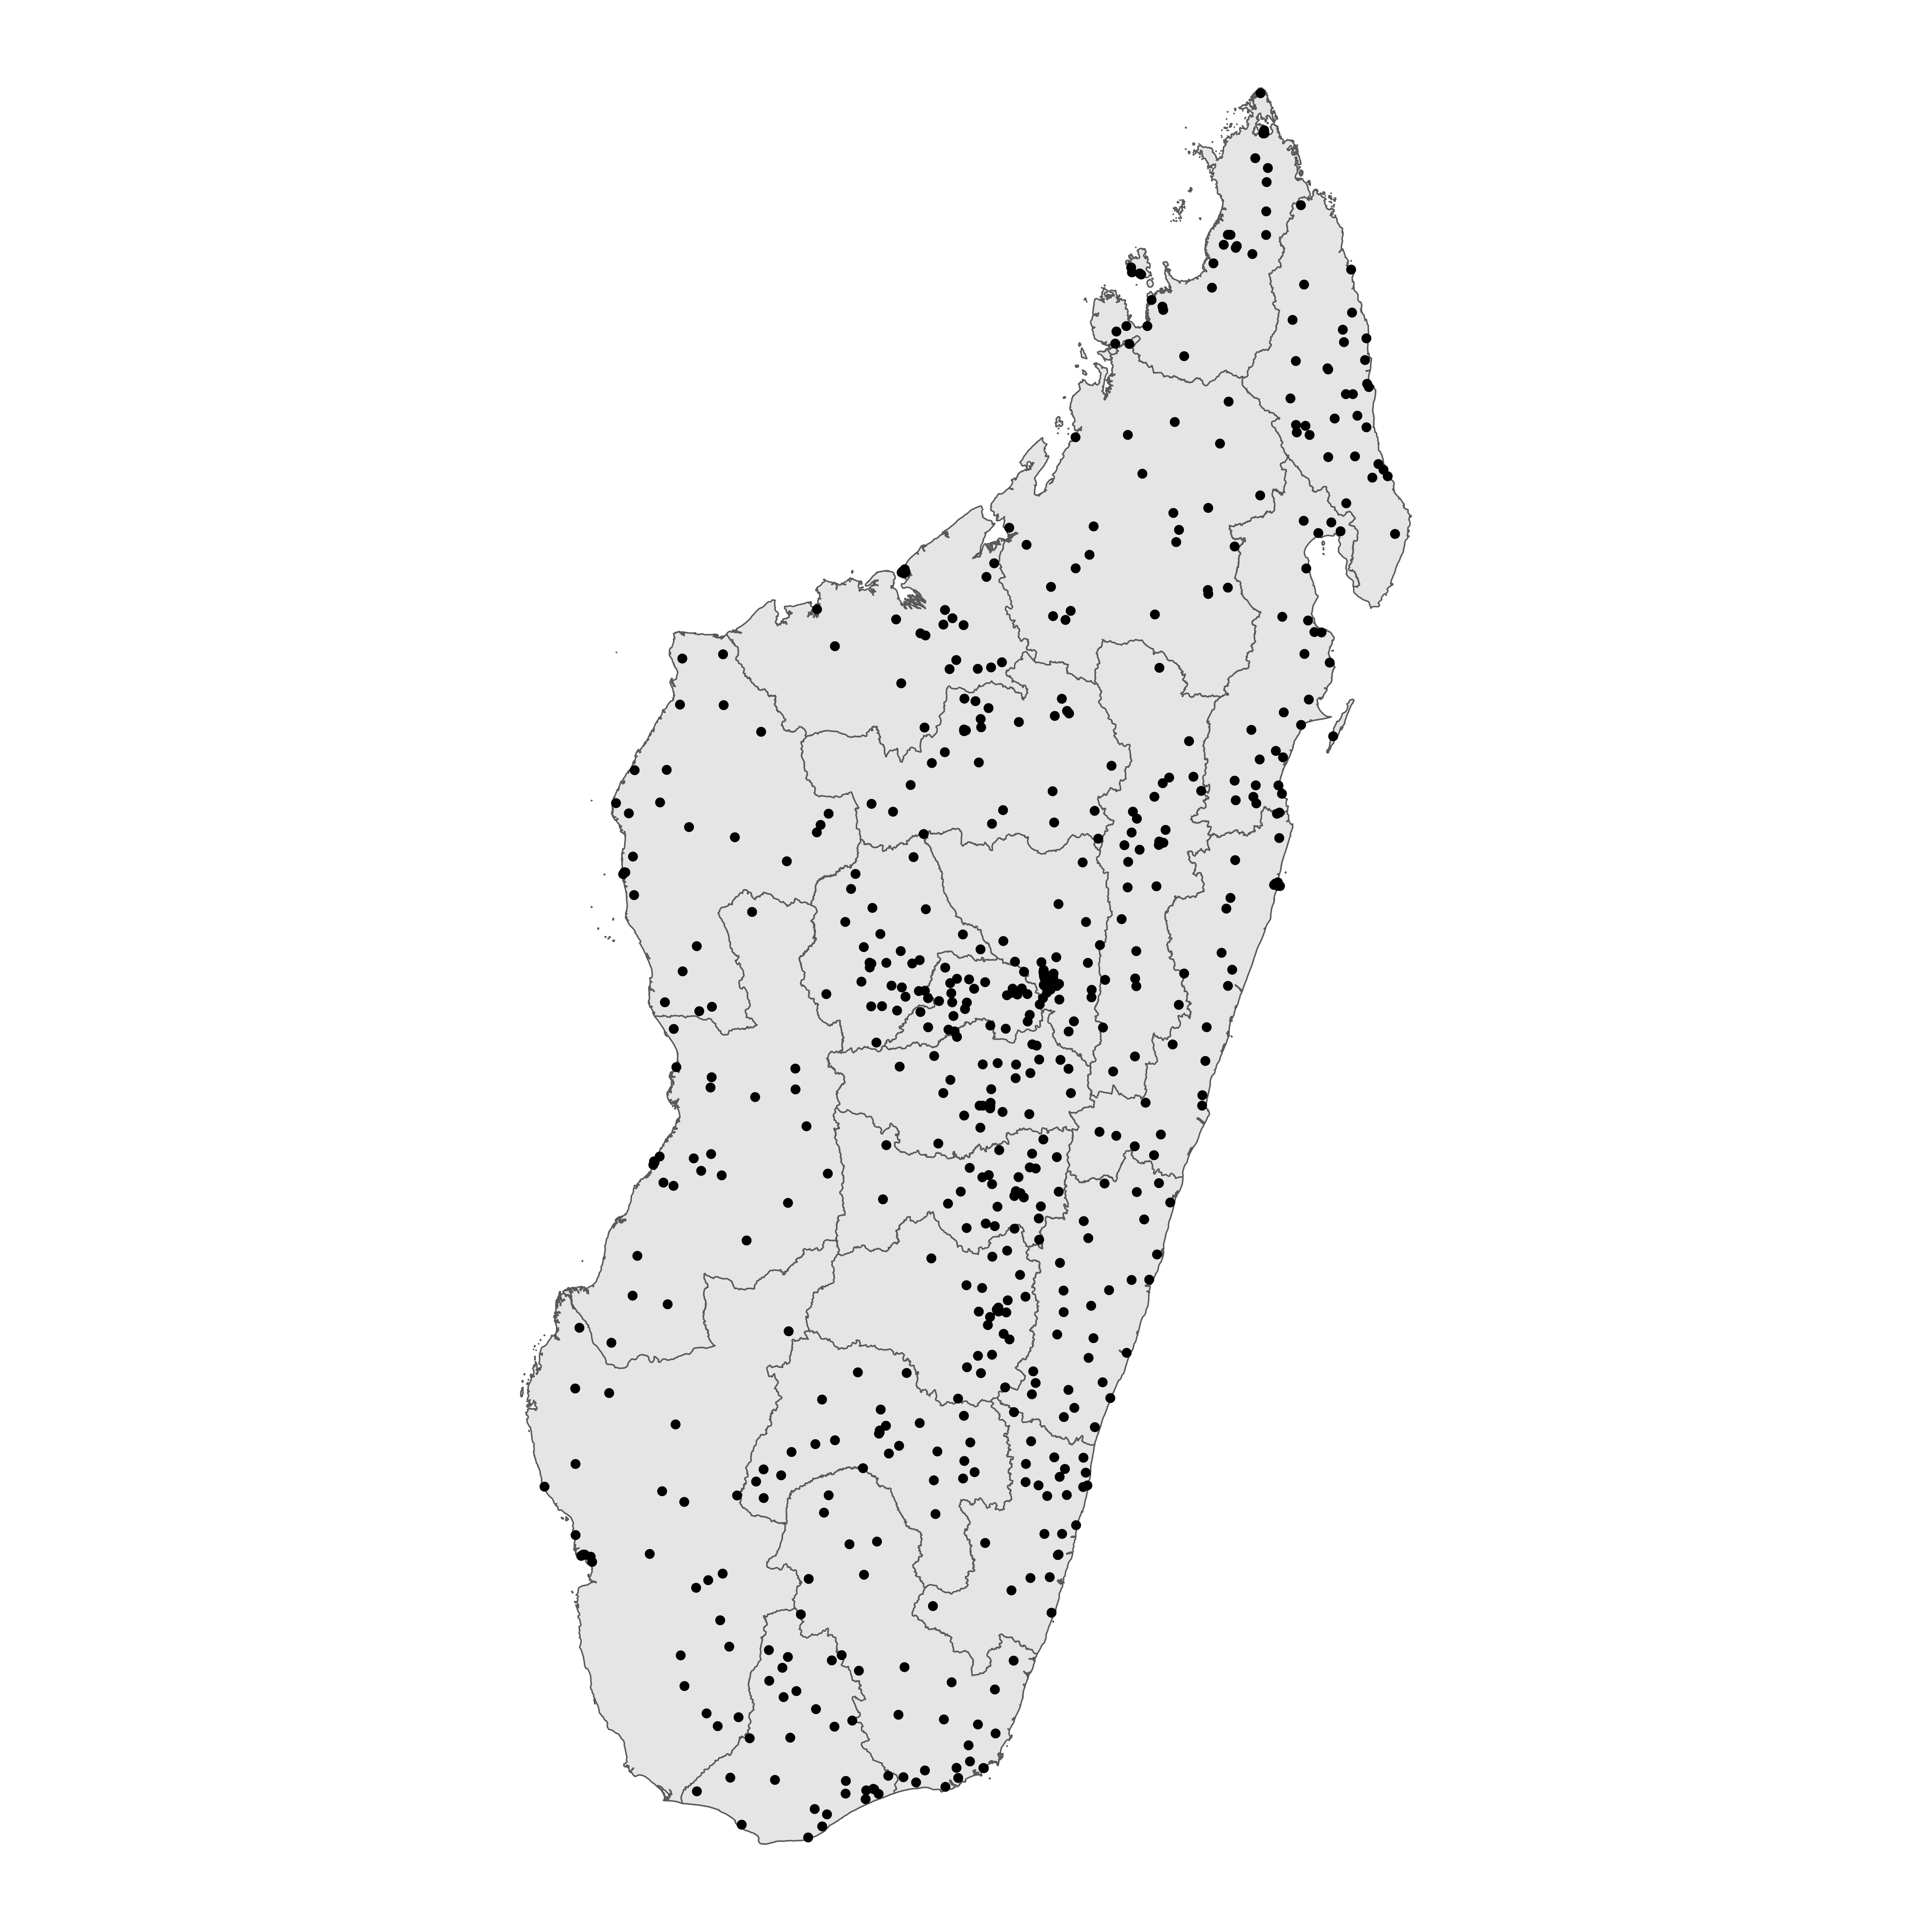
\includegraphics[width=0.8\textwidth, keepaspectratio]{figures/madagascar_clusterlocations.png}
	\caption{Childhood malnutrition in Madagascar: designated survey regions and cluster locations of the Madagascar 2021 Standard DHS.}
	\label{fig:madagascar_clusterloc}
\end{figure}

Correlates of childhood malnutrition are certainly not an understudied subject, publications that employ a variety of statistical approaches have been mentioned above. In the literature, two related trends can be identified. First, the shift to include remote sensed or satellite data to inform local environmental conditions and proxy economic shocks (see, for example, \textcite{graceConflictClimateFactors2022, vandermerweClimateChangeChild2022, seilerModellingChildrenAnthropometric2021}). Specifically, as research attempts to assess the effects of anthropogenic climate change on socio-economic and health outcomes, climatological variables present an important source of information. See \textcite{phalkeySystematicReviewCurrent2015} for a review of the research concerning malnutrition. Second, the shift to employing predictive approaches that stem from the machine learning community. This coincides with the need to include a larger number of explanatory variables facilitated by the availability of remotely sensed covariates. For example, \textcite{browneMultivariateRandomForest2021} suggest a multivariate random forest approach to predict wealth and malnutrition scores originating from DHS data jointly. \textcite{kimPrecisionMappingChild2021} map malnutrition indicators at high spatial resolution by first estimating cluster-level probabilities in a hierarchical regression and in a second step employing a semi-supervised regression approach to assign clusters to villages.

The component-wise boosting approach discussed herein is favourably suited to include a large number of (potentially uninformative) covariates to obtain effect selection for covariates of interest.


\subsubsection*{Madagascar 2021 Standard DHS}

The Madagascar 2021 Standard DHS was designed to provide estimates of population health indicators at the national level, the 22 administrative regions plus the capital, and for urban and rural populations. With the capital being urban only, this resulted in 45 strata. Based on the population census of 2018, a total of 657 clusters were drawn with probability proportional to population size, in each stratum independently. In each cluster, 34 households were drawn at random. This resulted in a sample size of 20'510 households, whereof 5'146 were urban and 15'364 rural \autocite{institutnationaldelastatistiqueinstatEnqueteDemographiqueSante2022}. \autoref{fig:madagascar_clusterloc} plots the boundaries of the survey regions and the locations of the survey clusters. 

\begin{figure}[!t]
	\centering
	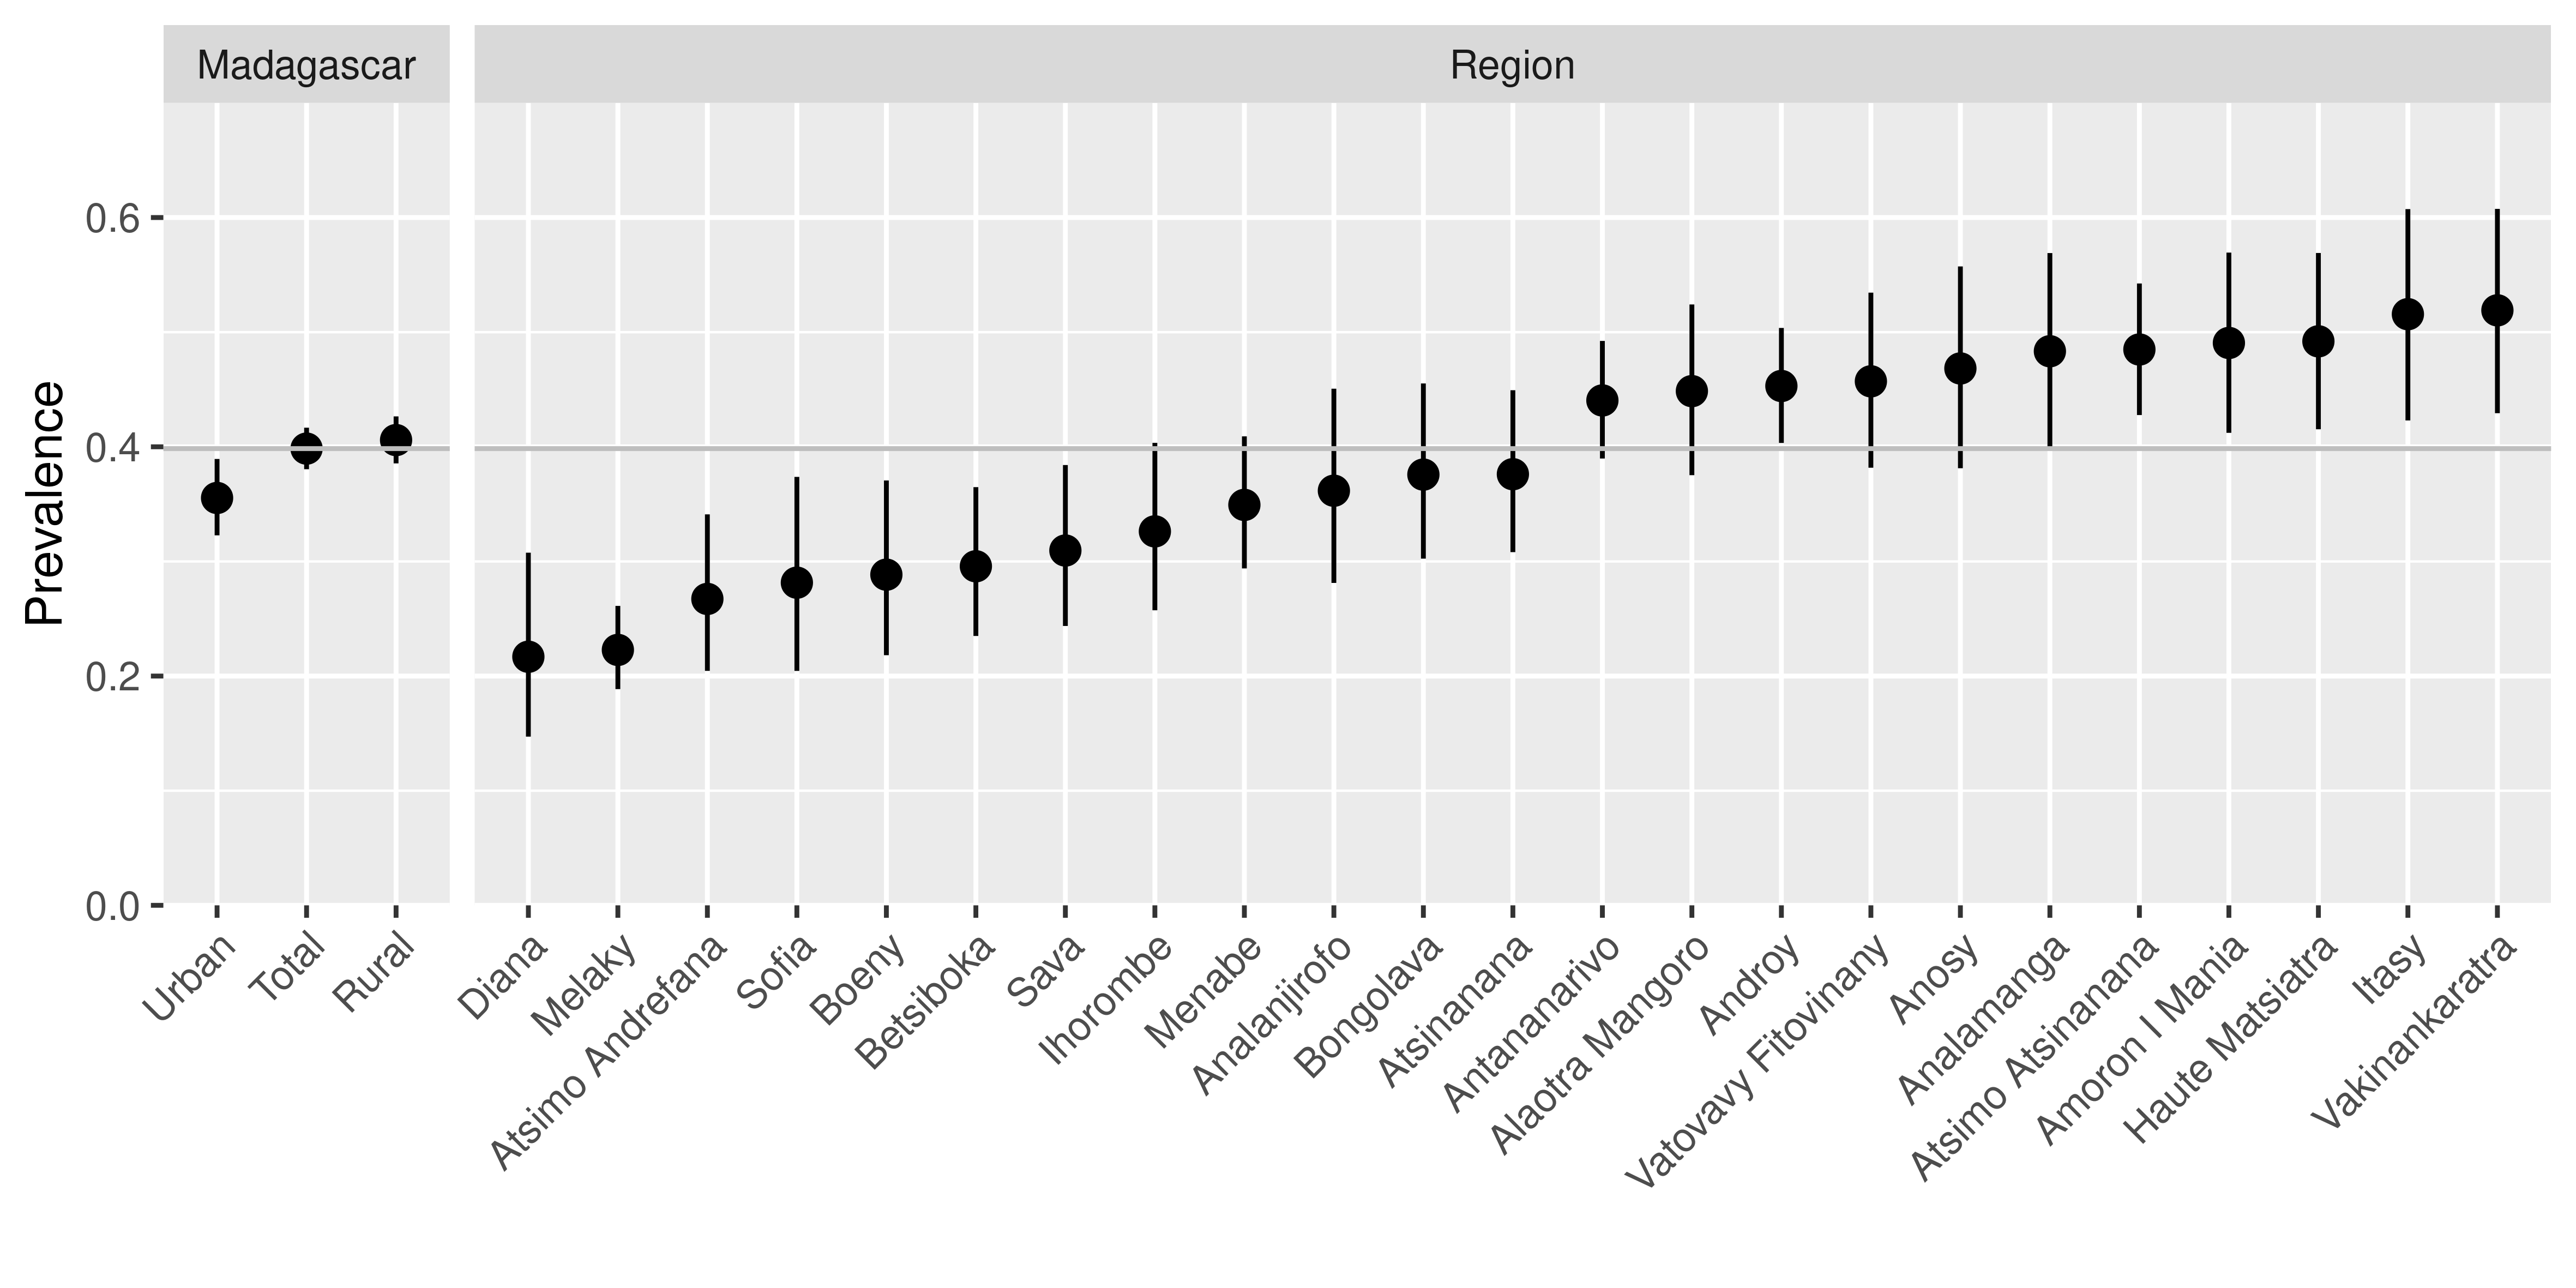
\includegraphics[width=0.9\textwidth, keepaspectratio]{figures/madagascar_designestimates.png}
	\caption{Childhood malnutrition in Madagascar: design-based estimates of prevalence of moderately or severely stunted children under 5 years. Error bars indicate 95\% confidence intervals. Data from the Madagascar 2021 Standard DHS.}
	\label{fig:madgascar_designestimates}
\end{figure}

The DHS surveys take anthropometric measurements from children under five years and provide the z-score of the height-for-age of each child. The analysis includes all children under five years and uses the binary indicator \textit{stunted} for all classified as moderately or severely stunted, that is, all children whose z-score is at least two standard deviations from the reference value. Further details on the compilation of the statistics can be found in \textcite{croftGuideDHSStatistics2020}. \autoref{fig:madgascar_designestimates} plots the design-based estimates of the regional and country-level prevalence with the corresponding confidence intervals. 


\subsubsection*{Explanatory variables}

As potential risk factors (or, conversely, protective factors), I include variables that previous research has considered in similar analyses. Specifically, the selection of explanatory variables is guided by the selection as discussed in \textcite{fenskeIdentifyingRiskFactors2011, fenskeUnderstandingChildStunting2013} and the references therein. Also, I further extend the selection of community-level factors with modelled covariates. Those are access to cities (i.e., access to markets and economic opportunities) and healthcare facilities. The covariates are provided at the grid-cell level and matched to the cluster location of an individual as the nearest grid-cell average. The selection is completed with a food security indicator provided by \textcite{fewsnetFEWSNETData2022} in the month preceding the survey. \autoref{tab:malnutritionpredictors} provides the description, type and corresponding source of all included covariates.

\begin{table}[!p]

    \begin{tabularx}{\textwidth}{lr}
        Covariate (Type)                    	& Source\\ \arrayrulecolor{black!30}\midrule
                                                & \\
    Individual                                  & \\ \arrayrulecolor{black!10}\midrule
        Age of the child in months (continuous) & Survey\\
        Duration of breastfeeding in months (continuous) & Survey\\
        Gender of the child (categorical: male, female) & Survey\\
        Indicator for twin children (categorical: no, yes) & Survey\\
        Position of the child in the birth order (categorical: 1, ..., 8+) & Survey\\
        Body mass index of the mother (continuous) & Survey\\
        Age of the mother in years (continuous) & Survey\\
        Years of education of the mother (continuous) & Survey\\
        Employment status of the mother (categorical: no, yes) & Survey\\
        Religion of the mother (categorical) & Survey\\
        Number of dead children (categorical: 0, 1, 2, 3+) & Survey\\
                                                & \\
    Household                                   & \\ \arrayrulecolor{black!10}\midrule      
        Number of household members (continuous) & Survey\\
        Source of drinking water (categorical: unimproved, improved, piped) & Survey\\
        Type of toilet facility (categorical: unimproved, improved) & Survey\\
        Wealth index (categorical: poorest, poorer, middle, richer, richest) & Survey\\
        Household has electricity supply (categorical: no, yes) & Survey\\
        Household has a radio (categorical: no, yes) & Survey\\
        Household has a television (categorical: no, yes) & Survey\\
        Household has a refrigerator (categorical: no, yes) & Survey\\
        Household has a bicycle (categorical: no, yes) & Survey\\
        Household has a motorcycle (categorical: no, yes) & Survey\\
        Household has a car (categorical: no, yes) & Survey\\
                                                & \\
    Community                                   & \\ \arrayrulecolor{black!10}\midrule
        Administrative region (categorical: 23 with neighbourhood structure)& Survey\\
        Place of residence (categorical: rural, urban) & Survey\\
        Walking time to healthcare facilities (continuous) & \textcite{weissGlobalMapsTravel2020}\\
        Travel-time to cities (continuous) & \textcite{weissGlobalMapTravel2018}\\
        Food security classification (categorical: 1-minimal, 2-stressed, 3-crisis) & \textcite{fewsnetFEWSNETData2022}\\
    \end{tabularx}

    \caption{Childhood malnutrition in Madagascar: individual, household and community-level predictors for chronic childhood malnutrition.}
    \label{tab:malnutritionpredictors}
    
\end{table}


\subsection{Modelling}

\subsubsection*{Model specification}

To estimate risk factors of stunting, I fit a logistic regression with the component-wise boosting described in \autoref{sec:methodology}. Let $y_i$ denote the classification status (0/1) of the child $i$ and model the outcome with a Bernoulli model
\begin{equation}
	y_i \sim \Bernoulli(\mu_i), \quad i = 1, \dots, N,
\end{equation}
where $i = 1, \dots, N$ are the children observed in the survey that are included in the analysis.\footnote{After the removal of data with missing characteristics a total of $N = 5722$ observations are included in the following analyses.} The relative probability of being stunted is estimated with a logistic additive predictor
\begin{align}\label{eq:madagascar_main}
	\begin{split}
	\logit (\mu_i) &= \eta_i\\
	&= \beta_0 + \sum_{j = 1}^{p} \beta_j x_{ji} + \sum_{k = 1}^{q} f_{\mathtt{smooth}} (x_{ki}) + f_{\mathtt{spatial}} (x_{\text{region[i]}}), \quad i = 1, \dots, N.
	\end{split}
\end{align}
The loss function is specified as the negative binomial log-likelihood. Categorical covariates are included as linear effects, and treatment coded. Smooth effects for continuous covariates are cubic P-splines with second-order differences and 20 inner knots. To allow for effect selection between linear and non-linear effects for continuous covariates, the smooth effects are included in the parametric and centred decomposition described before. Lastly, to account for the cumulative effect of unidentified covariates on a regional level, I include a spatial effect for the survey regions by adding a Markov random field effect induced by the first-order neighbourhood structure.\footnote{As discussed in \autoref{sec:demographic-and-health-surveys}, the individual survey responses are assigned a sampling weight. In the literature, the use of survey weights in regression is debated. See for instance \textcite{winshipSamplingWeightsRegression1994, gelmanStrugglesSurveyWeighting2007}. The parameter estimates estimated by boosting are regularised and therefore likely not consistent concerning the true population value. Furthermore, it is not clear how to correct the weights when subsampling the survey data, since the sampling weights are post-stratified to correct for non-response. Though it is possible to include observation weights in this approach -- all learners can be estimated by penalised weighted least squares -- I omit those for the following analyses.}

In the following, I also briefly consider several alternative specifications of the additive predictor. First, as a sensible baseline, I consider a simple linear model. Second, to test a successive increase in implemented model complexity, an augmented linear model where all first-order interactions are added is considered. Third, I consider \autoref{eq:madagascar_main} where each covariate additionally interacts with either (1) the gender of the child or (2) the urbanicity status. As a non-parametric approach, I also test boosted regression trees with a maximum depth of four, and with all other parameters left at their default values. The latter model should provide insights of whether higher-order interactions are present in the data.


\subsubsection*{Model evaluation and selection}

\begin{figure}[t!]
	\centering
	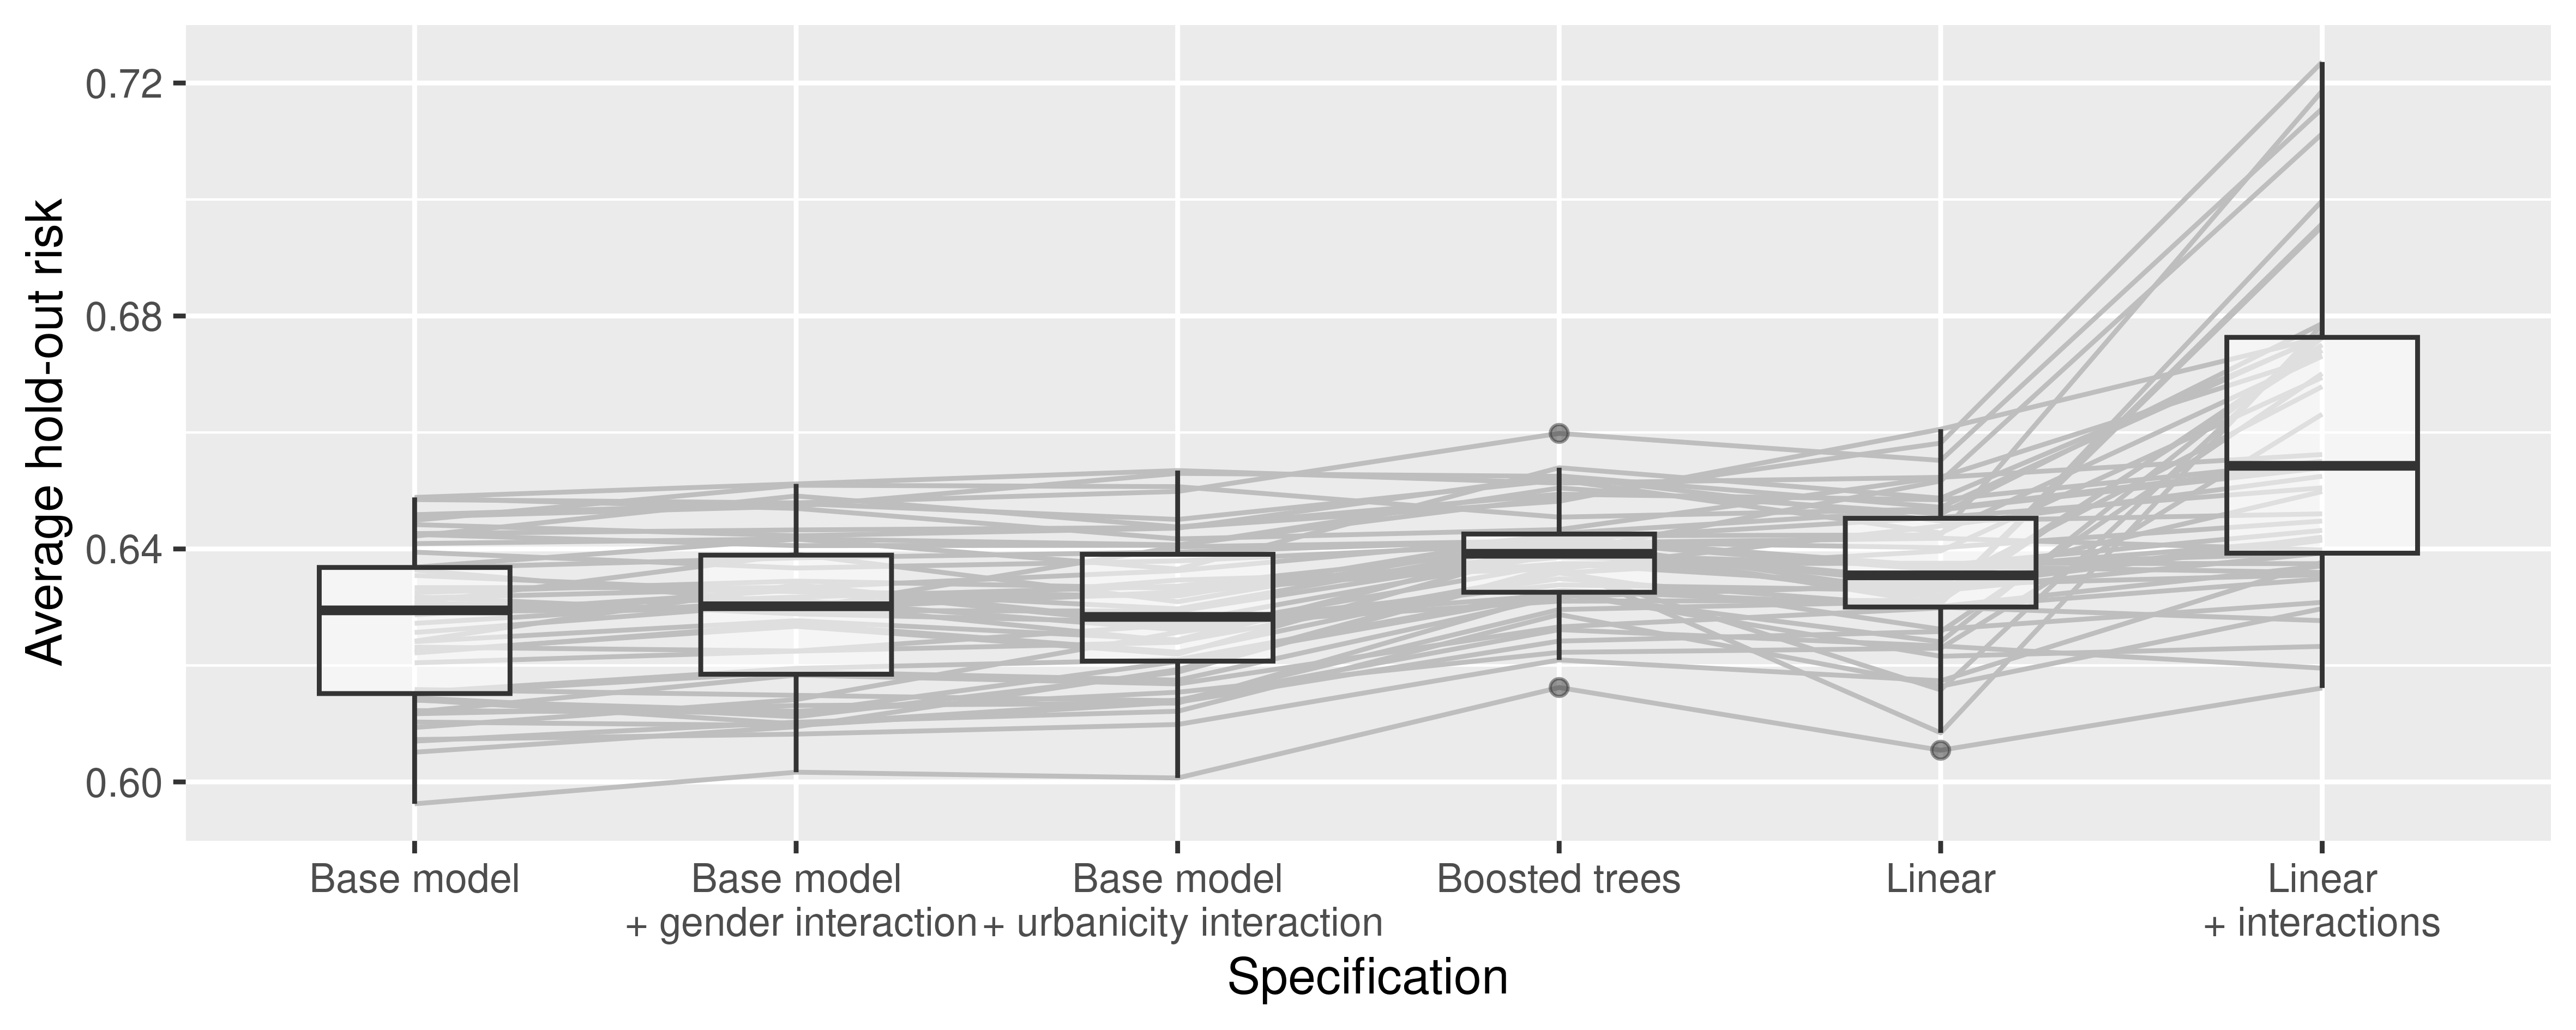
\includegraphics[width=0.9\textwidth, keepaspectratio]{figures/madagascar_modelselection.png}
	\caption{Childhood malnutrition in Madagascar: comparison of different model specifications. Lower is better. Grey lines indicate the average test-set error (predictive risk). Empirical distributions over 50 replications.}
	\label{fig:madagascar_modelselection}	
\end{figure}

As discussed in \autoref{sec:methodology}, early stopping is applied to the algorithm to prevent over-fitting and obtain a model that generalises well on unseen data. For the following results, given the larger number of samples, I use the 2 or 3-way holdout method to fit the model on a training set, select the number of boosting iterations by where the minimum predictive risk is attained on the validation set, and use test-set performance to select between models. For the model evaluation part, I use approximately 70/20/10 splits and for the final results in the following part 80/20. All folds are stratified by the survey strata to acknowledge the survey design. Throughout this section, I fix the hyper-parameter $\nu = 0.1$.

\autoref{fig:madagascar_modelselection} plots the average test-set risk of 50 replications. Seemingly, compared to the base model, the additional flexibility of the augmented models does not translate into improved generalisation performance. The linear model does not yield the same performance as the base specification, underscoring the necessity to capture non-linearities in associated risk factors. That coincides with previous literature \autocite{fenskeIdentifyingRiskFactors2011, kandalaGeoadditiveModelsChildhood2009}. But the differences are also not markedly different. Clearly, the linear model with all interactions seems unstable, and the hold-out risk varies strongly. Interestingly, boosting trees do not yield the same performance, but are more stable (lower variance) across replications. Altogether this provides evidence against higher-order interactions in the data. For the remainder of this analysis, I turn to the base specification as provided in \autoref{eq:madagascar_main}.


\subsection{Results}

For the following results, I show for each covariate the estimated partial effect from 50 replications of the train-validation split. This subsampling approach allows for an idea of the stability of the estimated parameters \autocite{meinshausenStabilitySelectionStability2010}. The inclusion frequency over the replications is provided in the supplementary material.

\begin{figure}[t!]
	\centering
	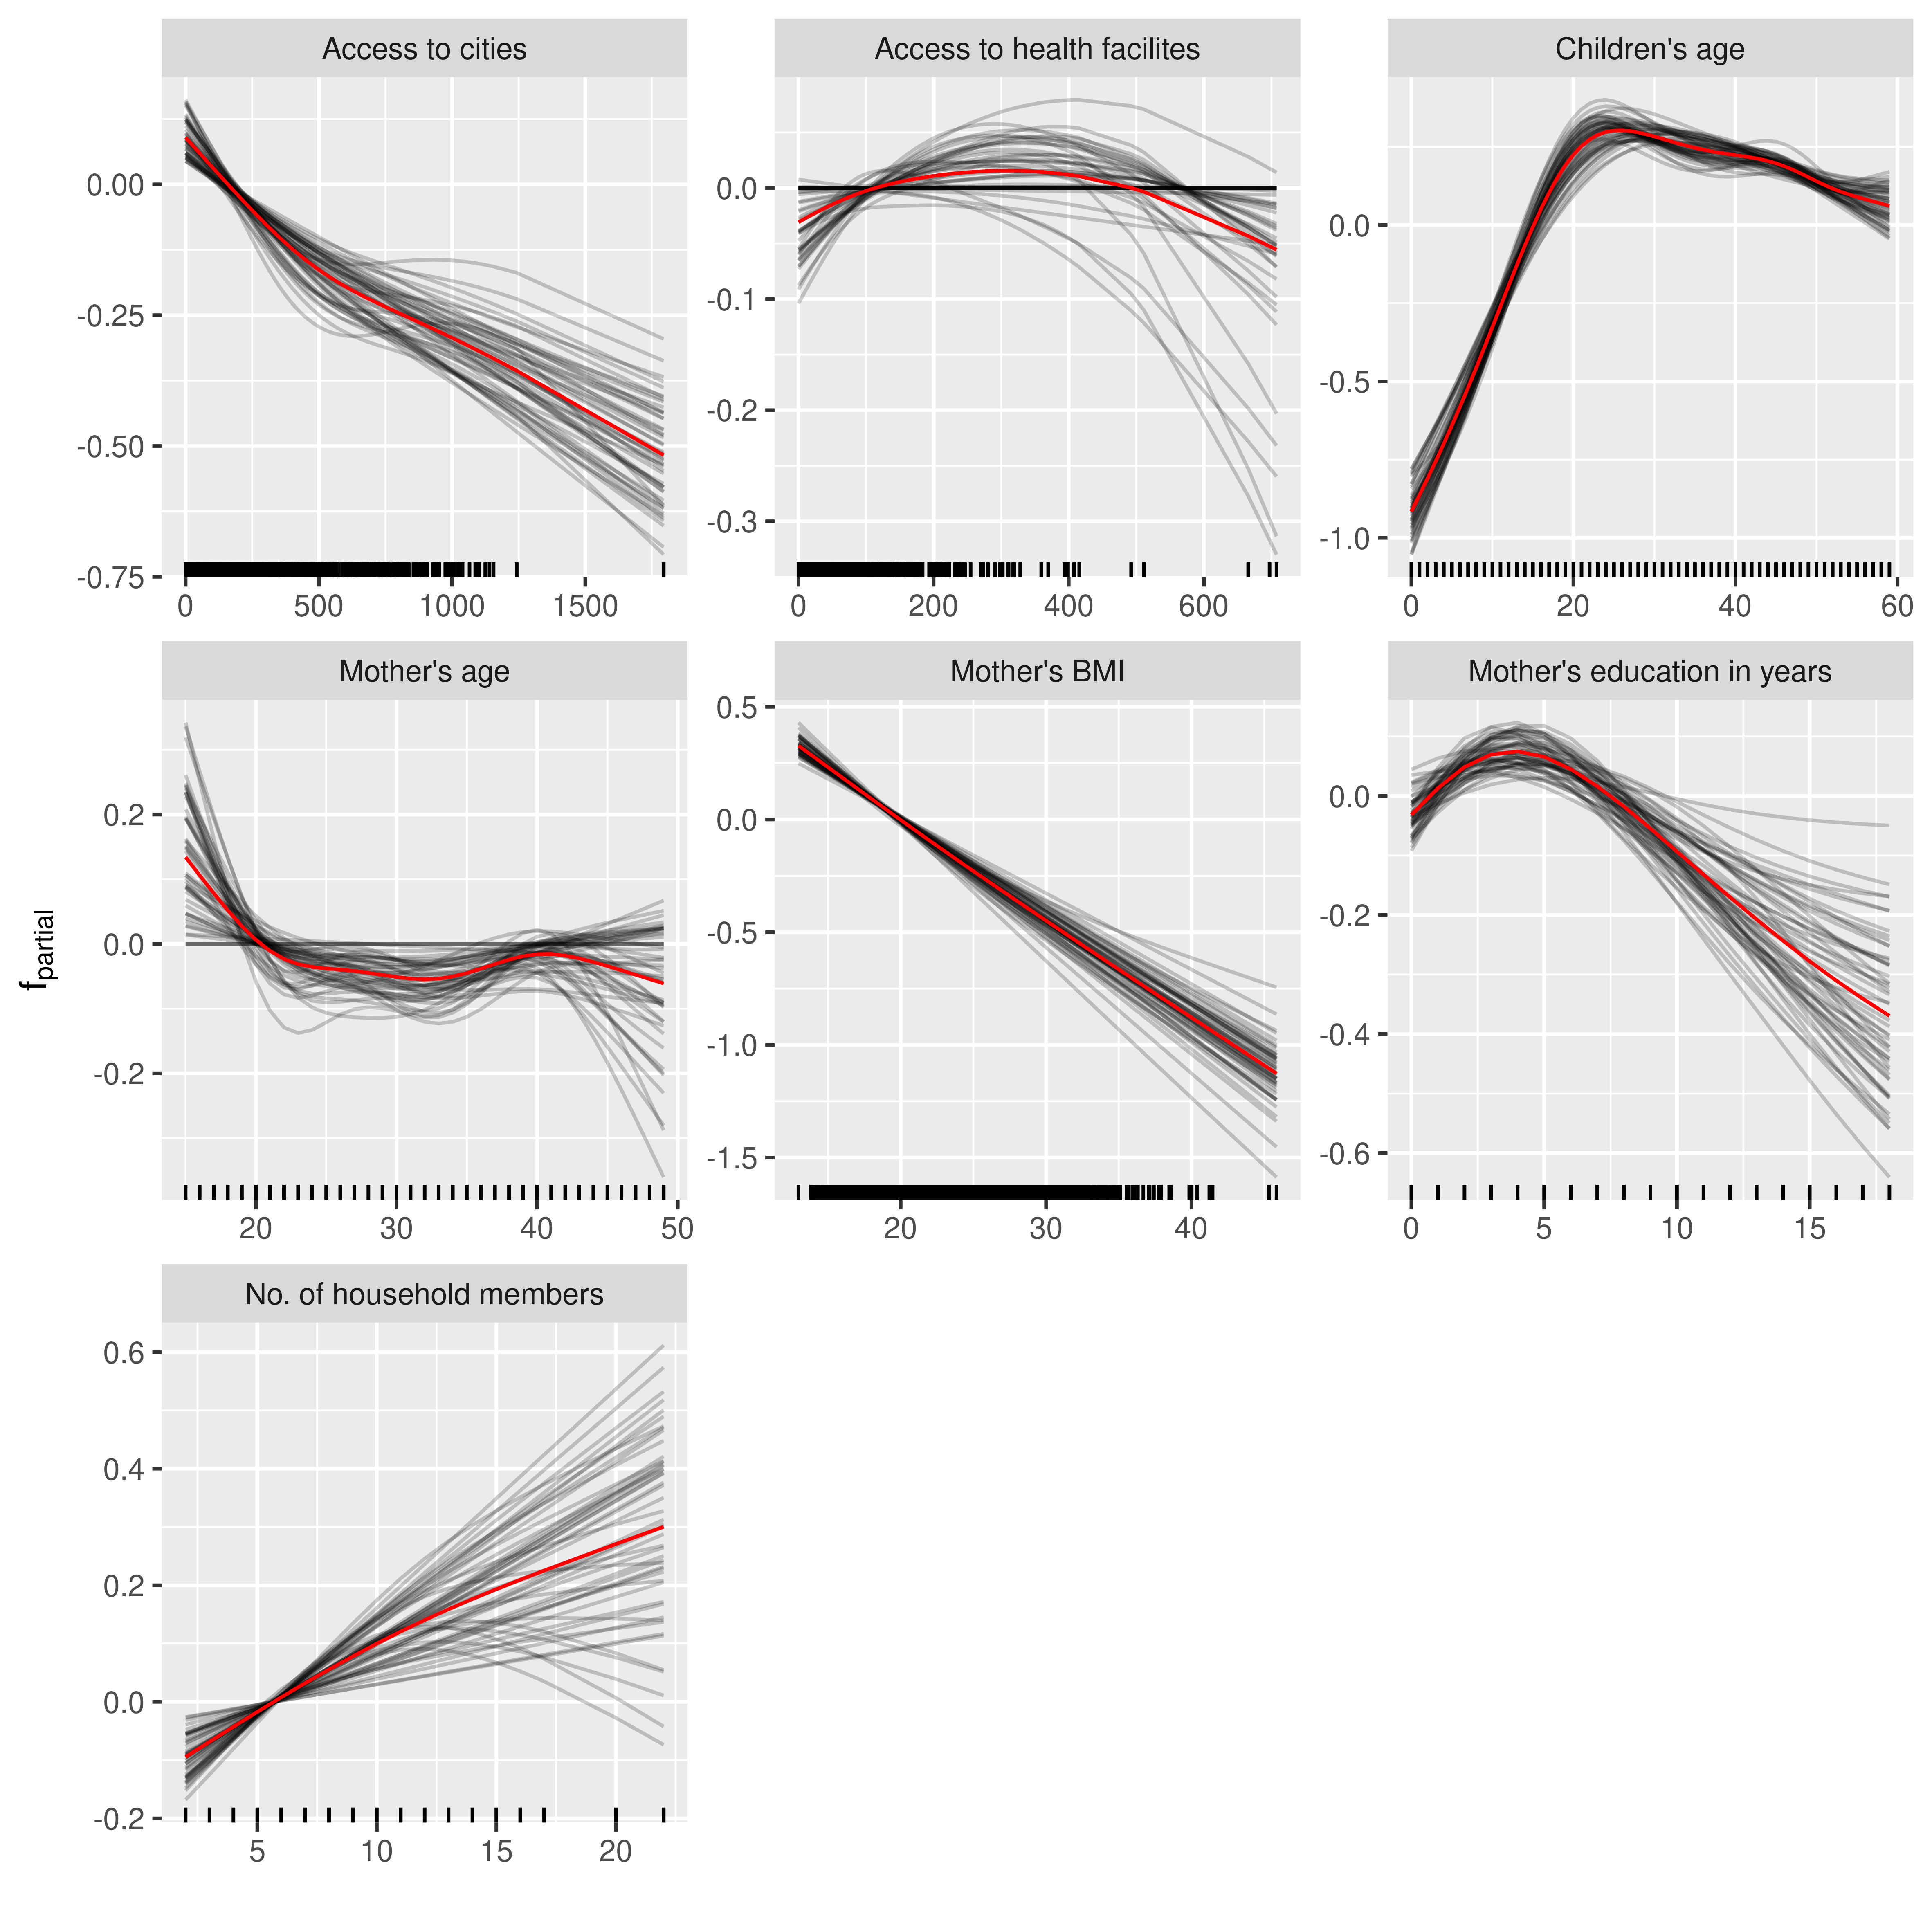
\includegraphics[width=\textwidth, keepaspectratio]{figures/madagascar_smootheffects.png}
	\caption{Childhood malnutrition in Madagascar: partial effects of the continuous covariates. The red line indicates the pointwise average and the grey lines indicate the estimated effects from 50 replications.}
	\label{fig:madagascar_smootheffects}
\end{figure}

Beginning with the continuous covariates we find a negative partial effect of access to cities, indicating that higher distance to cities is associated with an increased risk of stunting (\autoref{fig:madagascar_smootheffects}). Access to healthcare is inversely U-shaped but often estimated to be zero. The linear effect was included only in 36\% of the replications and the non-linear deviation in 68\%. The effect estimates of the children's age are very stable, with very young ages having a protective factor, the partial effect increasing until the age of 20 months. The mother's age is inversely U-shaped with very young ages being a risk factor. For higher ages ($>$40 years) the estimation of the effect is much more variable. The partial effect of stunting is decreasing with the mother's BMI and increases with the number of household members, both estimated (mostly) to be linear, although the latter with much more variability in the slope. The mother's education shows an inversely U-shaped partial effect, with lower values accumulated around zero and a protective risk factor for a higher number of years in education. 

\begin{figure}[!t]
	\centering
	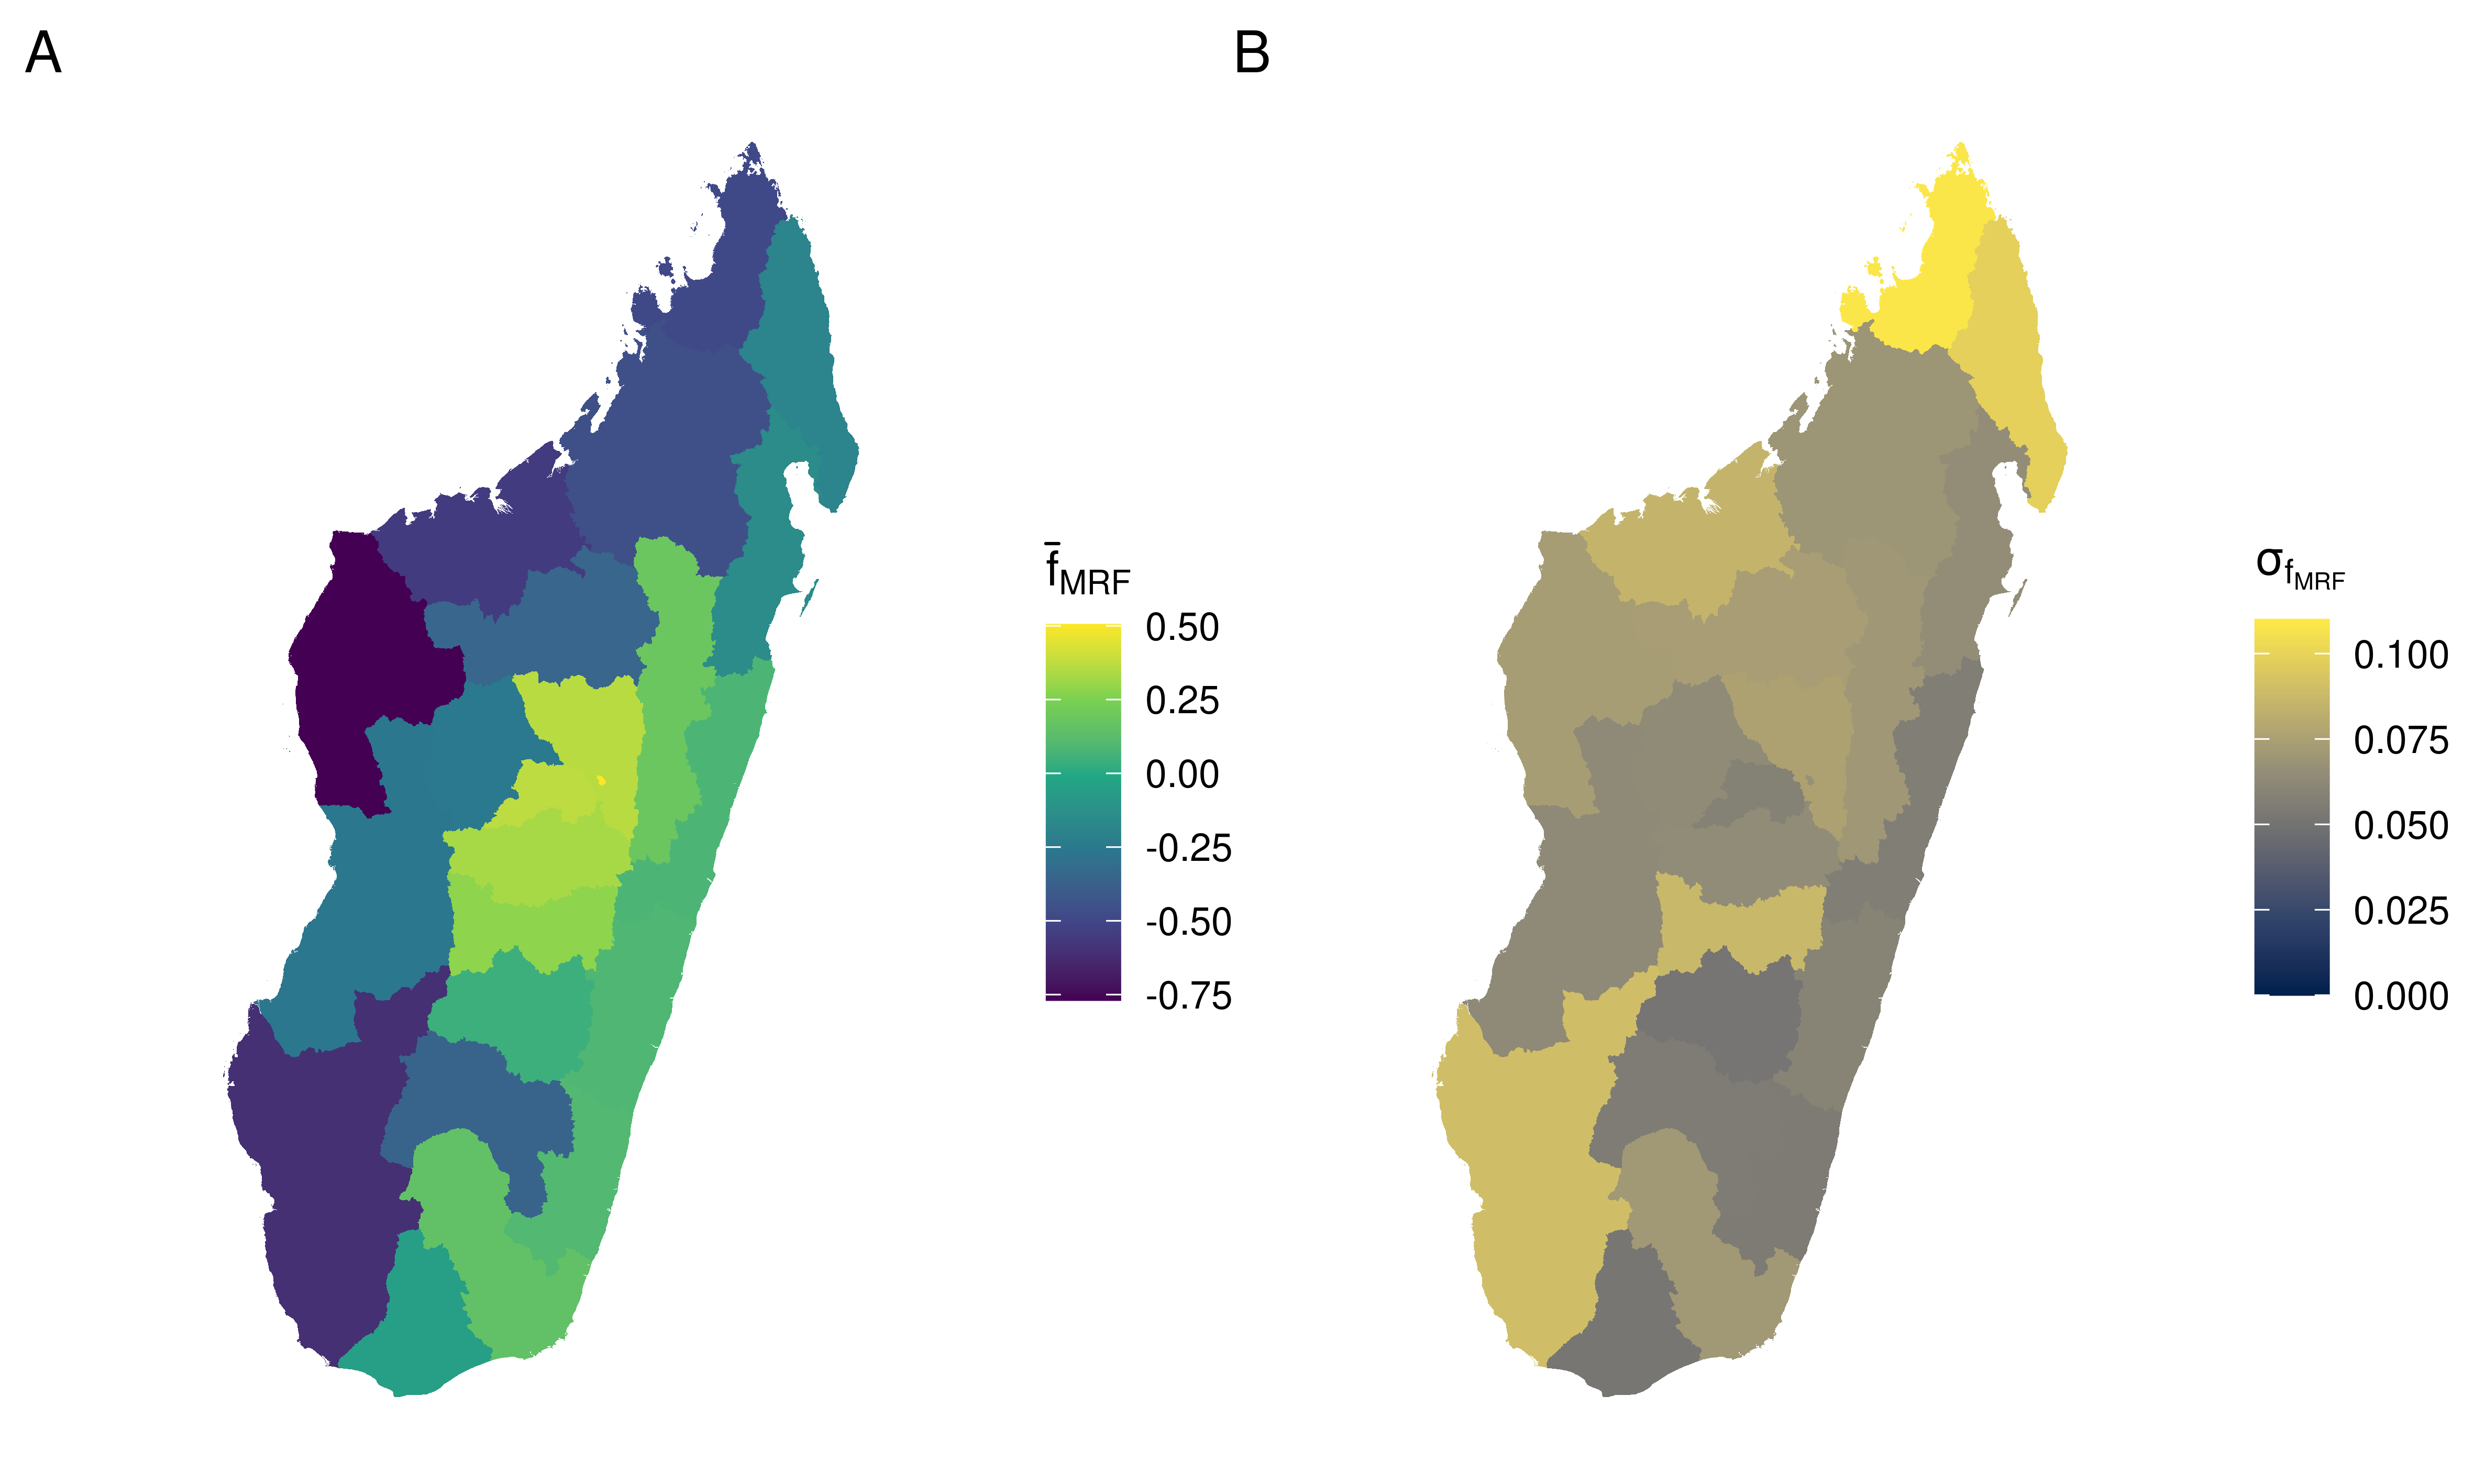
\includegraphics[width=0.9\textwidth, keepaspectratio]{figures/madagascar_spatialeffects.png}
	\caption{Childhood malnutrition in Madagascar: estimated discrete spatial effect. Panel A: mean effect over 50 replications. Panel B: standard deviation of the estimated effects.}
	\label{fig:madagascar_spatialeffects}
\end{figure}

\autoref{fig:madagascar_spatialeffects} shows the mean and standard deviation of the estimated discrete spatial effect. Eastern regions of the island show an excess risk towards stunting. Generally, the south (-east) is considered the most afflicted area in terms of food security \autocite{fewsnetFEWSNETData2022}.

\begin{figure}[!p]
	\centering
	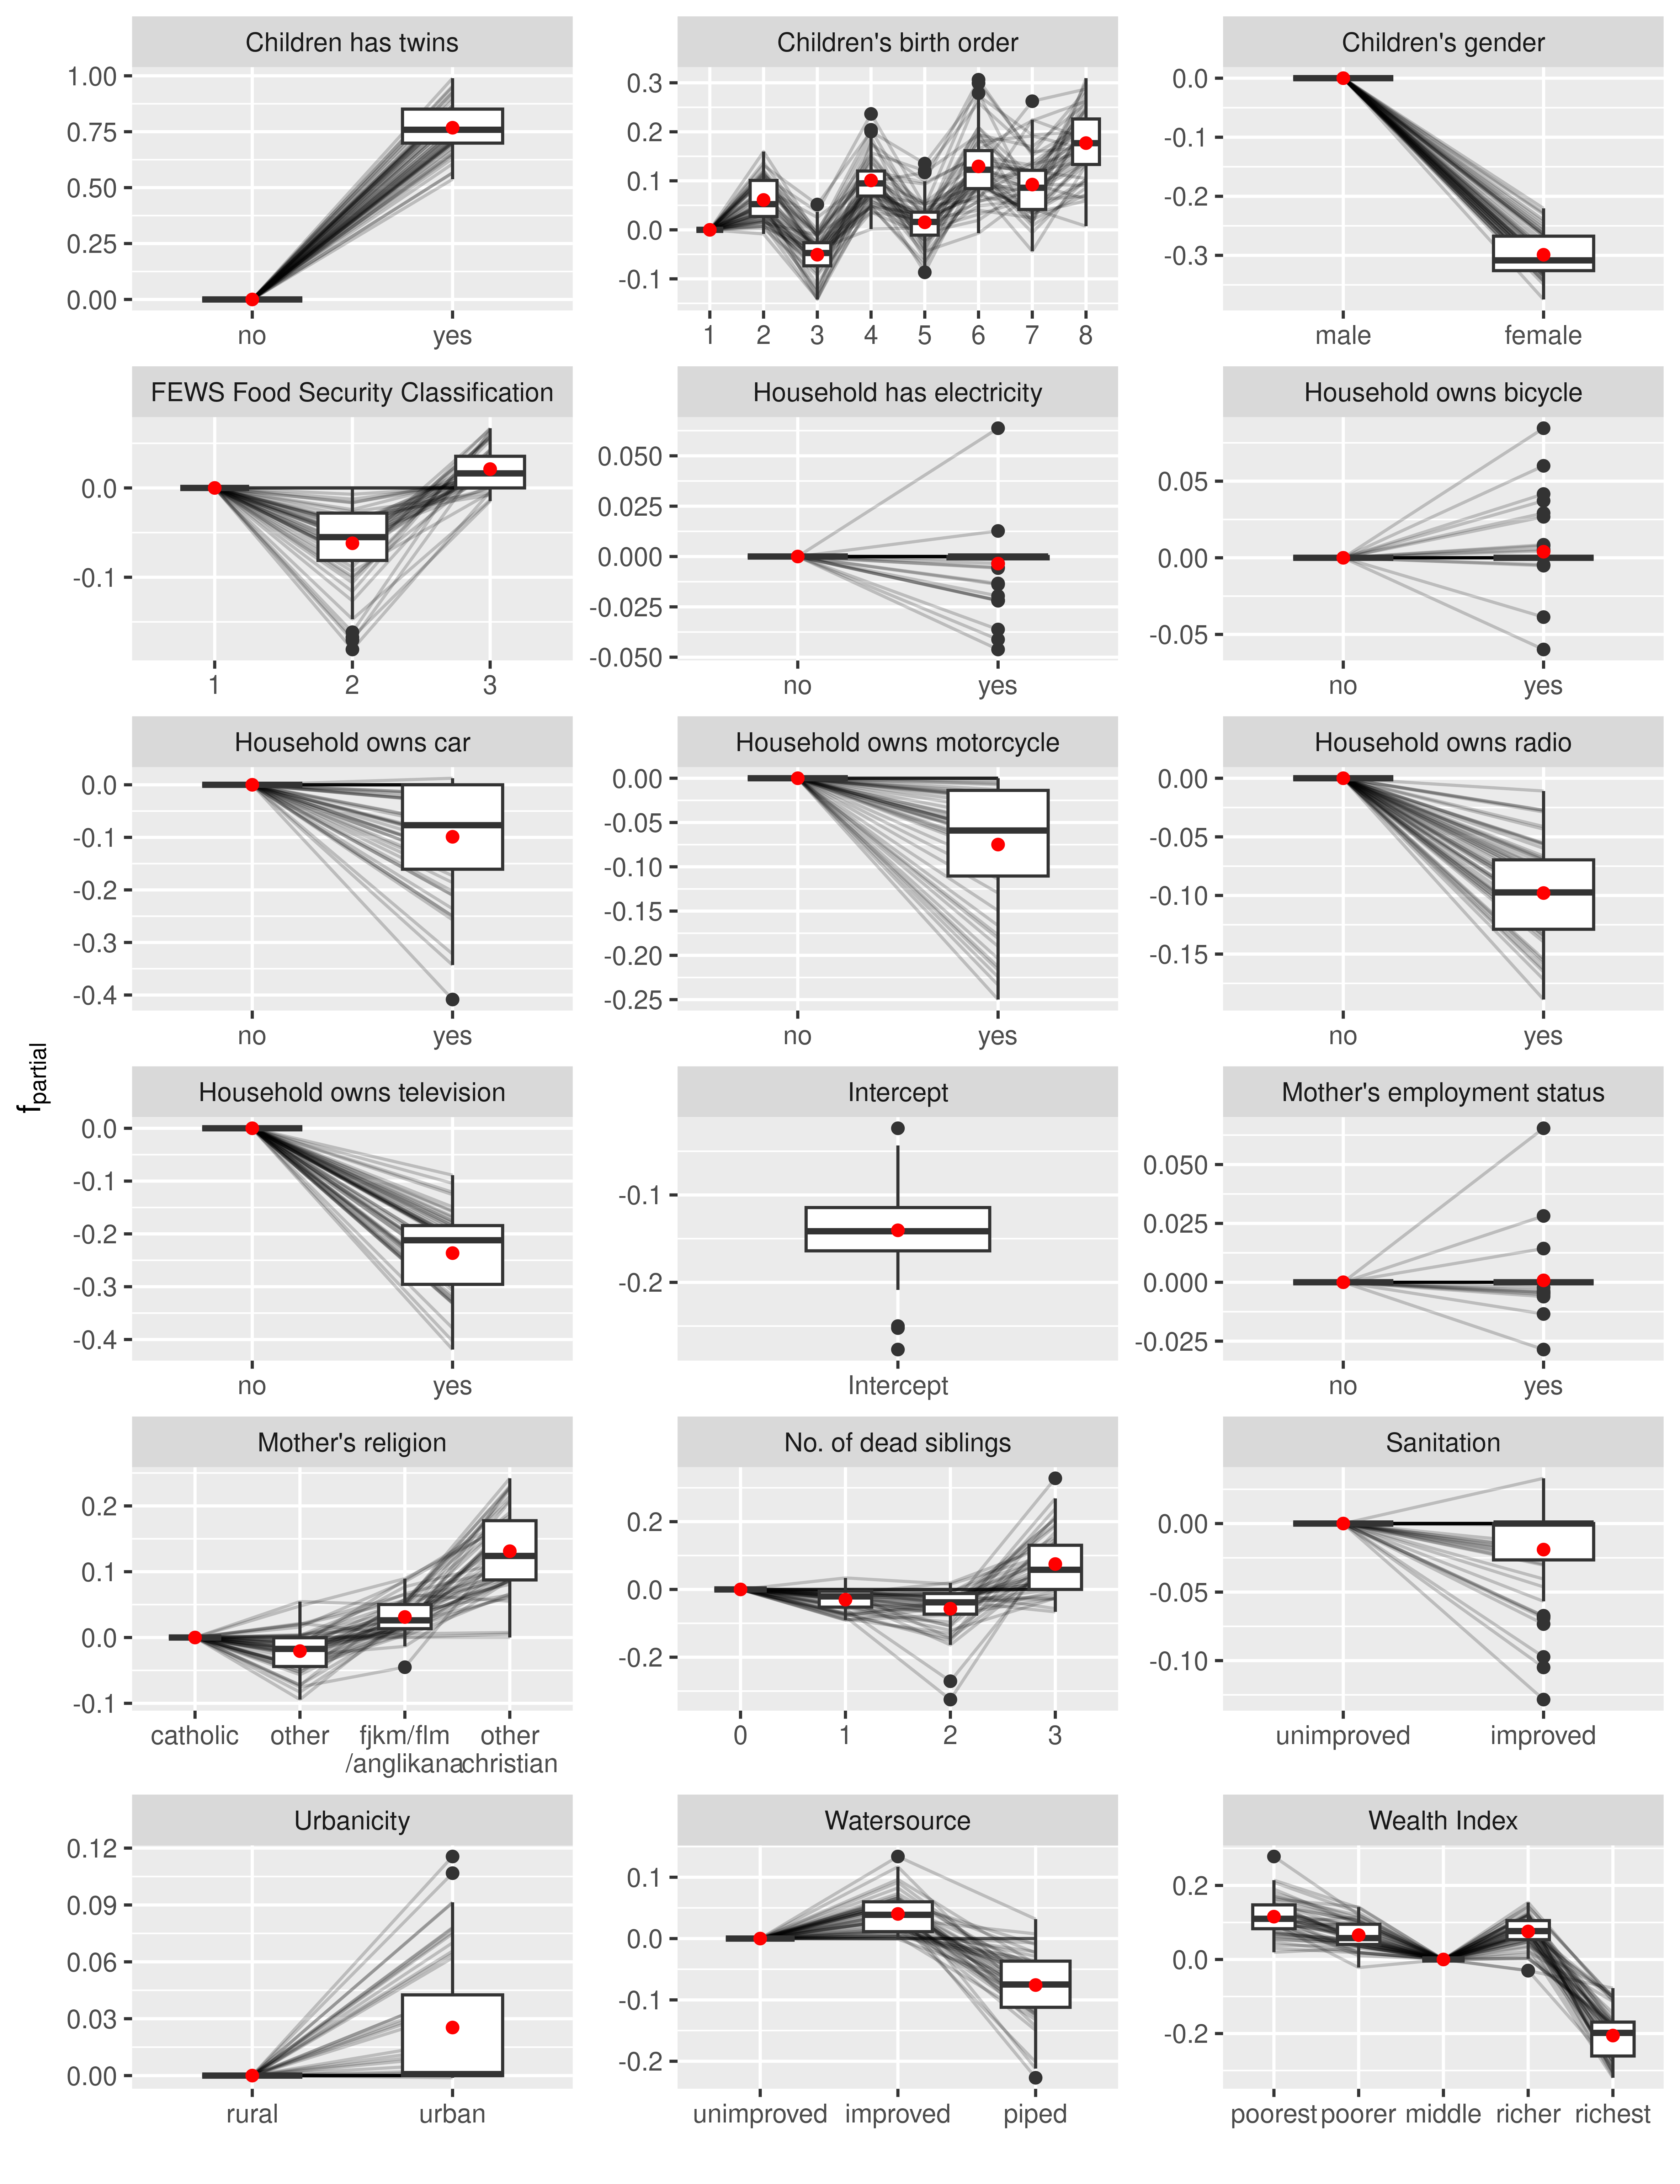
\includegraphics[width=\textwidth, keepaspectratio]{figures/madagascar_categoricaleffects.png}
	\caption{Childhood malnutrition in Madagascar: estimated categorical coefficients. Grey lines indicate the 50 replications, and the red point indicates the pointwise average of the estimated coefficients.}
	\label{fig:madagascar_categoricaleffects}
\end{figure}

Lastly, a review of selected categorical effects. For most indicators associated with wealth, those are a protective factor (car, radio, television, etc.). Similarly, being in the richest quantile of the population (DHS wealth category). The children's gender (female vs. male) has a negative partial effect, i.e., decreased risk of being stunted, which is in line with the observation that the prevalence of stunting is higher among boys than girls \autocite[][p. 10]{unicefImprovingChildNutrition2013}. Higher birth order is associated with a higher log-odds ratio of being stunted. Note, the effect of the birth order can not be interpreted as a within-household effect because the anthropometric measures in the DHS sample are age-censored.\footnote{See \cite{spearsEndogenousInclusionDemographic2022} for further discussion on this topic.}

In the supplementary material, I present the empirical distributions of the 'importance' of each component of the additive predictor. The highest contribution to the reduced risk is the spatial effect indicating the need for an improved understanding of regional-level risk factors of chronic childhood malnutrition. Other variables that contributed the most to the reduction were the children's age, the mother's BMI, access to cities, and the children's gender. 

The component-wise boosting approach allows for important insights into the model, and, in this setting, allows for inference about the functional form of an effect. For instance, the child's age as a risk factor is estimated non-linear across the range. Furthermore, stability selection can be employed to obtain type-1 error controls for variable selection \autocite{meinshausenStabilitySelectionStability2010, shahVariableSelectionError2013}. Thus, the preliminary results for the interested reader are presented in the enclosed code repository.



\section{Geographic malaria risk in Mali}\label{sec:geographic-malaria-risk-in-mali}

In the second case study, we turn to cluster-level estimates of malaria prevalence.\footnote{Note, the term \textit{prevalence} refers to the empirical proportion of the population experiencing the condition while the term \textit{risk} refers to the analogue of the hypothetical infinite population \autocite{fuglstadTwoCulturesPrevalence2022}.} Specifically, the objective of this case study is to identify environmental correlates of local malaria prevalence for children below the age of five and predict the estimated risk at a high spatial resolution. A similar study was presented in \textcite{giardinaBayesianVariableSelection2016}, where the authors propose a Bayesian variable selection based on Dirichlet priors and a non-stationary Gaussian spatial process to model residual spatial variation at the transition of ecological zones. In this case study, I employ the component-wise boosting approach to obtain effect selection.  


\subsection{Introduction}

Malaria is an infectious disease for humans, caused by the \textit{Plasmodium spp.} when transmitted by a bite of an infected female \textit{Anopheles} mosquito. Most common are the \textit{Plasmodium falciparum} and \textit{Plasmodium vivax} species, the two variants account for the majority of cases \autocite{phillipsMalaria2017}. Untreated, severe malaria can be fatal, with the highest burden among young children below the age of five. Cases and deaths have declined since 2000, albeit slowly, with a recent up-tick likely due to the COVID-19 pandemic. For 2020, the latest data at the time of writing, the WHO estimates 241 million cases and 627'000 deaths \autocite{worldhealthorganizationWorldMalariaReport2021}. Globally, high-transmission countries in sub-Saharan Africa accounted for a large share of malaria cases in the 85 countries where malaria is endemic: 29 countries accounted for 96\% of all the cases and deaths. Of all child deaths below the age of five, malaria is estimated to account for 7.8\%. The country in this analysis, Mali, whilst only with a population of about 22 million, is estimated to represent 3\% of the \textit{global} caseload. Undoubtedly, the health and economic burden on households and countries is substantive and long-lasting. In country-level studies, micro-evidence from early eradication campaigns of malaria suggests that exposure early in life does shape (long-term) economic outcomes \autocite{bleakleyMalariaEradicationAmericas2010, cutlerEarlyLifeMalariaExposure2010, lucasMalariaEradicationEducational2010, hongMalariaEconomicProductivity2011}. 

Household surveys routinely collect information on malaria-related indicators, such as the ownership and use of insecticide-treated mosquito nets. The Malaria Indicator Surveys (MIS) from the DHS program are a format analogous to the standard DHS surveys but tailored to collect malaria-related information. In selected countries, additional samples are taken from populations at risk to establish the infection of the individual. In particular, those surveys are conducted during the high malaria transmission season of the respective country. The following study is based on the Mali 2021 Malaria Indicator Survey (MIS) where children between 6-59 months were tested for malaria with Rapid Diagnostic Tests (RDTs).\footnote{Some household surveys use Polymerase Chain Reactions (PCR) tests identify malaria infection rather than Rapid Diagnostic Tests (RDTs). PCR tests generally have a higher sensitivity than RDT tests at the expense of higher costs. Therefore, prevalence estimates from both testing methods should not be compared directly. \textcite{floreyMeasuresMalariaParasitemia2014} assess differences in estimates in DHS surveys where both test methods were used, concluding that RDTs may be sufficient to identify populations with higher risk but should not be used to assess the effectiveness of health interventions.} 

\begin{figure}[!t]	
	\centering
	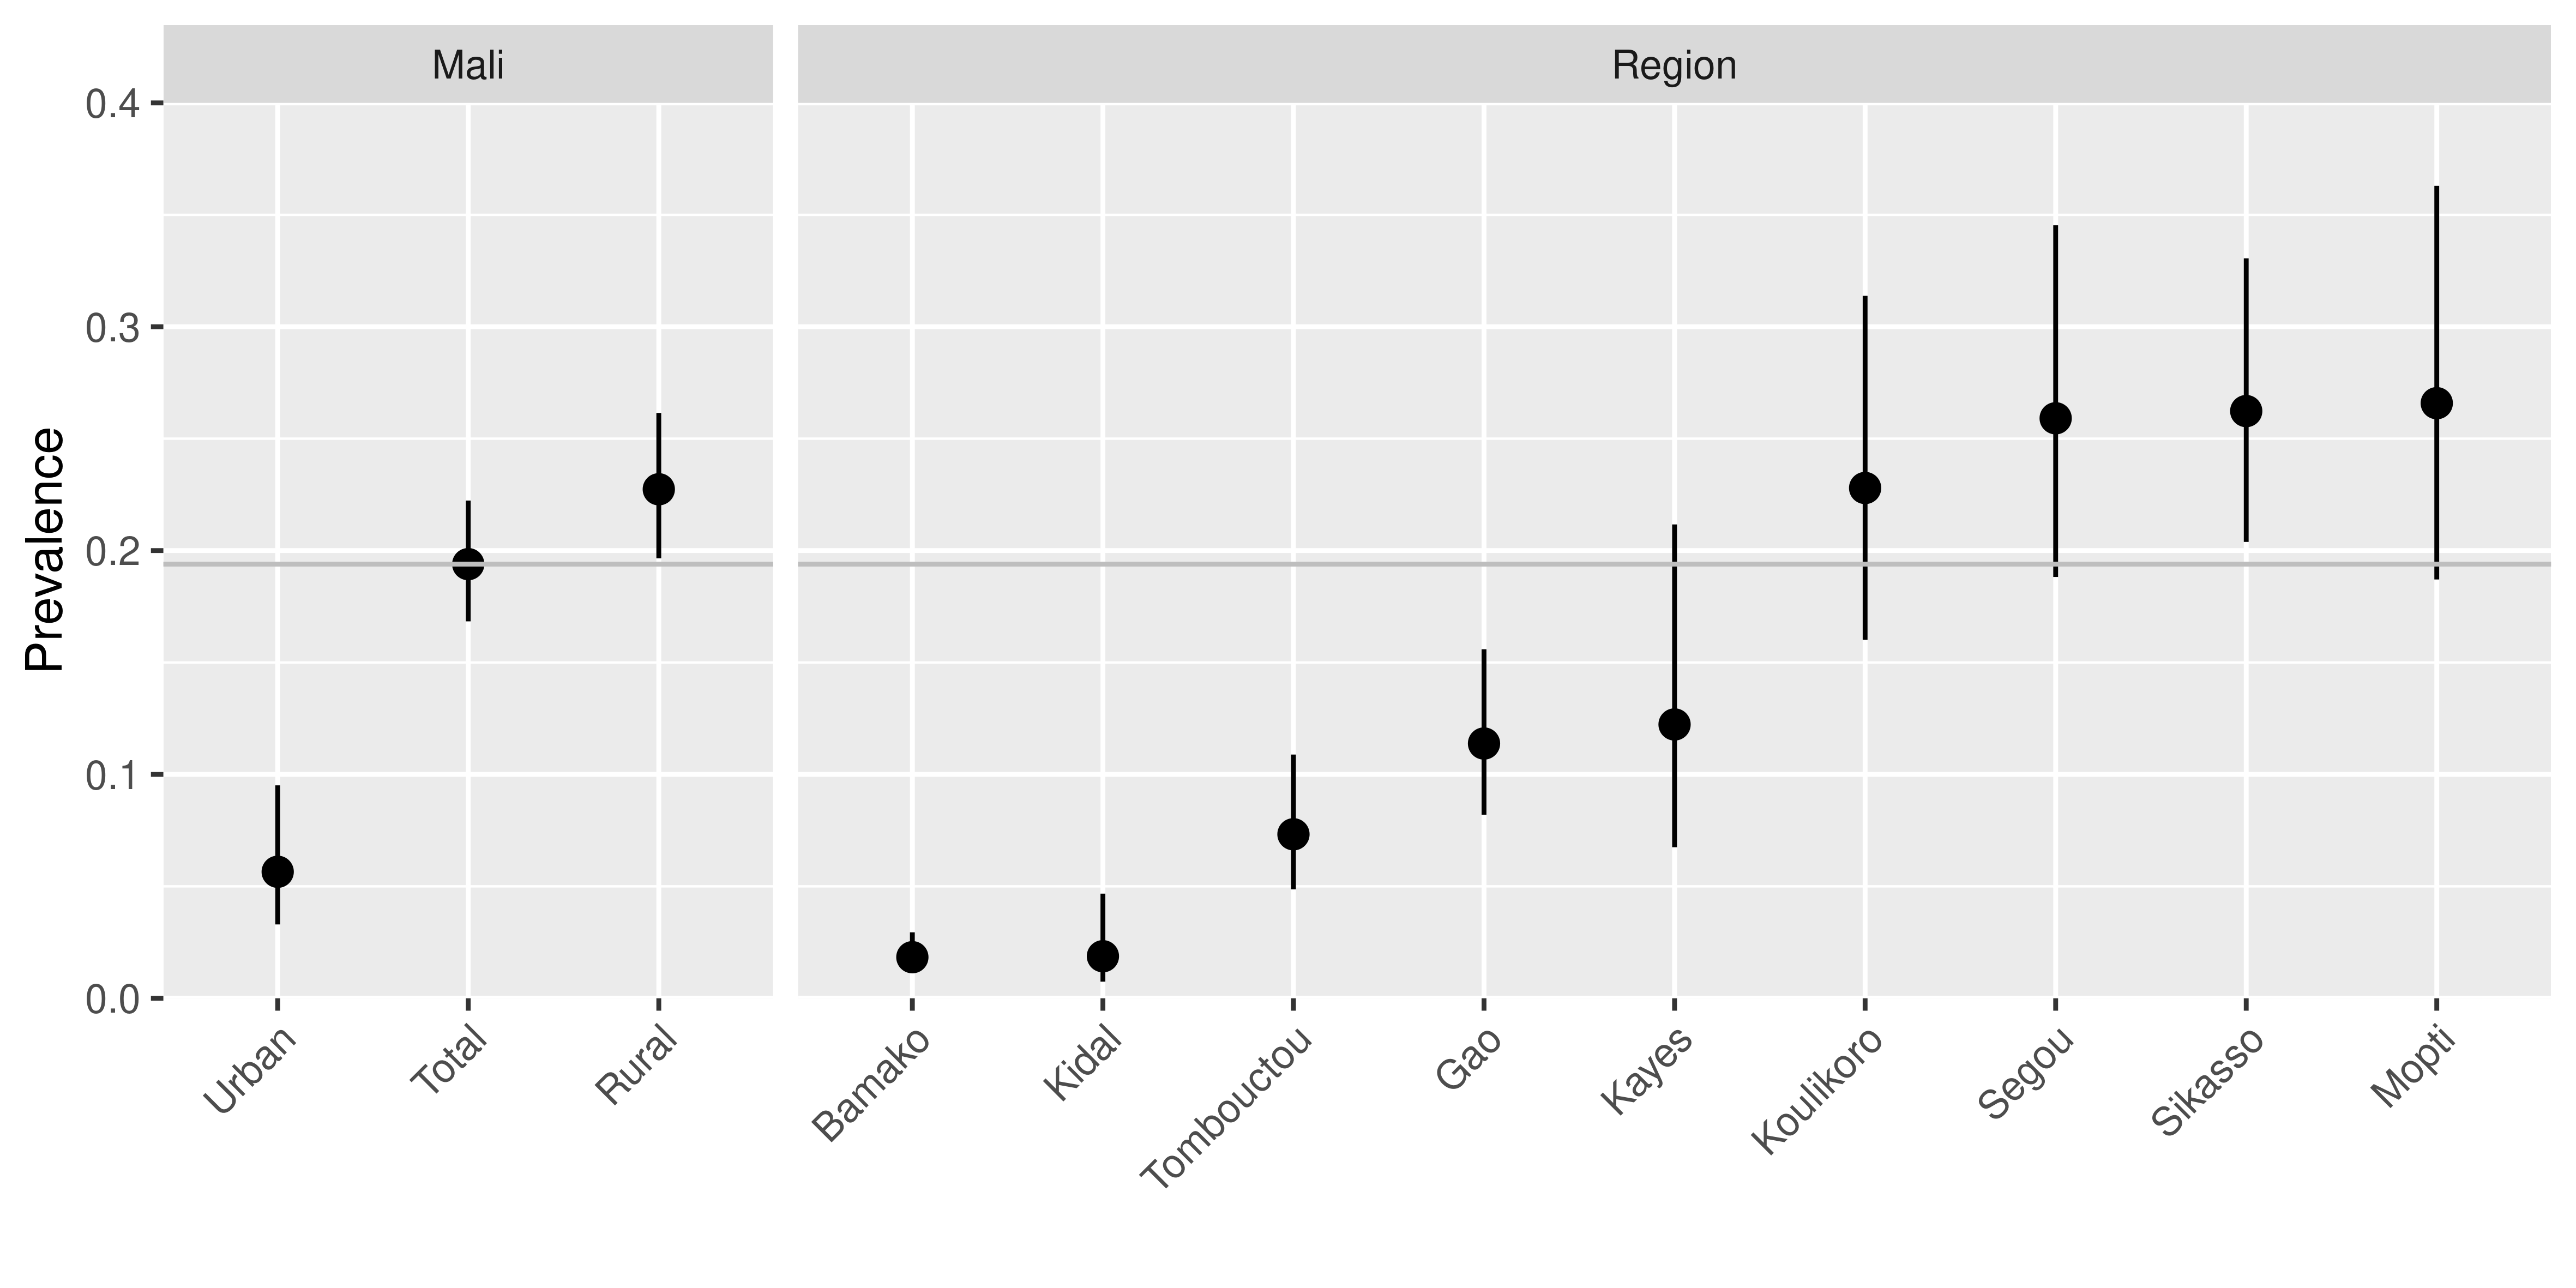
\includegraphics[width=0.9\textwidth, keepaspectratio]{figures/mali_designestimates.png}
	\caption{Geographic malaria risk in Mali: design-based estimates of malaria prevalence in children 6-59 months. Error bars indicate 95\% confidence intervals. Data from the Mali 2021 MIS.}
	\label{fig:mli_designestimates}
\end{figure}


\subsubsection*{Mali 2021 Malaria Indicator Survey}\label{sec:mali-2021-malaria-indicator-survey}

The Mali 2021 Malaria Indicator Survey (MIS) was designed to provide estimates of key malaria-related indicators at the national level, for urban and rural populations, and each of the eight administrative regions plus the capital Bamako. The latter is exclusively urban, yielding 17 strata (regions crossed with urbanicity). A total of 216 clusters were drawn from a sampling frame based on the 2009 population census. If the number of enumerated households per cluster surpassed 300, the area was partitioned and only one partition was selected for complete enumeration. In each, 26 households were selected randomly and all women (15-49) usually living in the selected households and present the night before the interview were eligible for the questionnaire. Additionally, all children aged 6-59 months were eligible for a rapid diagnostic test on malaria infection and anaemia \autocite{institutnationaldelastatistiqueinstatEnqueteIndicateursPaludisme2022}. 

\autoref{fig:mli_climatezones} shows the cluster locations of the Mali 2021 MIS. Northern Mali is characterised by a sparse and highly rural population. The realised survey cluster locations are therefore located predominantly in the south of the country. The design-based estimates and the corresponding confidence intervals of malaria prevalence in children 6-59 months are shown in \autoref{fig:mli_designestimates}. Strong subnational differences are discernible, both between regions as well as urban and rural designated areas. The urban-rural divide is particularly evident in the raw cluster-level prevalences. \autoref{fig:mli_scatterplot} plots the count of children who tested positive against the number of children in each cluster. Almost all urban clusters are below the 10\% line, and the rural clusters show much more variability in the raw estimates. Furthermore, even though the number of households sampled in each cluster is the same (26), the effective number of children tested per cluster varies greatly. In particular, any modelling strategy should account for different realised sample sizes at each cluster location. 

\begin{figure}[!t]
    \centering
    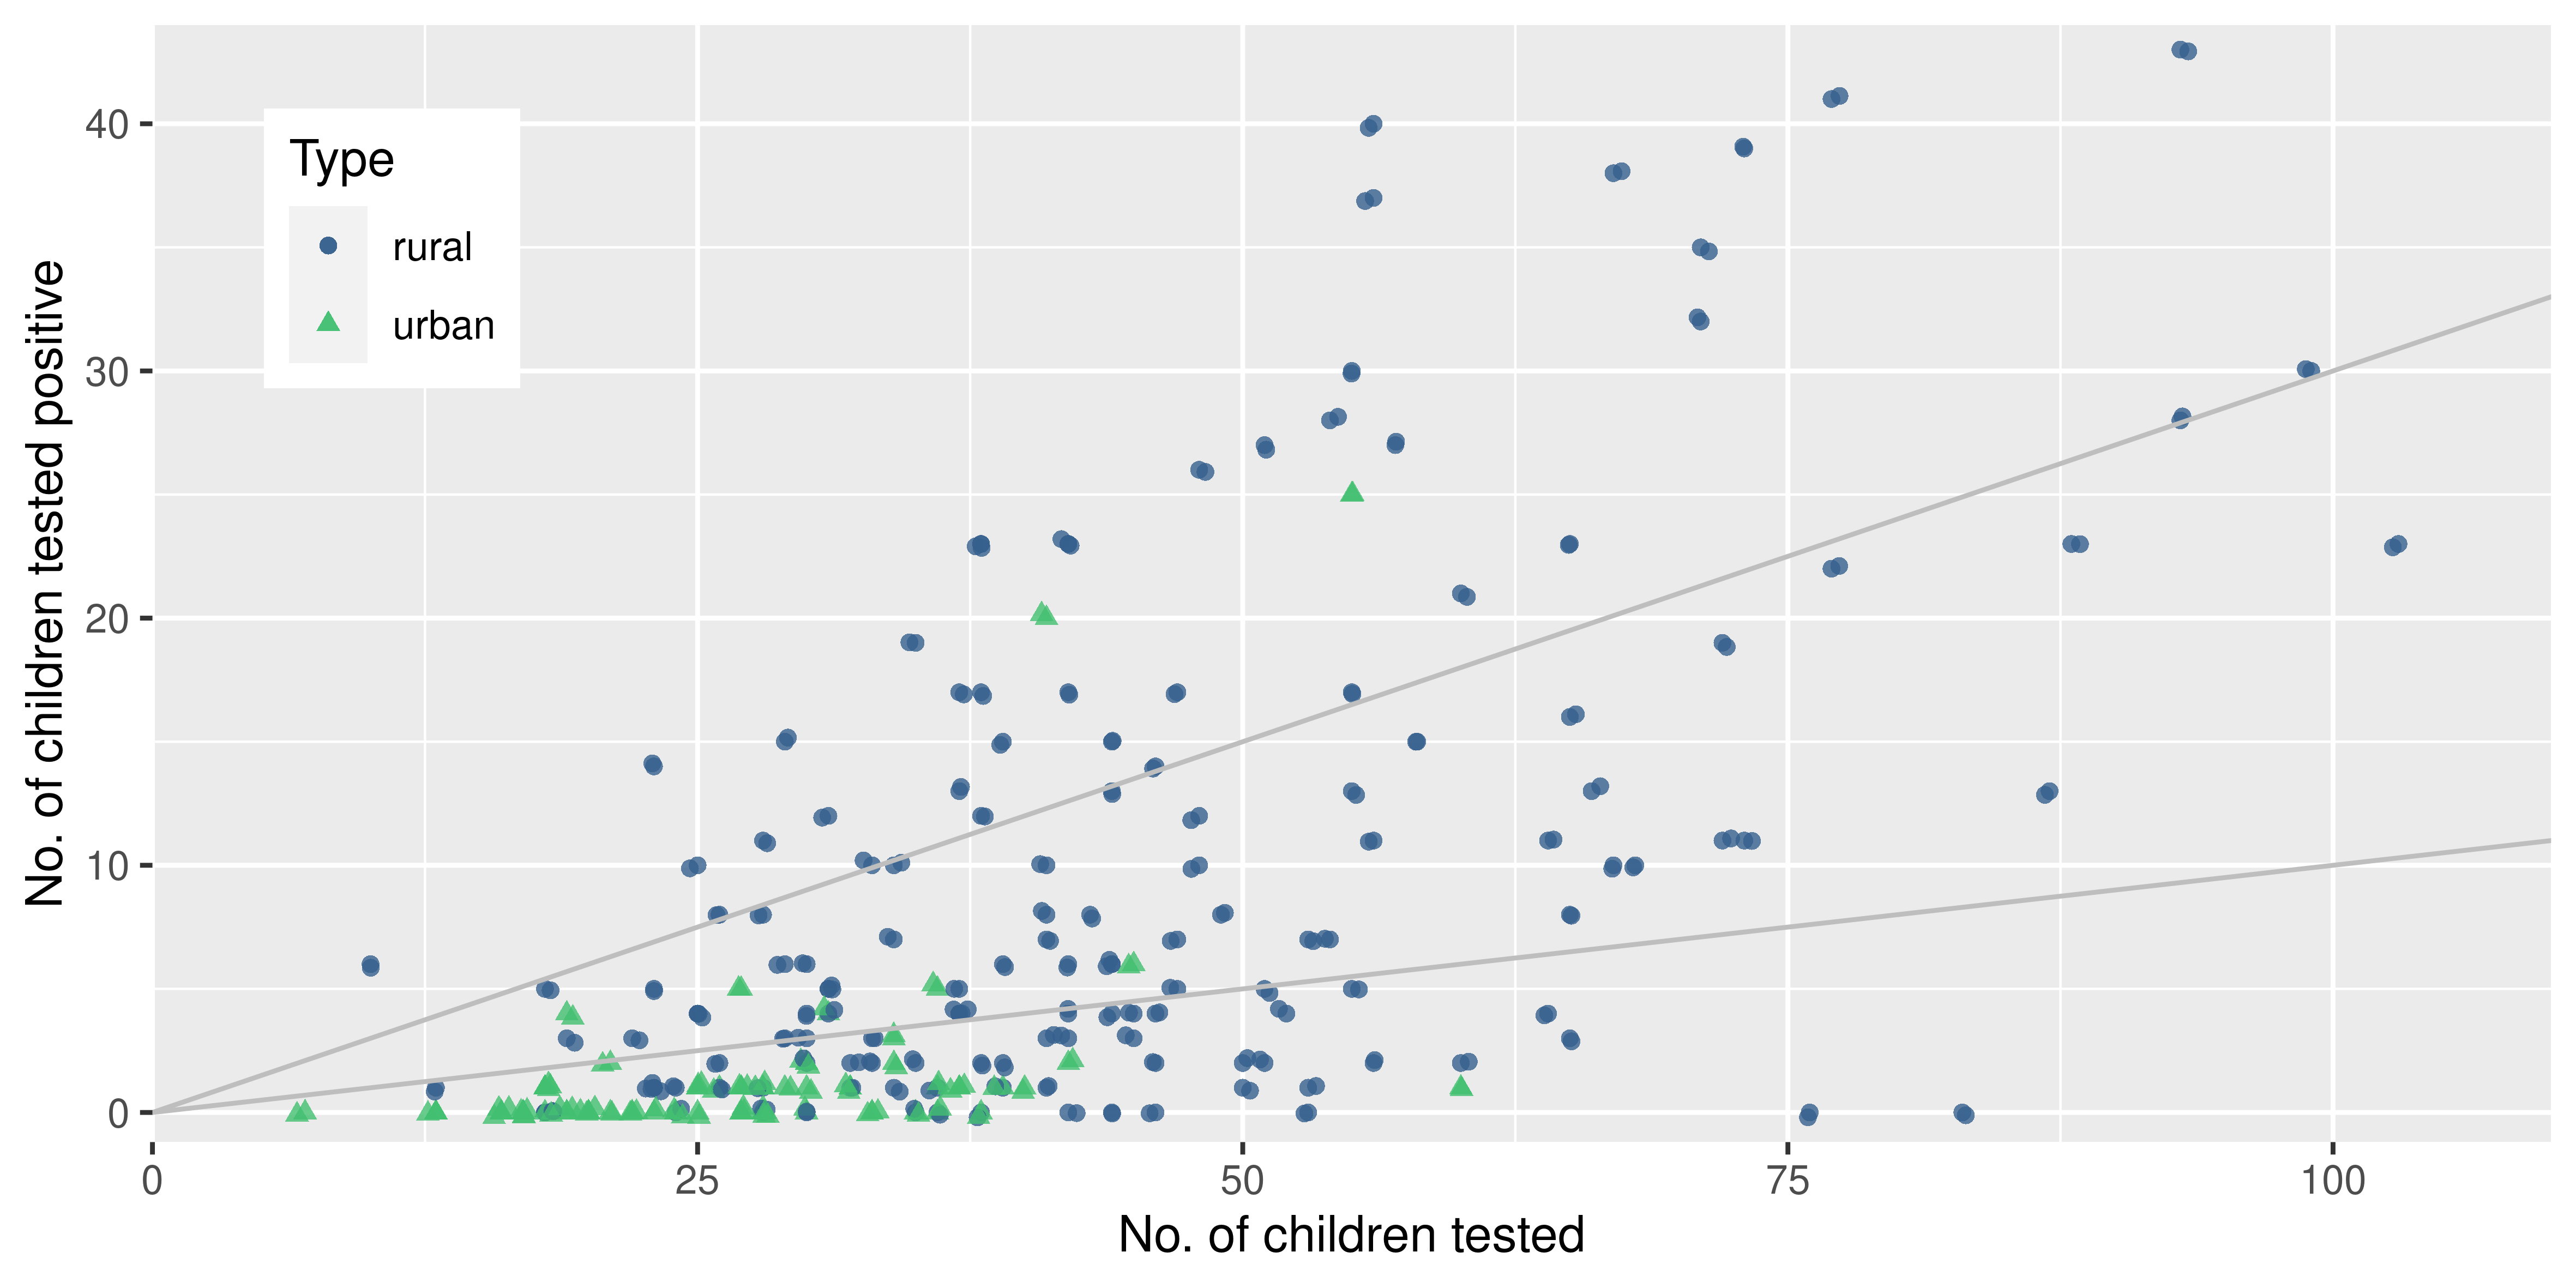
\includegraphics[width=0.9\textwidth, keepaspectratio]{figures/mali_scatterplot.png}
    \caption{Geographic malaria risk in Mali: number of children tested positive against cluster size. Grey lines indicate a raw prevalence of 30\% and 10\%, upper and lower lines, respectively. A small amount of noise was added to the values to enhance visualisation. Data from the Mali 2021 MIS.}
    \label{fig:mli_scatterplot}
\end{figure}


\subsubsection*{Environmental variables}

To inform local risk of malaria, the analysis includes environmental and climatic predictors that have been associated with malaria risk in previous work \autocite[see][and the references therein]{weissReexaminingEnvironmentalCorrelates2015, millarDetectingLocalRisk2018, weissMappingGlobalPrevalence2019, mohammedSpatialAnalysisClimatic2022}. Transmission risk is dependent on the species distribution of the \textit{Anopheles} mosquitoes, which are sensitive to climatic factors. The environmental variables for this case study are precipitation (annual aggregate) \autocite{funkClimateHazardsInfrared2015}, elevation (static) \autocite{jarvisHolefilledSRTMGlobe2008}, land surface temperature (annual mean, day and night) \autocite{didanMODISTerraVegetation2021b}. Additionally, I include two vegetation indices, the Enhanced Vegetation Index (EVI) and Normalised Difference Vegetation Index (NDVI) \autocite{wanMODISTerraLand2021}. 

As discussed in \textcite{dongModelingPresentationVaccination2021, paigeDesignModelBasedApproaches2022}, model-based approaches to small area estimation should include the stratification of the survey design, as omission may produce biased estimates. Therefore, to distinguish between urban and rural at unseen locations, I include an urban-rural indicator based on the degree of urbanisation from the Global Human Settlement Layers (GHSL) project \autocite{schiavinaGHSSMODR2022AGHS2022}. This variable is constructed based on estimated population counts and remotely sensed built-up grids.\footnote{An alternative approach was proposed in \textcite{dongModelingPresentationVaccination2021} and \textcite{paigeDesignModelBasedApproaches2022}, where the authors construct an urbanicity variable with information about the sampling frame published in the survey reports. The surveys publish the percentage of urban population for each region and the country from the used primary sampling frame, and with population density layers, a threshold to obtain an urban-rural indicator per grid cell can be inferred. In the case of Mali, this resulted in very few urban locations. Ultimately, both approaches are likely sensitive to the chosen population density layer, which has been shown to induce substantial differences in applications \autocite[see, for example, ][]{hierinkDifferencesGriddedPopulation2022a}. For further discussion on the modelling of urban-rural fractions, and a comparison of alternative approaches, see \textcite{wuModelingUrbanRural2022}.} Lastly, I include population counts \autocite{schiavinaGHSPOPR2022AGHS2022} and the climate classification by Köppen-Geiger \autocite{beckPresentFutureKoppenGeiger2018}. Mali is covered by three distinct climate regions, see \autoref{fig:mli_climatezones}.

\begin{figure}[!t]
	\centering
	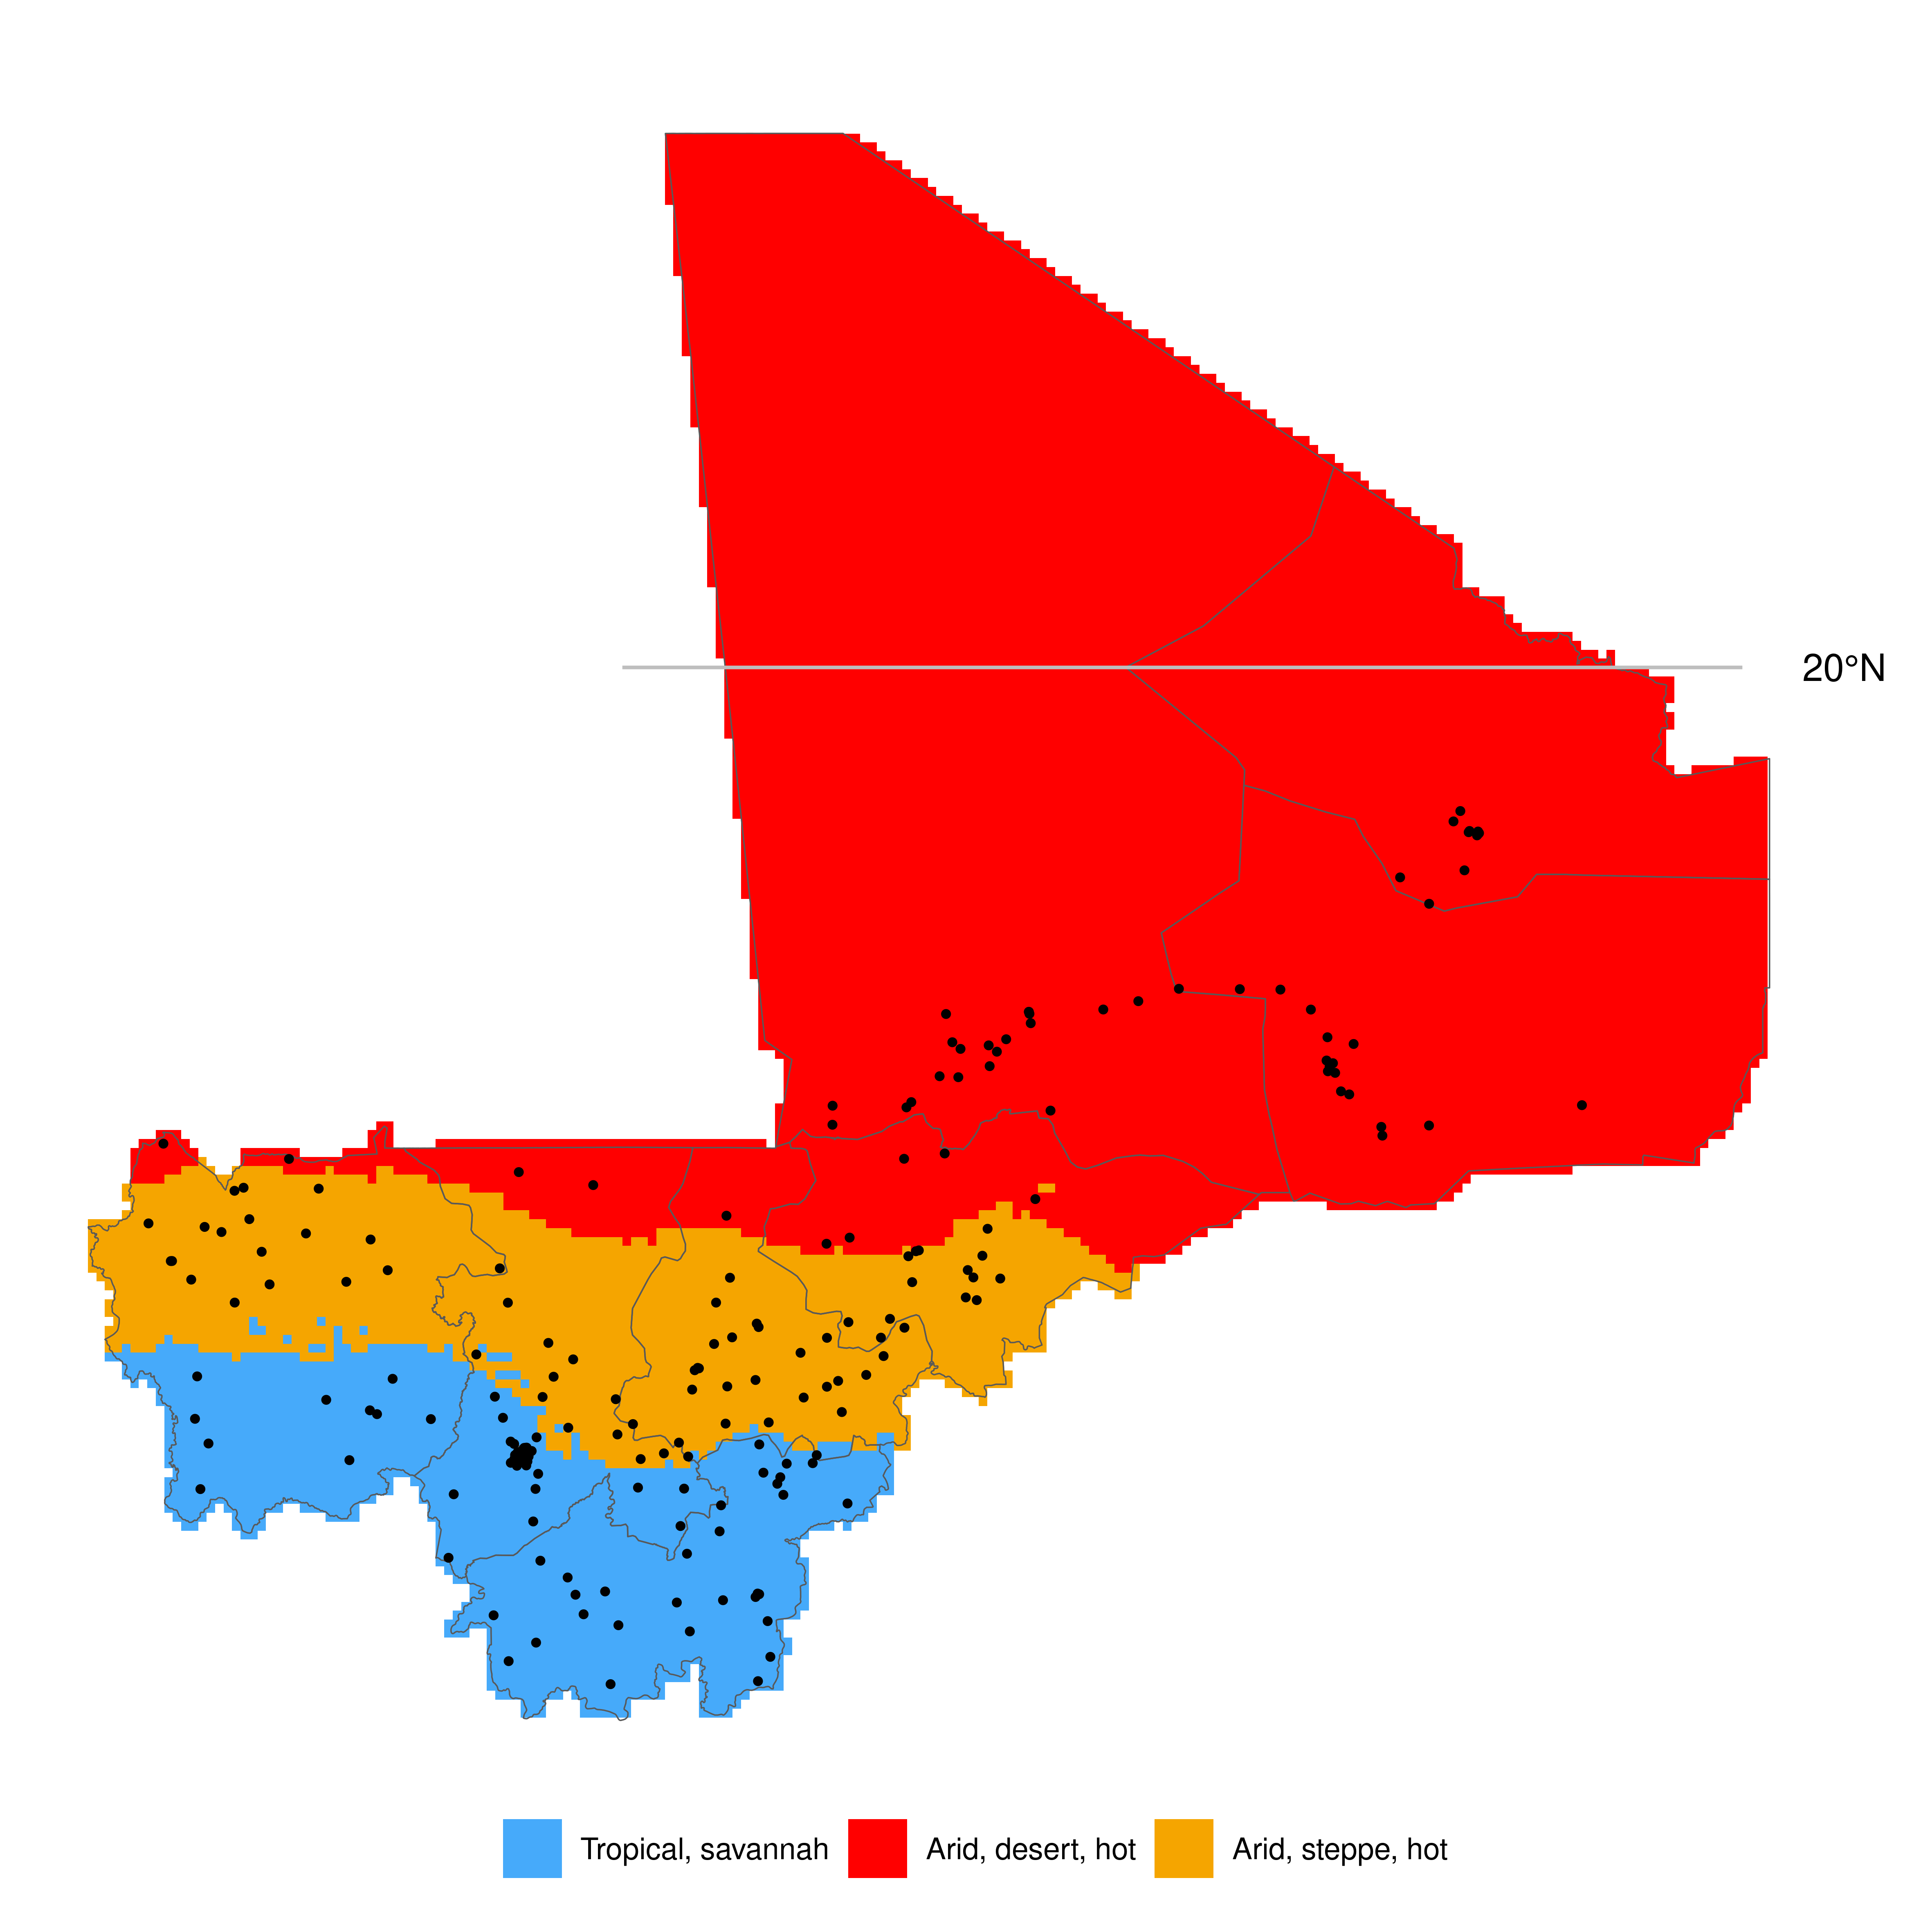
\includegraphics[width=0.9\textwidth, keepaspectratio]{figures/mali_climatezones.png}
	\caption{Geographic malaria risk in Mali: climate classification by Köppen Geiger and survey cluster locations from the Mali 2021 MIS. Regions north of the $20^\circ$ degree are omitted due to data sparsity.}
	\label{fig:mli_climatezones}
\end{figure}


\subsubsection*{Matching georeferenced data}

For each cluster, the locations of the interviewed households are recorded and the centroid is taken as cluster-level information. To ensure the privacy of the respondents, a randomisation procedure is applied to the coordinates, where urban locations are randomly displaced up to 2km and rural up to 5km with an additional 1\% of the observations up to 10km \autocite{burgertGeographicDisplacementProcedure2013}. This naturally introduces measurement error and mismatching when integrated with other data sources based on the geographic location.\footnote{In and of itself, there is not much to be done to counter this induced error. \textcite{wuModelingUrbanRural2022} discuss a Bayesian approach to account for the displacement of urban regions. \textcite{michlerPrivacyProtectionMeasurement2022} assesses the impact of different spatial anonymisation techniques for a similar series of household surveys from the World Bank. Comparing estimates of measures of agricultural productivity for rural and agricultural households, the authors conclude the anonymisation method introduces limited error, but care should be taken in the selection of remote sensing products. In this case study, I take the cluster locations as provided.} Additional information on the data and the matching procedure is given in the supplementary material.


\subsection{Modelling}

\subsubsection*{Model specification}

From the survey micro-data, one obtains for each cluster $c$ a count of children $n_c$ that were tested, and a count $y_c$ that tested positive. A natural way to model such data is with a Binomial likelihood in a generalised additive model framework. To estimate the model, I use the component-wise boosting approach described herein. Thus, let
\begin{equation*}
	y_c \sim \Binomial(n_c, \mu_c), \quad c = 1, \dots, N.
\end{equation*}  
The relative probability of occurrence $\mu_c$ is estimated with a linear predictor 
\begin{align}\label{eq:mli_main}
	\begin{split}
	\logit(\mu_c)   &= \eta_c \\
	                &= \beta_0  + \sum_{j = 1}^{p} \beta_j x_{jc} + \sum_{k = 1}^{q} f_{\mathtt{smooth}} (x_{kc}) + f_{\mathtt{spatial}} (x_{\text{lon}, c}, x_{\text{lat}, c}), \quad c = 1, \dots, n.
	\end{split}
\end{align}
The loss function is taken to be the negative log-likelihood of the binomial distribution. In this base model, I include linear effects for the categorical variable (urbanicity) and smooth effects using cubic P-splines with second-order differences and 20 inner knots. To ensure unbiased effect selection these are included in the parametric and centred decomposition discussed before. To account for spatial effects, I include a bivariate smooth with a similar decomposition. For details see \textcite{kneibVariableSelectionModel2009}.

As discussed in \textcite{dongModelingPresentationVaccination2021}, count data aggregated to cluster-level often exhibit more variability than be accounted for in a binomial response distribution. The data is said to be \textit{overdispersed}. To accommodate possible within-cluster variation, the authors suggest a beta-binomial likelihood
\begin{equation*}
	y_c \sim BB(n_c, \mu_c, \sigma_c), \quad c = 1, \dots, N.
\end{equation*} 

The beta-binomial distribution can be thought of first drawing a probability from the beta distribution $p_c \sim \Beta(\mu_c, \sigma_c)$ and then the cluster-level count $y_c \sim \Binomial(n_c, p_c)$. Hence, it accommodates greater variability in the data than the binomial distribution. For $\sigma \rightarrow 0$ the limiting distribution is the binomial distribution, hence greater values of $\sigma_c$ correspond to a higher degree of overdispersion. Additional information on the response distributions is included in the supplementary material.

The beta-binomial distribution can be modelled in a boosting framework by moving to the distributional regression approach, which allows additive predictors for both the mean and the degree of overdispersion (i.e., the location and shape of the distribution). Thus, let $\eta_{\mu, c}$ be the predictor defined in \autoref{eq:mli_main} and 
\begin{align}
	\begin{split}
		\log(\sigma_c) & = \eta_{\sigma, c}\\
		& = \beta_0 + \beta_1 x_{\mathtt{urban}}, \quad c = 1, \dots, N.
	\end{split}
\end{align}
Although it would be simple to add additional terms to model the degree of overdispersion of the conditional distribution, an intercept and urbanicity keeps model complexity low and are motivated by the urban-rural divide. 

Besides the comparison of the two different choices of the data model, I consider alternative specifications of the additive predictor for the beta-binomial model. First, a simple linear model as a baseline. Two versions of the linear model, one augmented with a bivariate spatial smooth, and a second specification of the linear model augmented with the spatial effect and all linear covariates interacted with the climate classification. I also consider a model with spatially-varying coefficients, where each continuous covariate enters the additive predictor linearly, as a modifier of a bivariate smooth. Finally, as an alternative to the pre-specified semi-parametric effects, I also evaluate the performance of regression trees as base learners with a maximum interaction depth of 4 and with all other parameters left at their default values.\footnote{It would be interesting to see if the fully nonparametric specification could be further improved by the use of oblique coordinates \autocite{mollerObliqueGeographicCoordinates2020}.}

I employ a bootstrap approach to quantify variability in the estimated effects. To make ideal use of the data I draw bootstrap samples from the individual-level data stratified by cluster. The model is refitted and the estimates are compared to the 'main' model, the model fitted on the original data set.

\begin{table}[!t]

	\begin{tabularx}{\textwidth}{Xrrrrrr}

	Model & Bias & MAE & RMSE & 80\% PI & 90\% PI & 95\% PI \\ \arrayrulecolor{black!30}\midrule

	Beta binomial & -0.005 & 0.093 & 0.131 & 0.861 & 0.944 & 0.963 \\ 
	Binomial & -0.007 & 0.091 & 0.131 & 0.597 & 0.708 & 0.759 \\ 
	
	\end{tabularx}
	
	\caption{Geographic malaria risk in Mali: model validation based on 10-fold cross-validation stratified by survey region. Values rounded rounded to the nearest hundredth.}
	\label{tab:mali_modelvalidation}
	
\end{table}

\subsubsection*{Model evaluation and selection}

Given the lower sample size ($N = 216$), the holdout method is not reasonable and I select the number of boosting iterations based on where the minimum of the cross-validated risk is attained. Cross-validation estimates are based on $K=10$ and folds are stratified by region, as the number of clusters per strata does not allow for stratification by survey design strata. The step-length $\nu$ is fixed at $0.1$.

To compare the different model specifications proposed above, I employ nested cross-validation. The outer loop consists of 10-fold cross-validation, and the inner loop for early stopping is likewise based on 10-fold cross-validation both stratified by survey regions. First, I validate the data model for the prevalence data.  \autoref{tab:mali_modelvalidation} displays three common regression evaluation metrics for the point predictions, that is Bias, Mean Absolute Error (MAE), and Root Mean Squared Error (RMSE). To assess the quality of the prediction intervals, I also include the average coverage of the $100(1-\alpha)$\% prediction interval (PI) based on the conditional distribution. The $100(1-\alpha)$\% PI is defined as
\begin{equation*}
	PI_{1-\alpha}(x) = \left[Q_{\alpha / 2}(x), Q_{1-\alpha / 2}(x)\right]
\end{equation*}
where $Q_{\alpha}$ is the $\alpha$-quantile of the conditional distribution. Bias, MAE and RMSE are calculated with respect to the target of inference $\hat{\mu_c}$ and the raw prevalence at cluster-level $y_c / n_c$, and the coverage of the PI is calculated at the observed counts. The presented results are the average values over the outer hold-out folds.

Concerning the first three metrics, the three models show only minor differences. All tend to slightly overestimate the observed rate (bias). Given that the comparison is only based on 10-folds with a comparatively small sample size of 216 clusters, the differences should be considered marginal. However, that is not the case for the coverage of the prediction intervals. Here the binomial model does markedly worse than the model with the beta-binomial likelihood. Where the 90\% PIs only cover on average around 70 \% of the observations, the beta-binomial achieves a coverage above 90\%. Clearly, the prevalence data show more variability than can be accommodated in the binomial distribution, indicating the beta-binomial model has a superior fit. The following results, therefore, are based on the data models with the beta-binomial model.

\begin{figure}[!t]
	\centering
	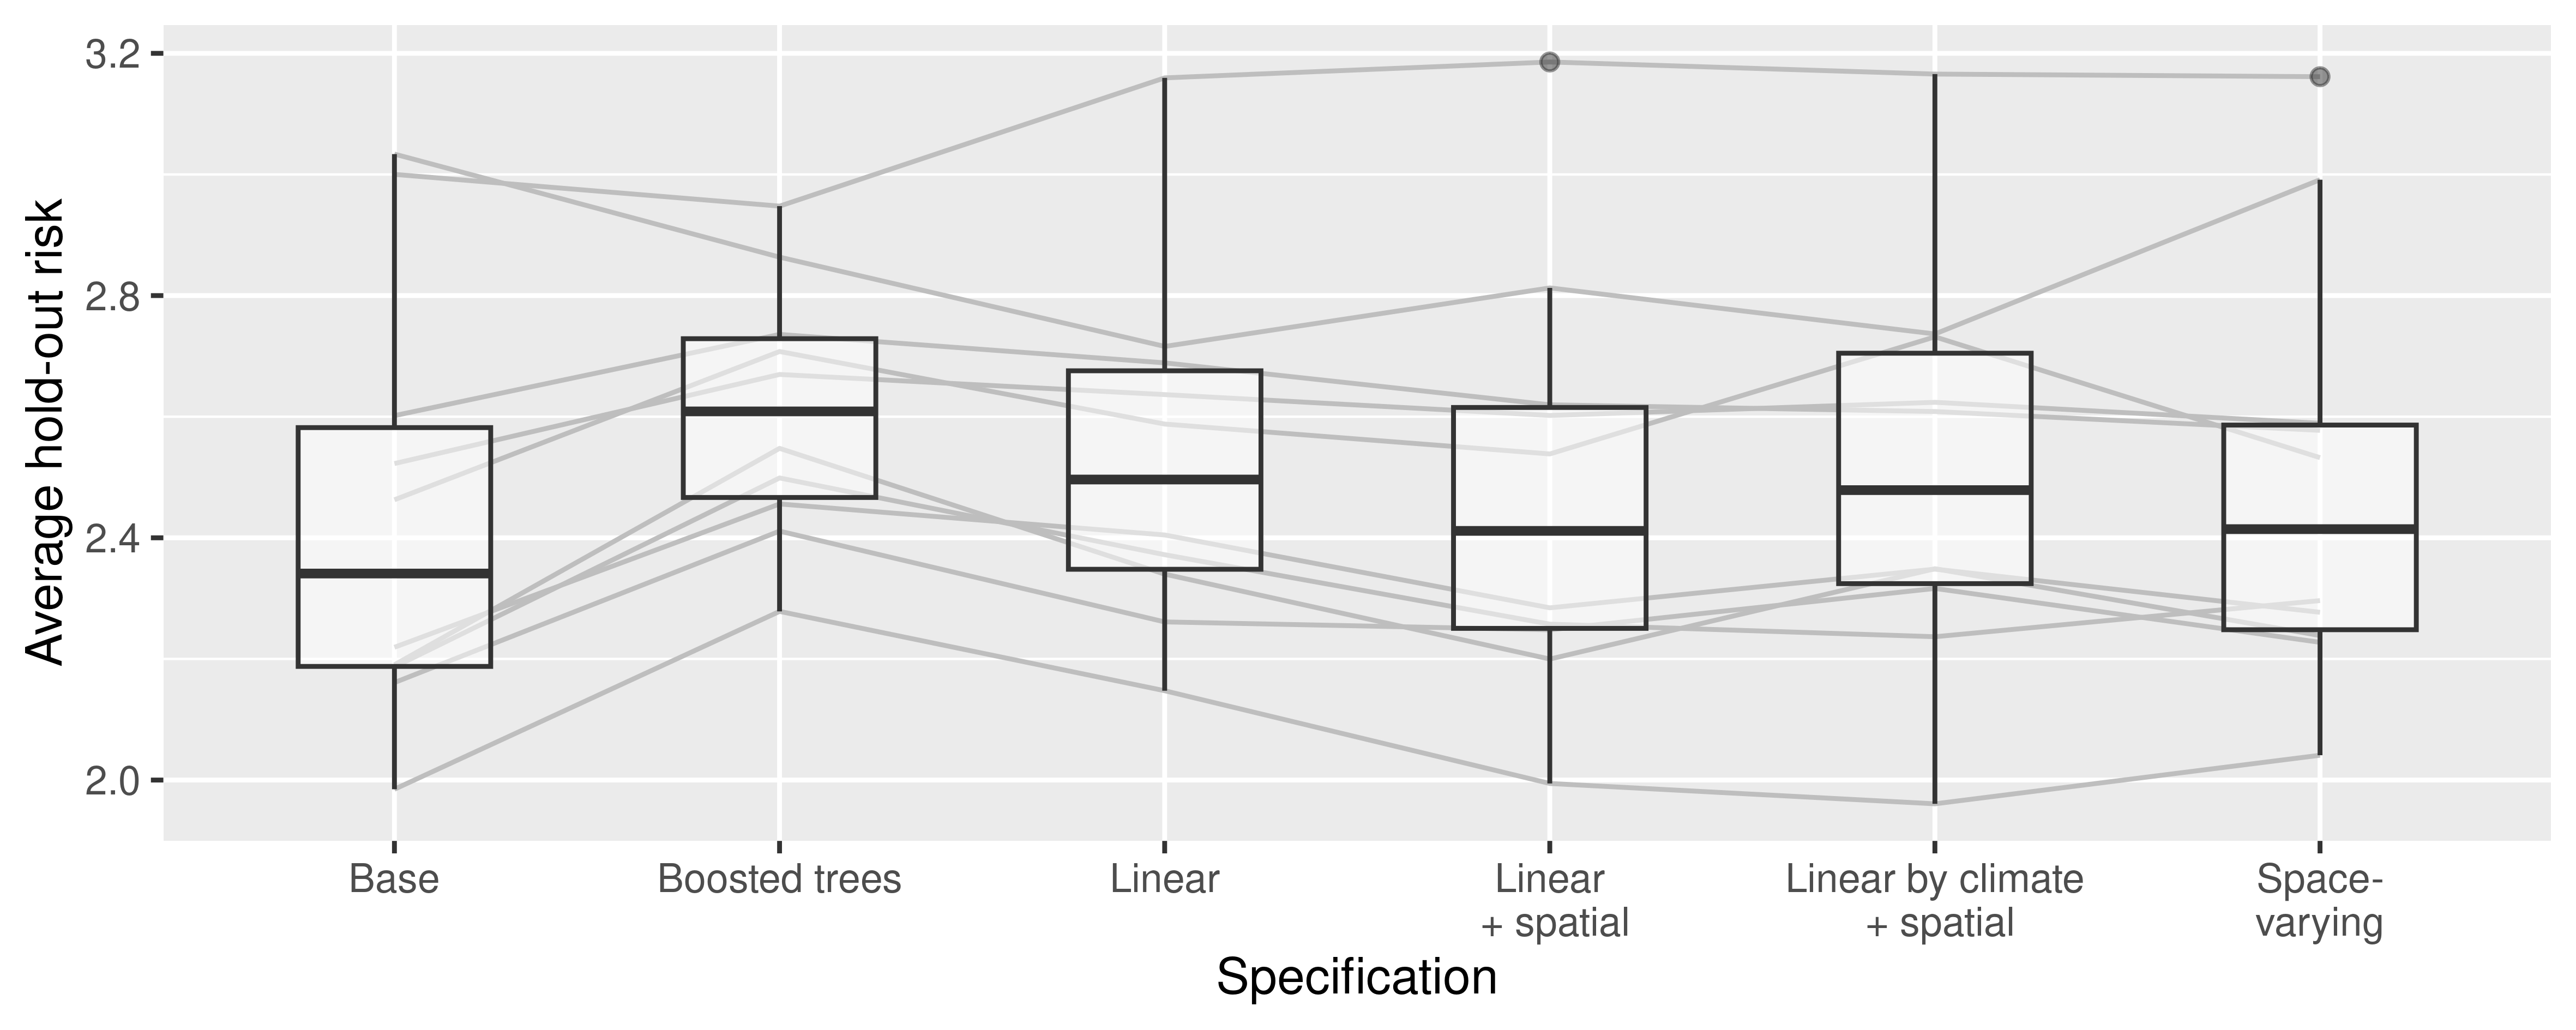
\includegraphics[width=0.9\textwidth, keepaspectratio]{figures/mali_modelselection.png}
	\caption{Geographic malaria risk in Mali: comparison of different model specifications. Lower is better. Grey lines indicate the average hold-out risk of 10-fold cross-validation stratified by survey regions.}
	\label{fig:mali_modelselection}
\end{figure}

Next, \autoref{fig:mali_modelselection} provides the comparison of the hold-out risk of the alternative model specifications. Clearly, likely due to the data limitations, the variability in the generalisation performance is high. Interestingly, the plain linear model does provide a tenable baseline, and the addition of a spatial effect tends to improve holdout risk. Augmenting the model with interactions by the climatological zone introduces instability. Interestingly, boosted trees fare the worst in this comparison, but with less variability. Overall, the base specification as in \autoref{eq:mli_main} provides the best generalisation performance. Based on this model, I will discuss the estimated factors and grid-cell predictions below.


\subsection{Results}

\autoref{fig:mali_categoricaleffects} shows the coefficients of the categorical covariates included in the model. Note that there -- as for all the following partial effect estimates -- the estimates are provided on the scale of the link function. Thus, for the conditional mean the partial effects are on the log-odds ratio of $\mu$, and for the conditional scale of the beta-binomial distribution on the $\log$ scale of $\sigma$.\footnote{Note, the effects of ecological covariates should not be interpreted on an individual level, as one risks to commit an ecological fallacy \autocite{piantadosiEcologicalFallacy1988}.}

\begin{figure}[!t]
	\centering
	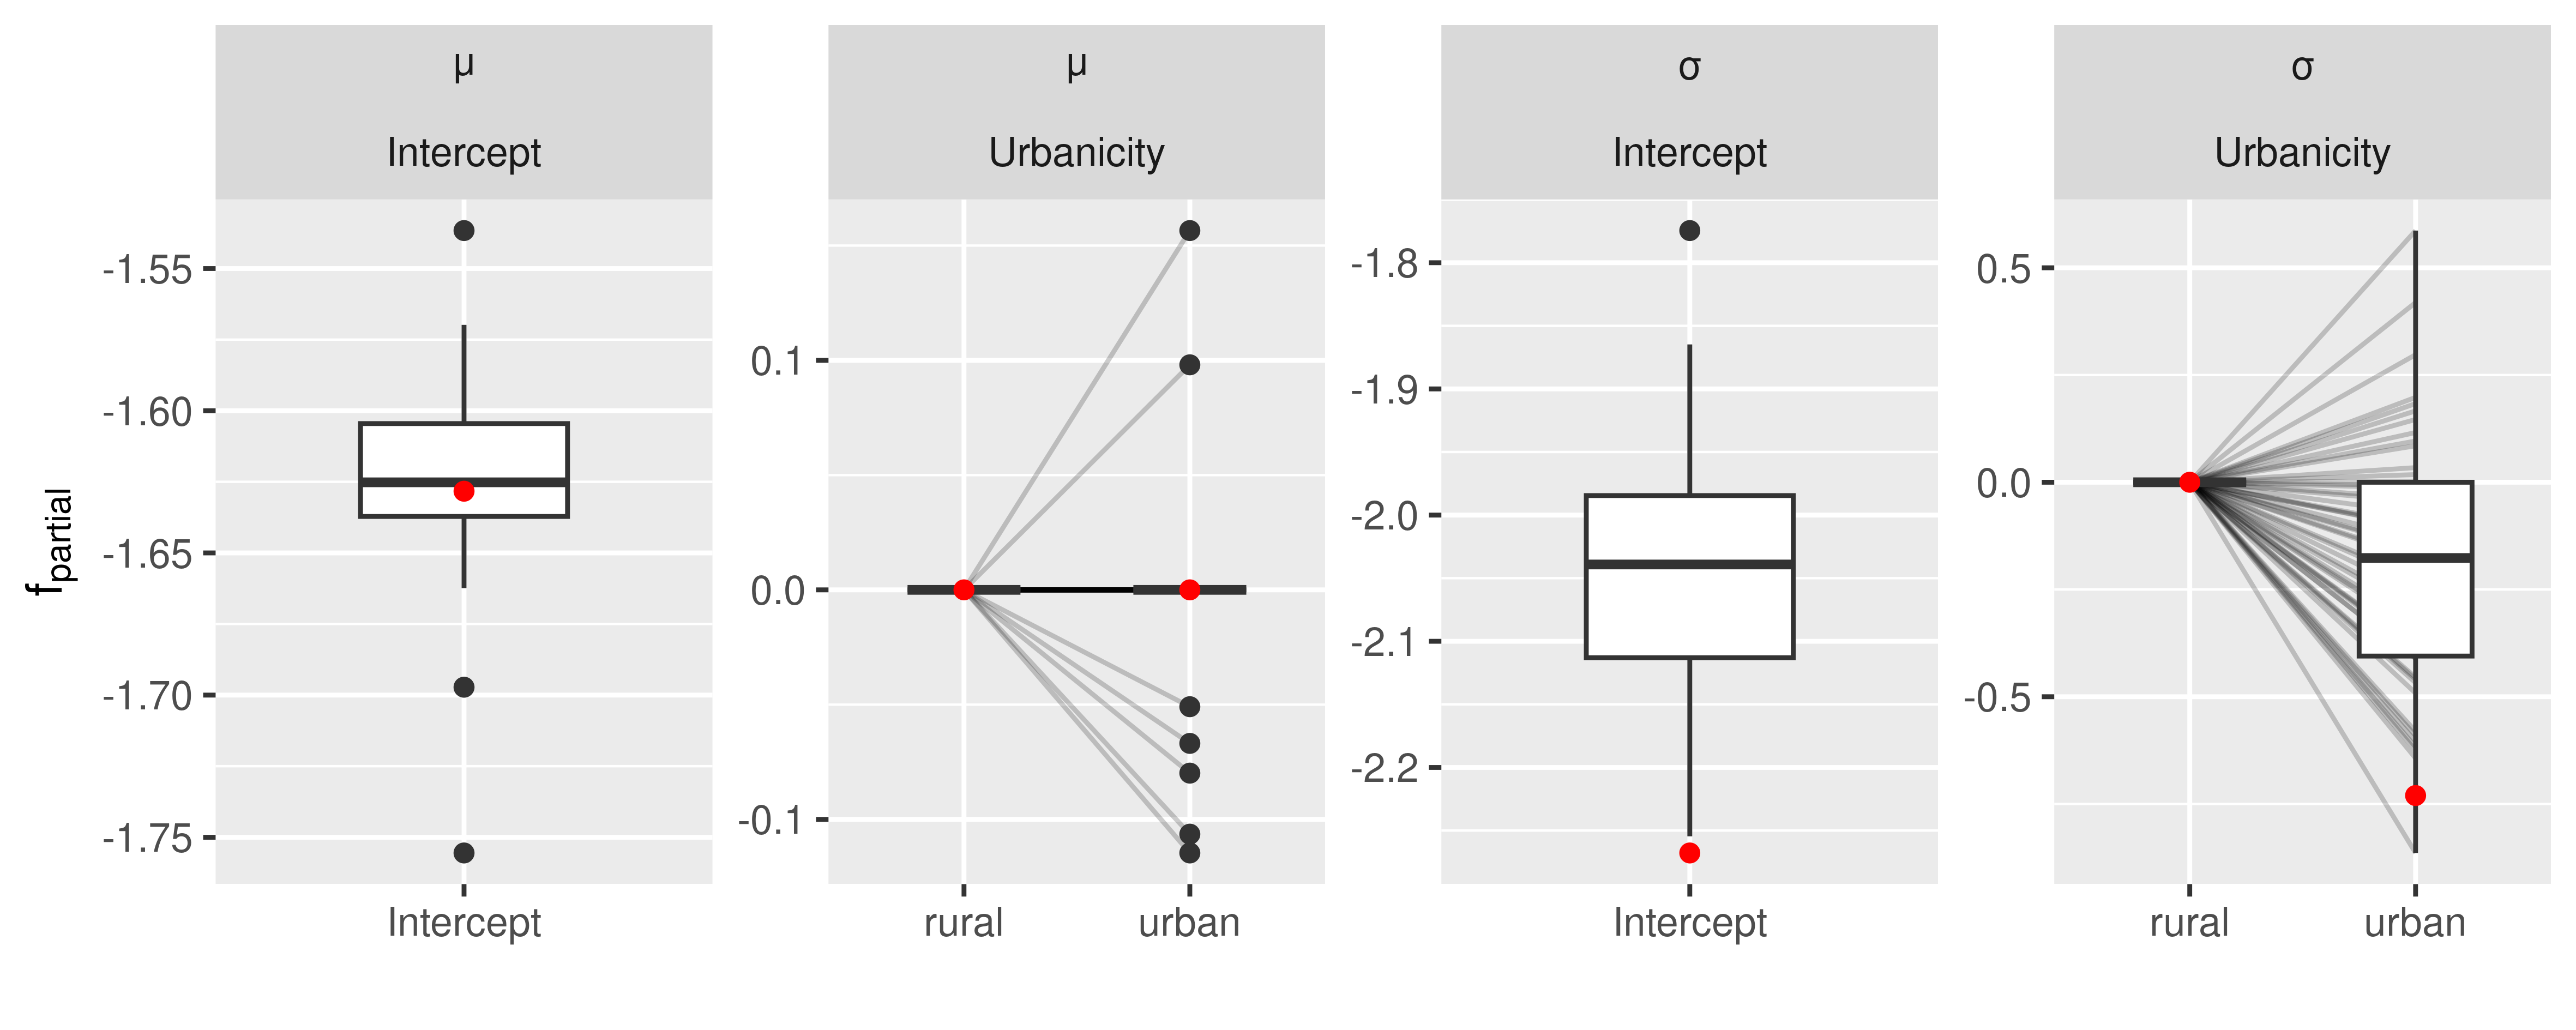
\includegraphics[width=0.9\textwidth, keepaspectratio]{figures/mali_categoricaleffects.png}
	\caption{Geographic malaria risk in Mali: estimated coefficients of the intercept and urbanicity covariate. The red points indicate the estimated effect of the main model and boxplots the empirical distribution of the estimated coefficients over the 50 bootstrap samples.}
	\label{fig:mali_categoricaleffects}
\end{figure}

For $\mu$, urbanicity is estimated to be zero in the main model, with a few deviations in the bootstrap samples. For $\sigma$, the urbanicity coefficient is estimated to be negative, with the third quartile below zero. 

\autoref{fig:mli_main_effects} plots the partial effects of the continuous covariates. The main model is indicated by the red line, and the models replicated on 50 bootstrap samples are shown in the background. For elevation, the estimated effect is linear, higher altitudes correspond to a decreased malaria risk. The Enhanced Vegetation Index (EVI) is estimated clearly in a U-shaped form, in particular, an increased risk towards the upper end of the scale. This is in line with the interpretation of the index, where higher values indicate dense vegetation. Likewise, the Normalised Vegetation Index (NDVI) shows an increased risk for higher values and can be interpreted similarly. The effect of land surface temperature during the day is mostly estimated to be zero, as in the main model, with only some bootstrap replicates showing different results. For the temperature at night, the effect is estimated to be negatively associated with malaria risk in the lower range, peaking between 20--22 degrees and declining for higher values. For values toward $26^\circ$, it shows an up-tick, but not indistinguishable from zero. The (log) population counts are relatively flat for the first half of the support then drastically decrease, i.e., higher population counts are associated with a lower risk of malaria. Since a higher population equate with urban areas, this is plausible. The annual aggregated precipitation shows an increasing effect up until 600, then decrease. For values beyond 1200, the estimation is supported by few data points (as indicated by the rug plot), correspondingly, the estimates show much more variability. Again, the effect selection properties of the component-wise boosting algorithm yield informative selections about the functional form of a given covariate.

\begin{figure}[!t]
	\centering
	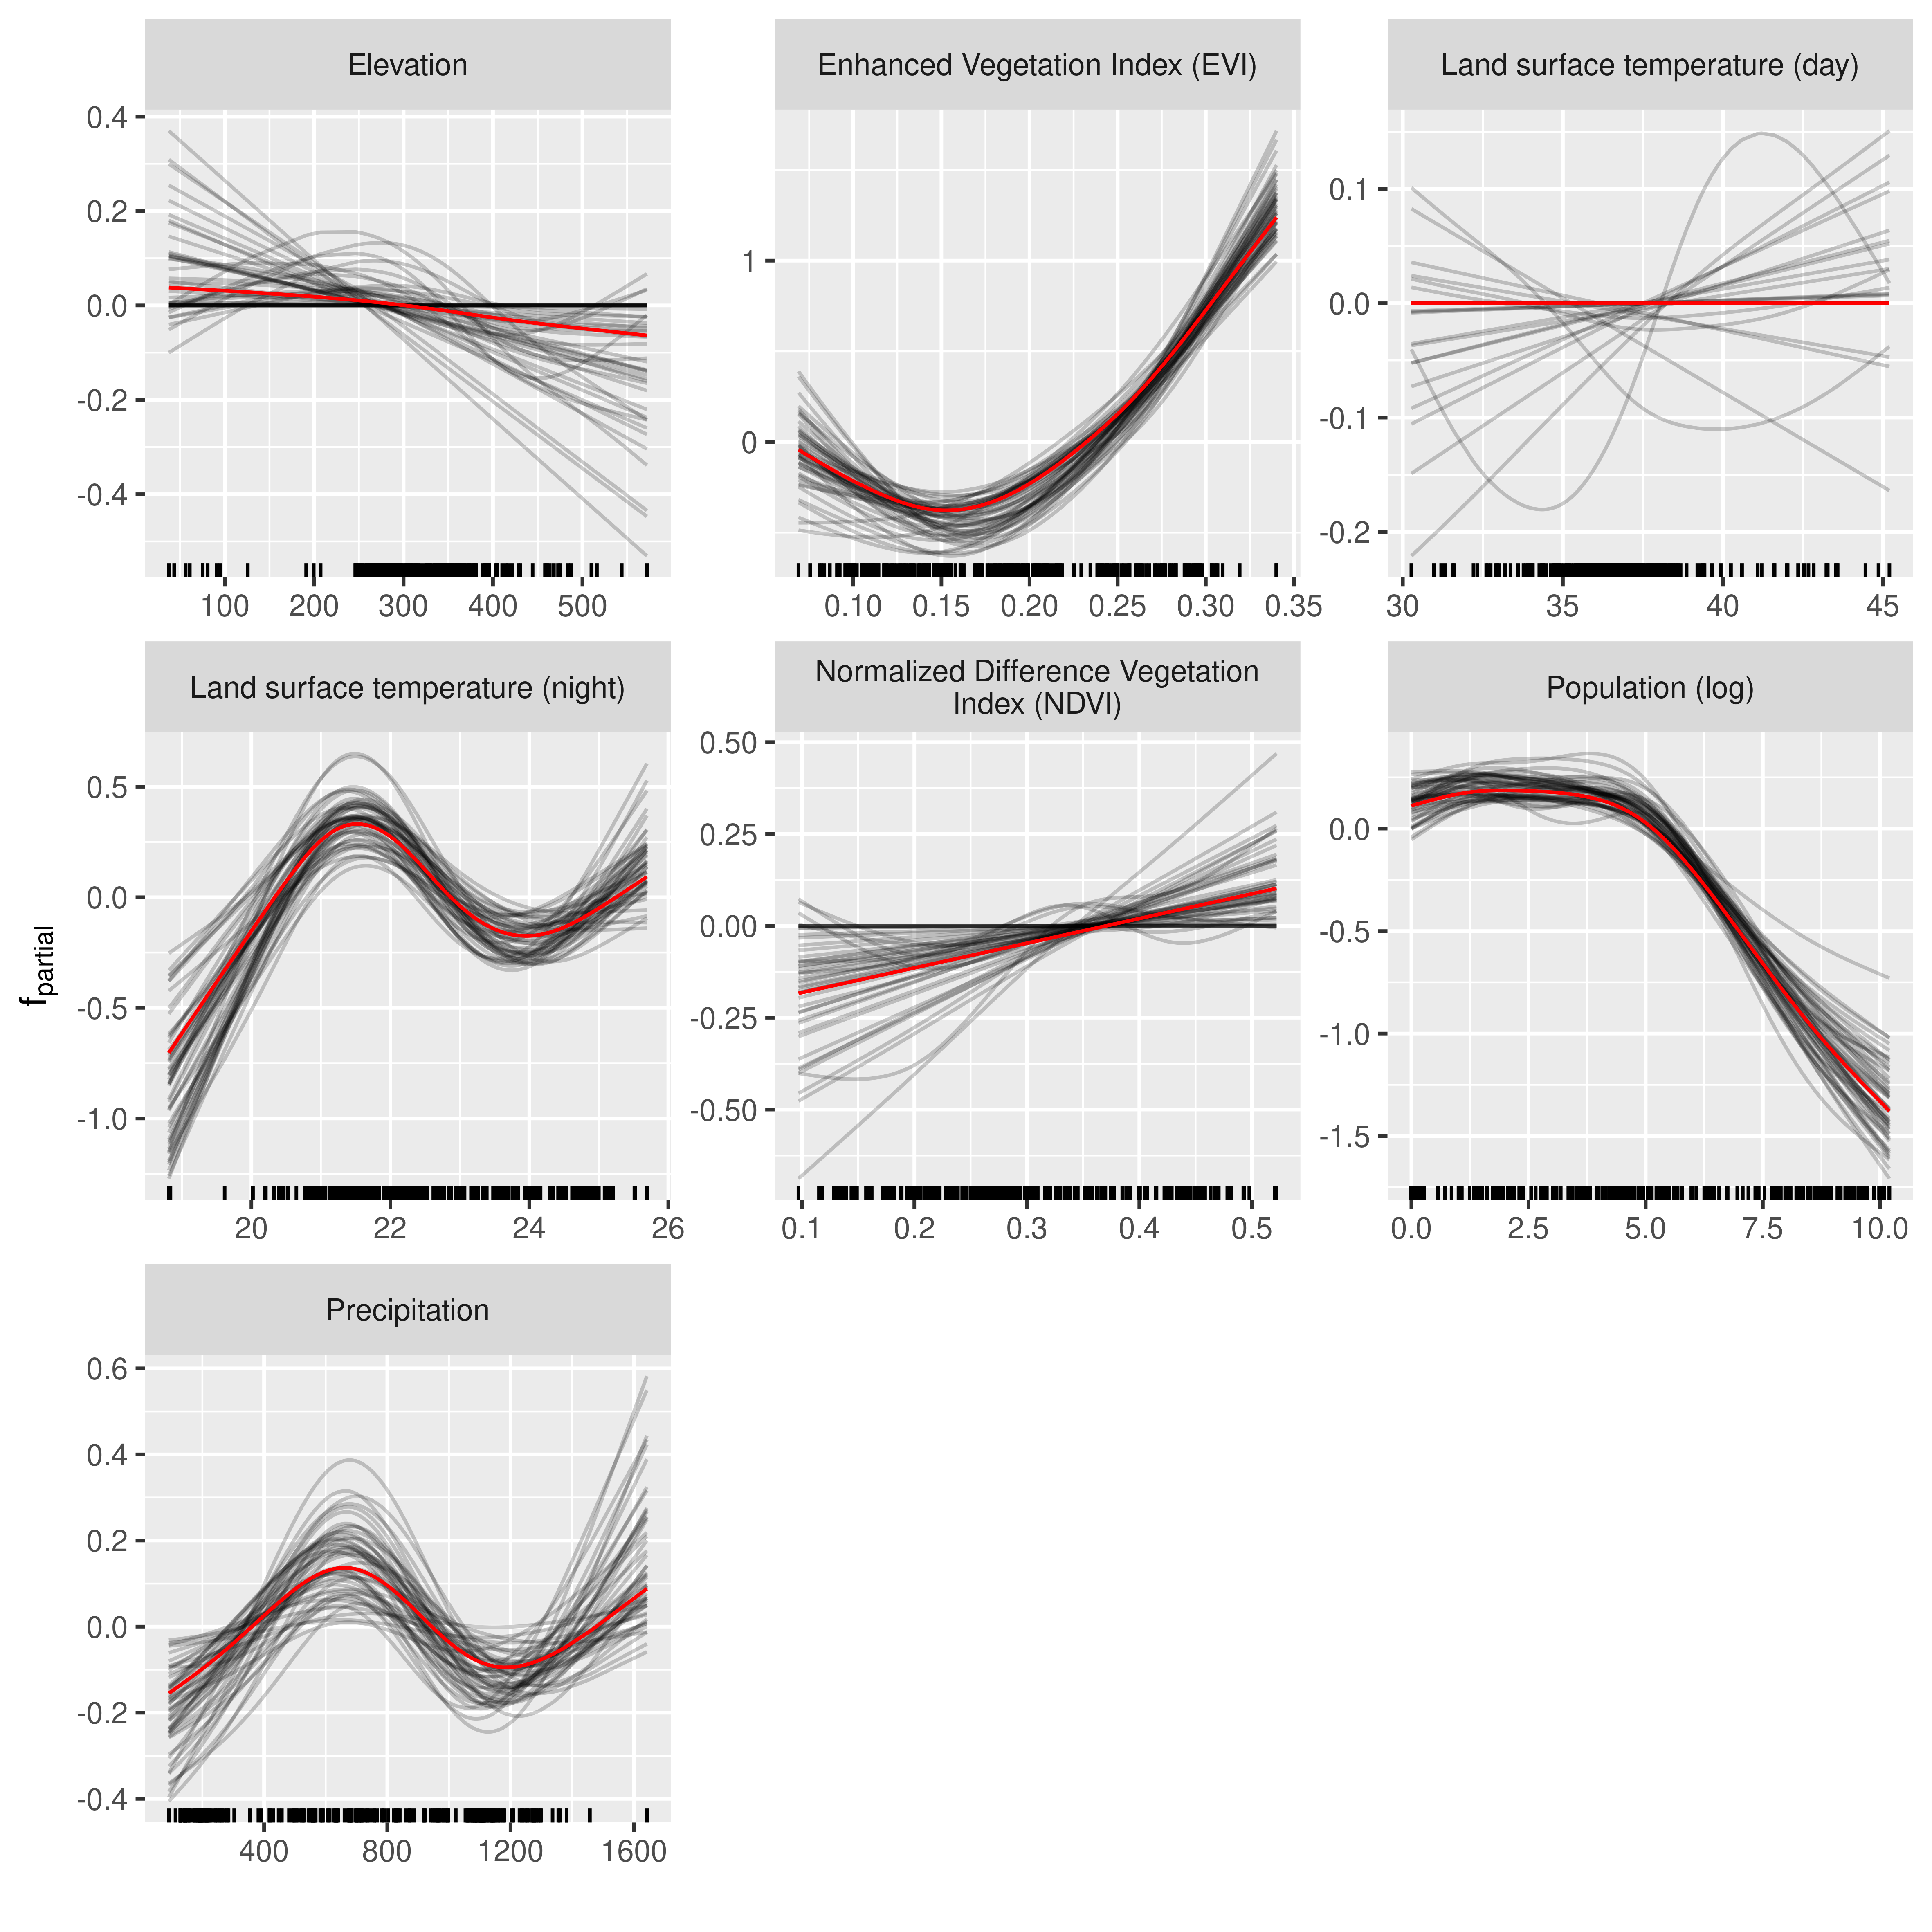
\includegraphics[width=0.9\textwidth, keepaspectratio]{figures/mali_maineffects.png}
	\caption{Geographic malaria risk in Mali: partial effects of the continuous covariates. The red line indicates the main model and the grey lines indicate the estimated effects from 50 bootstrap samples.}
	\label{fig:mli_main_effects}
\end{figure}

The partial effect of the spatial smooth is plotted in \autoref{fig:mali_spatialeffect}. For the country's west and north-eastern part a negative partial effect can be identified, in the mid-eastern part, towards the border with Burkina Faso, a positive partial effect. The standard error of the spatial effects is shown in \autoref{fig:mali_spatialeffectuncertainty}. The estimated effect is estimated stable in the southern part (where the majority of cluster locations are located) and shows a higher standard error in the northern parts. Given the lack of data north of the $18^\circ$, only the grid-cells south of the $20^\circ$ are plotted (c.f. the observed cluster locations in \autoref{fig:mli_climatezones}).

\begin{figure}[!th]
	\centering
	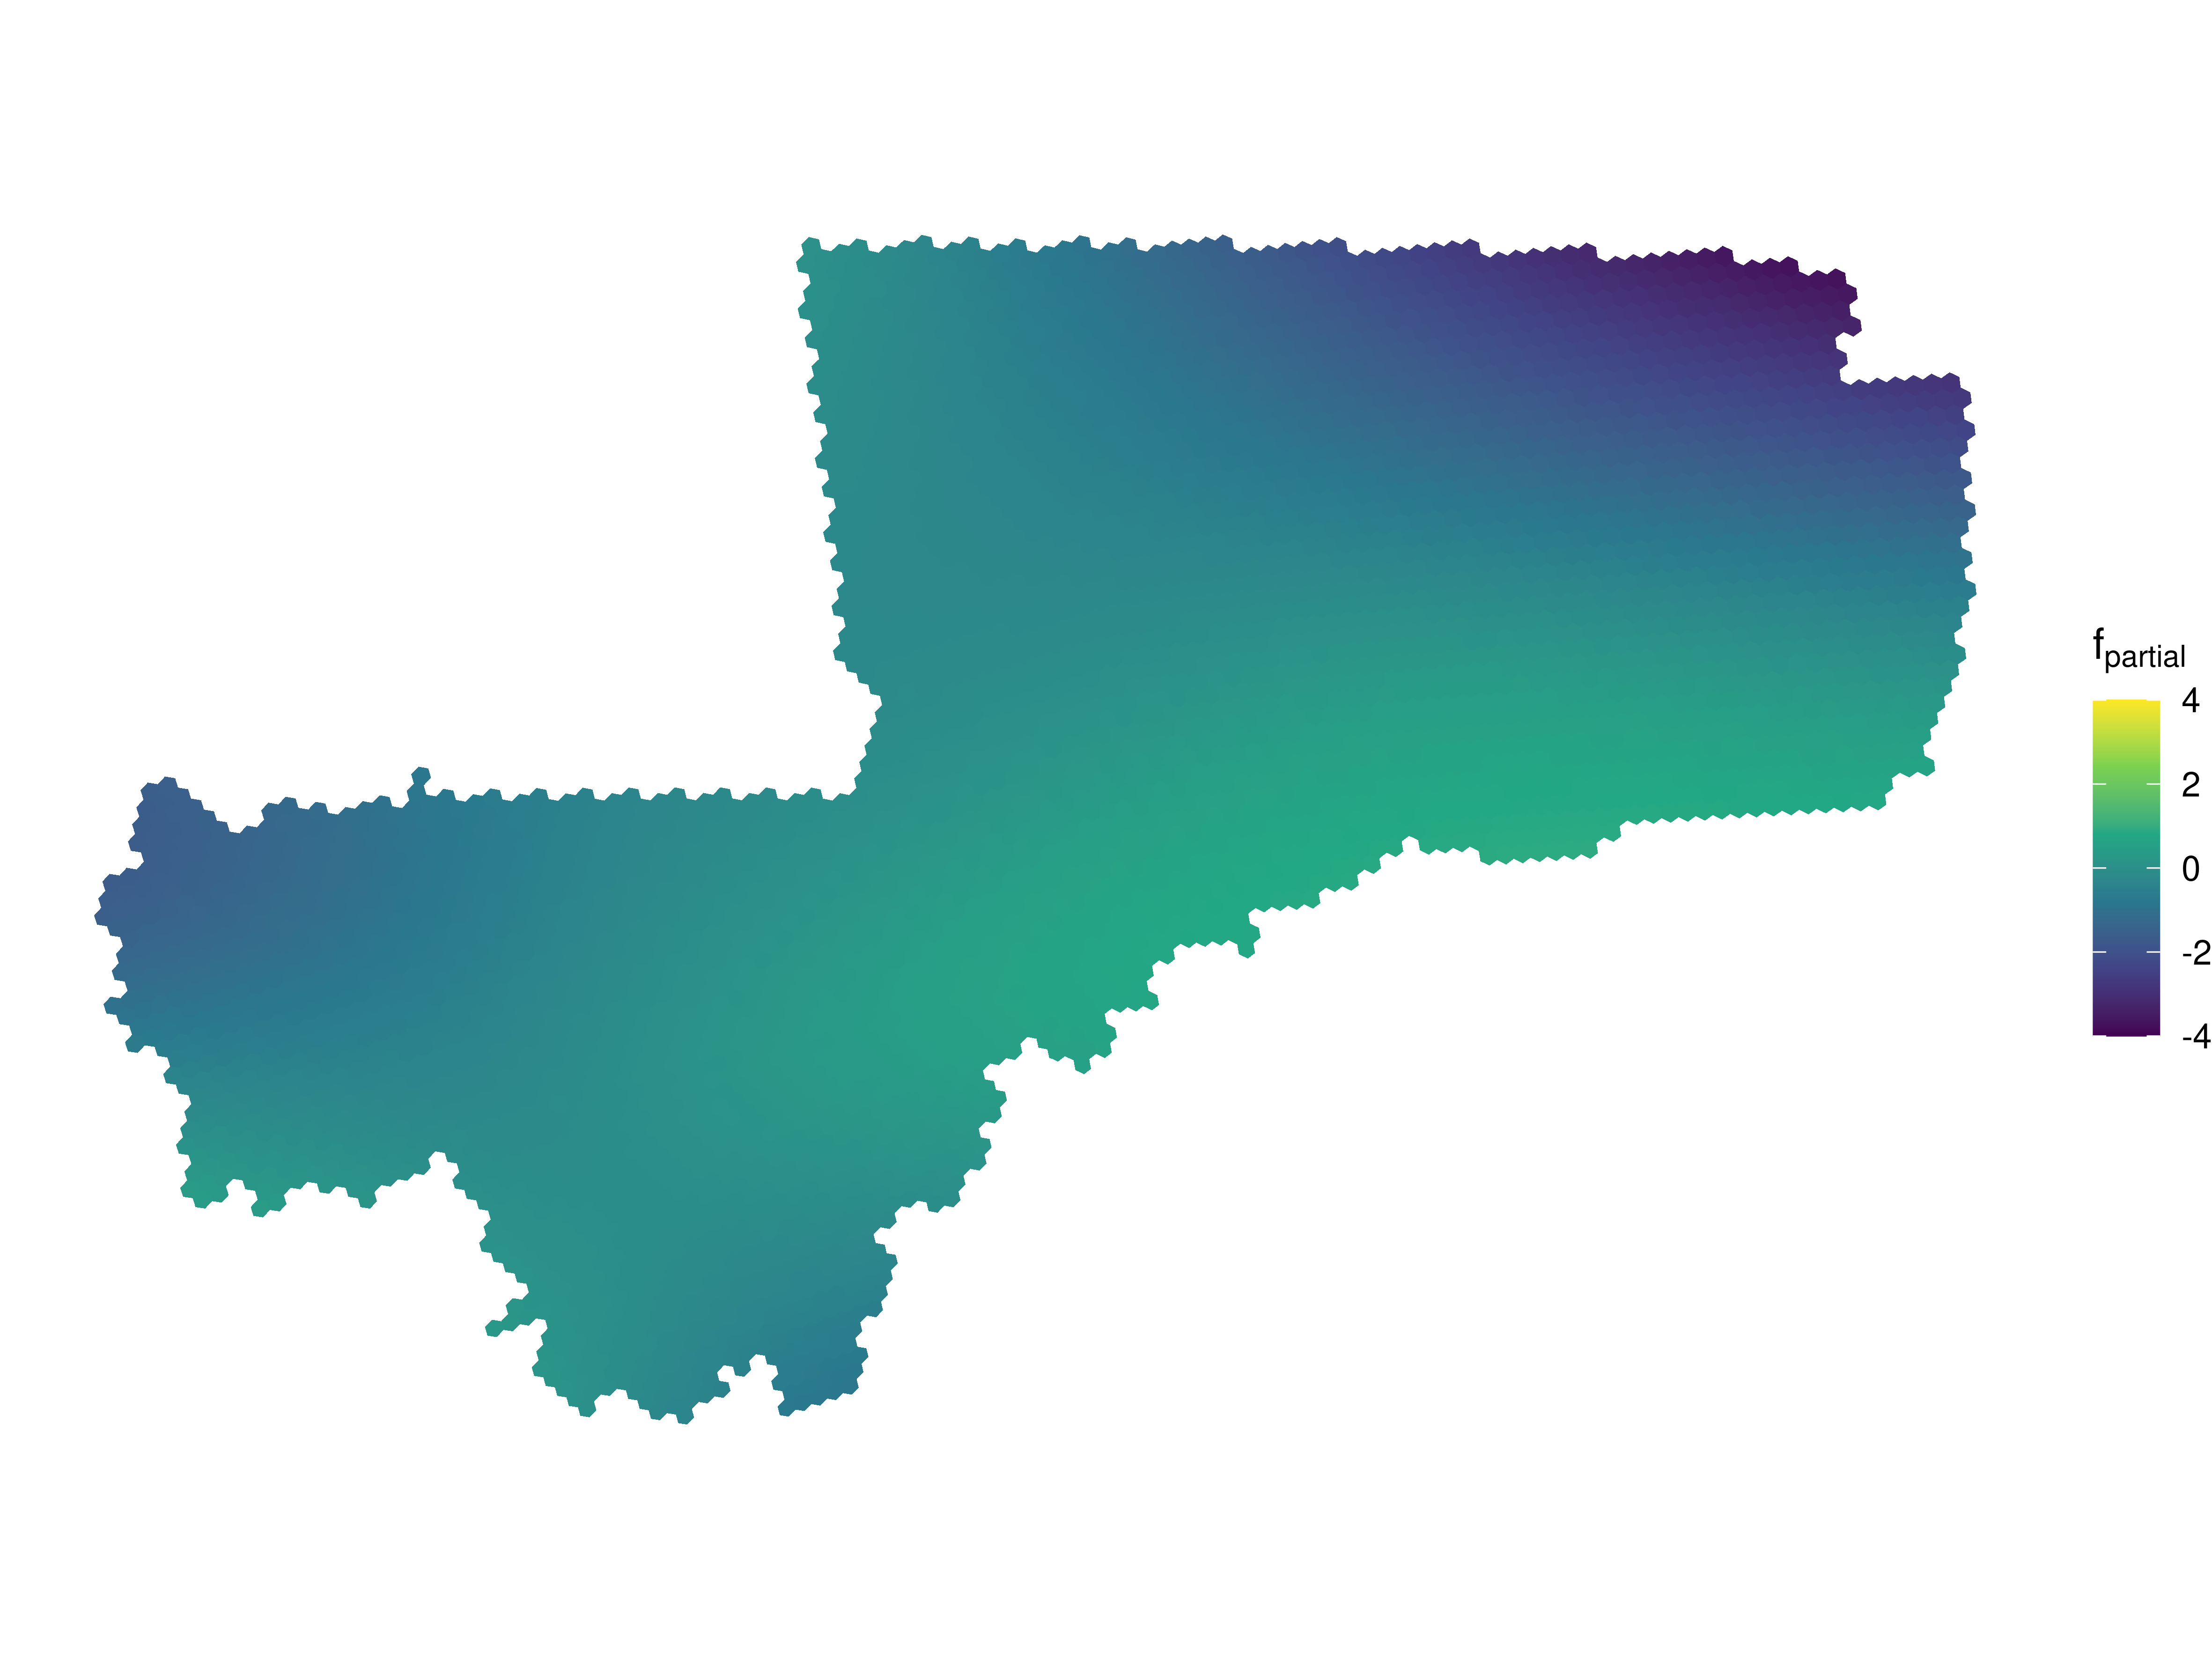
\includegraphics[width=0.9\textwidth, keepaspectratio]{figures/mali_spatialeffect.png}
	\caption{Geographic malaria risk in Mali: estimated partial effect of the bivariate P-splines.}
	\label{fig:mali_spatialeffect}
\end{figure}

\begin{figure}[!th]
	\centering
	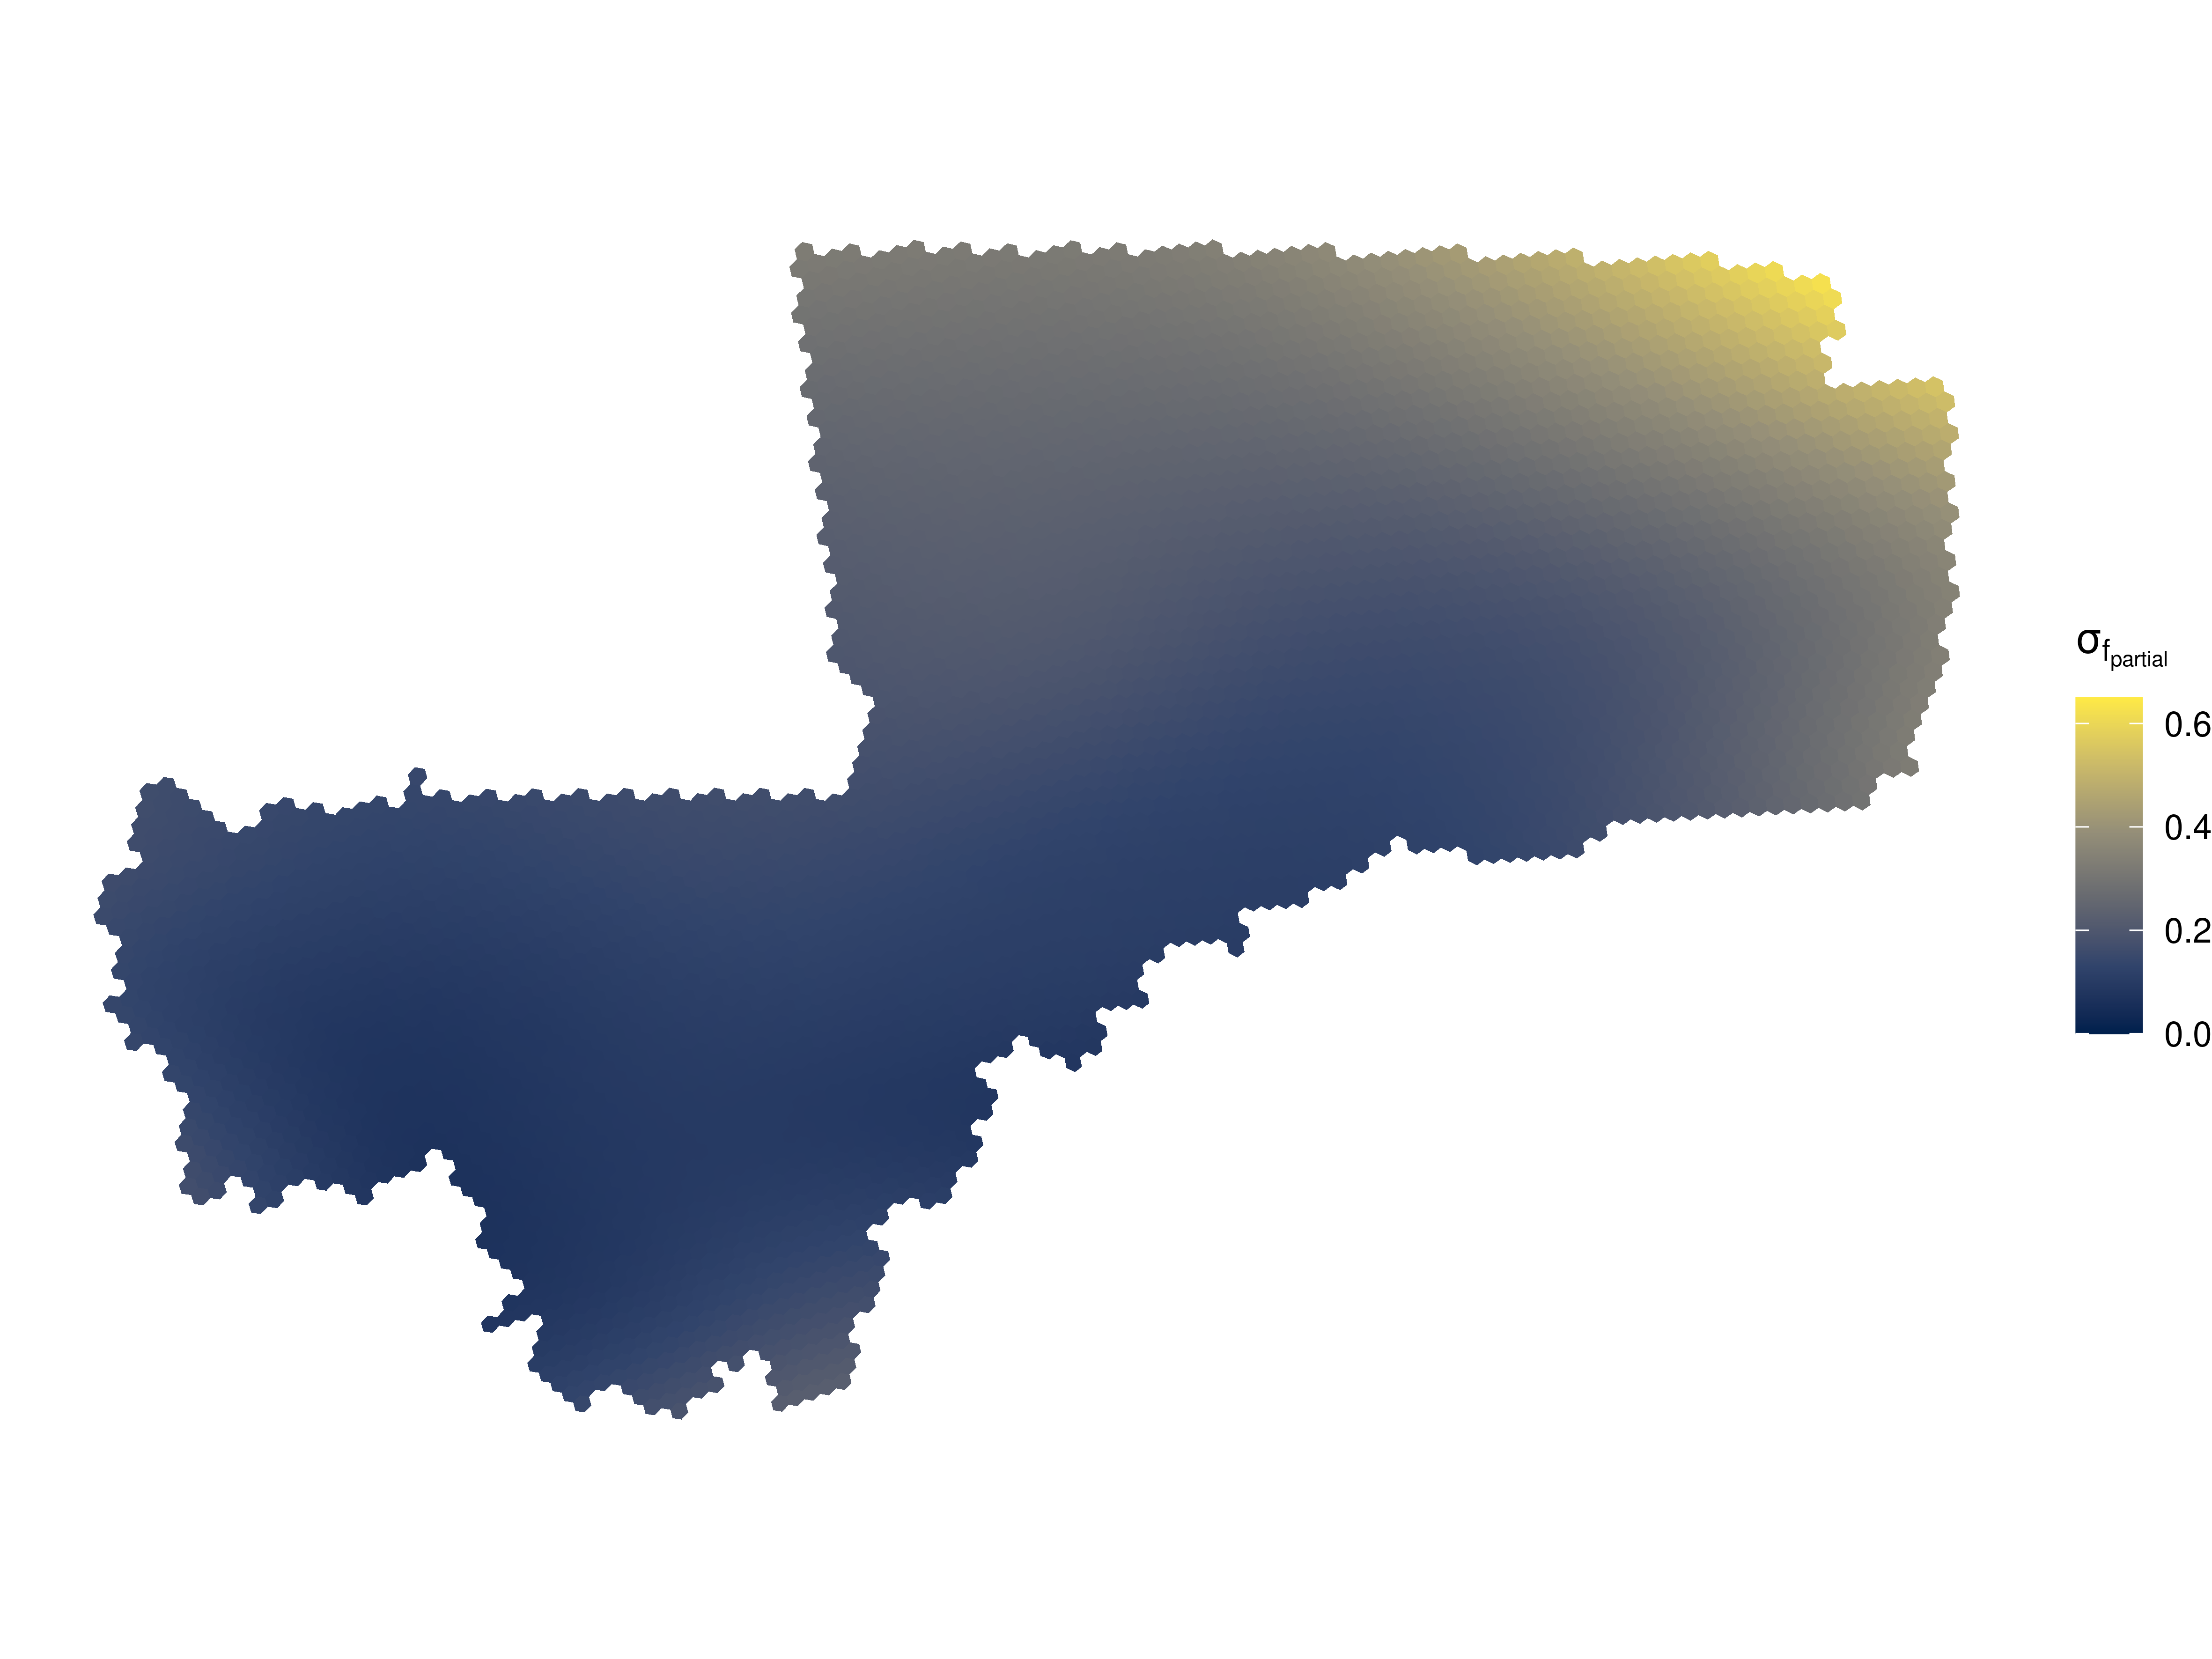
\includegraphics[width=0.9\textwidth, keepaspectratio]{figures/mali_spatialeffectuncertainty.png}
	\caption{Geographic malaria risk in Mali: standard error of the estimated partial effect based on 50 bootstrap samples.}
	\label{fig:mali_spatialeffectuncertainty}
\end{figure}

Based on the model, it is feasible to construct maps of the predicted risk of malaria throughout the country on a fine-scaled grid. \autoref{fig:mali_predictions} plots the predicted values $\hat{\mu}$. I provide additional details on the construction of the grid in the supplementary material. The north, dominated by desert or semi-desert lands is estimated at very low risk. The lower half shows higher mean prevalences, particularly on the border towards Guinea (southwest). Furthermore, distinct geographical features such as the capital Bamako in the southwest and parts of the Niger river in the east can be distinguished from the estimated near zero risk. The predicted risk for each location can be accessed in the enclosed code repository. 

Maps of predicted risk at such high resolution may mask high uncertainty in the predictions \autocite{dongModelingPresentationVaccination2021}. Therefore, I include maps of the 10\% and 90\% quantile as well as the standard error of the predictions over the bootstrap samples. The figures can be found in the supplementary material.

\begin{figure}[!t]
	\centering
	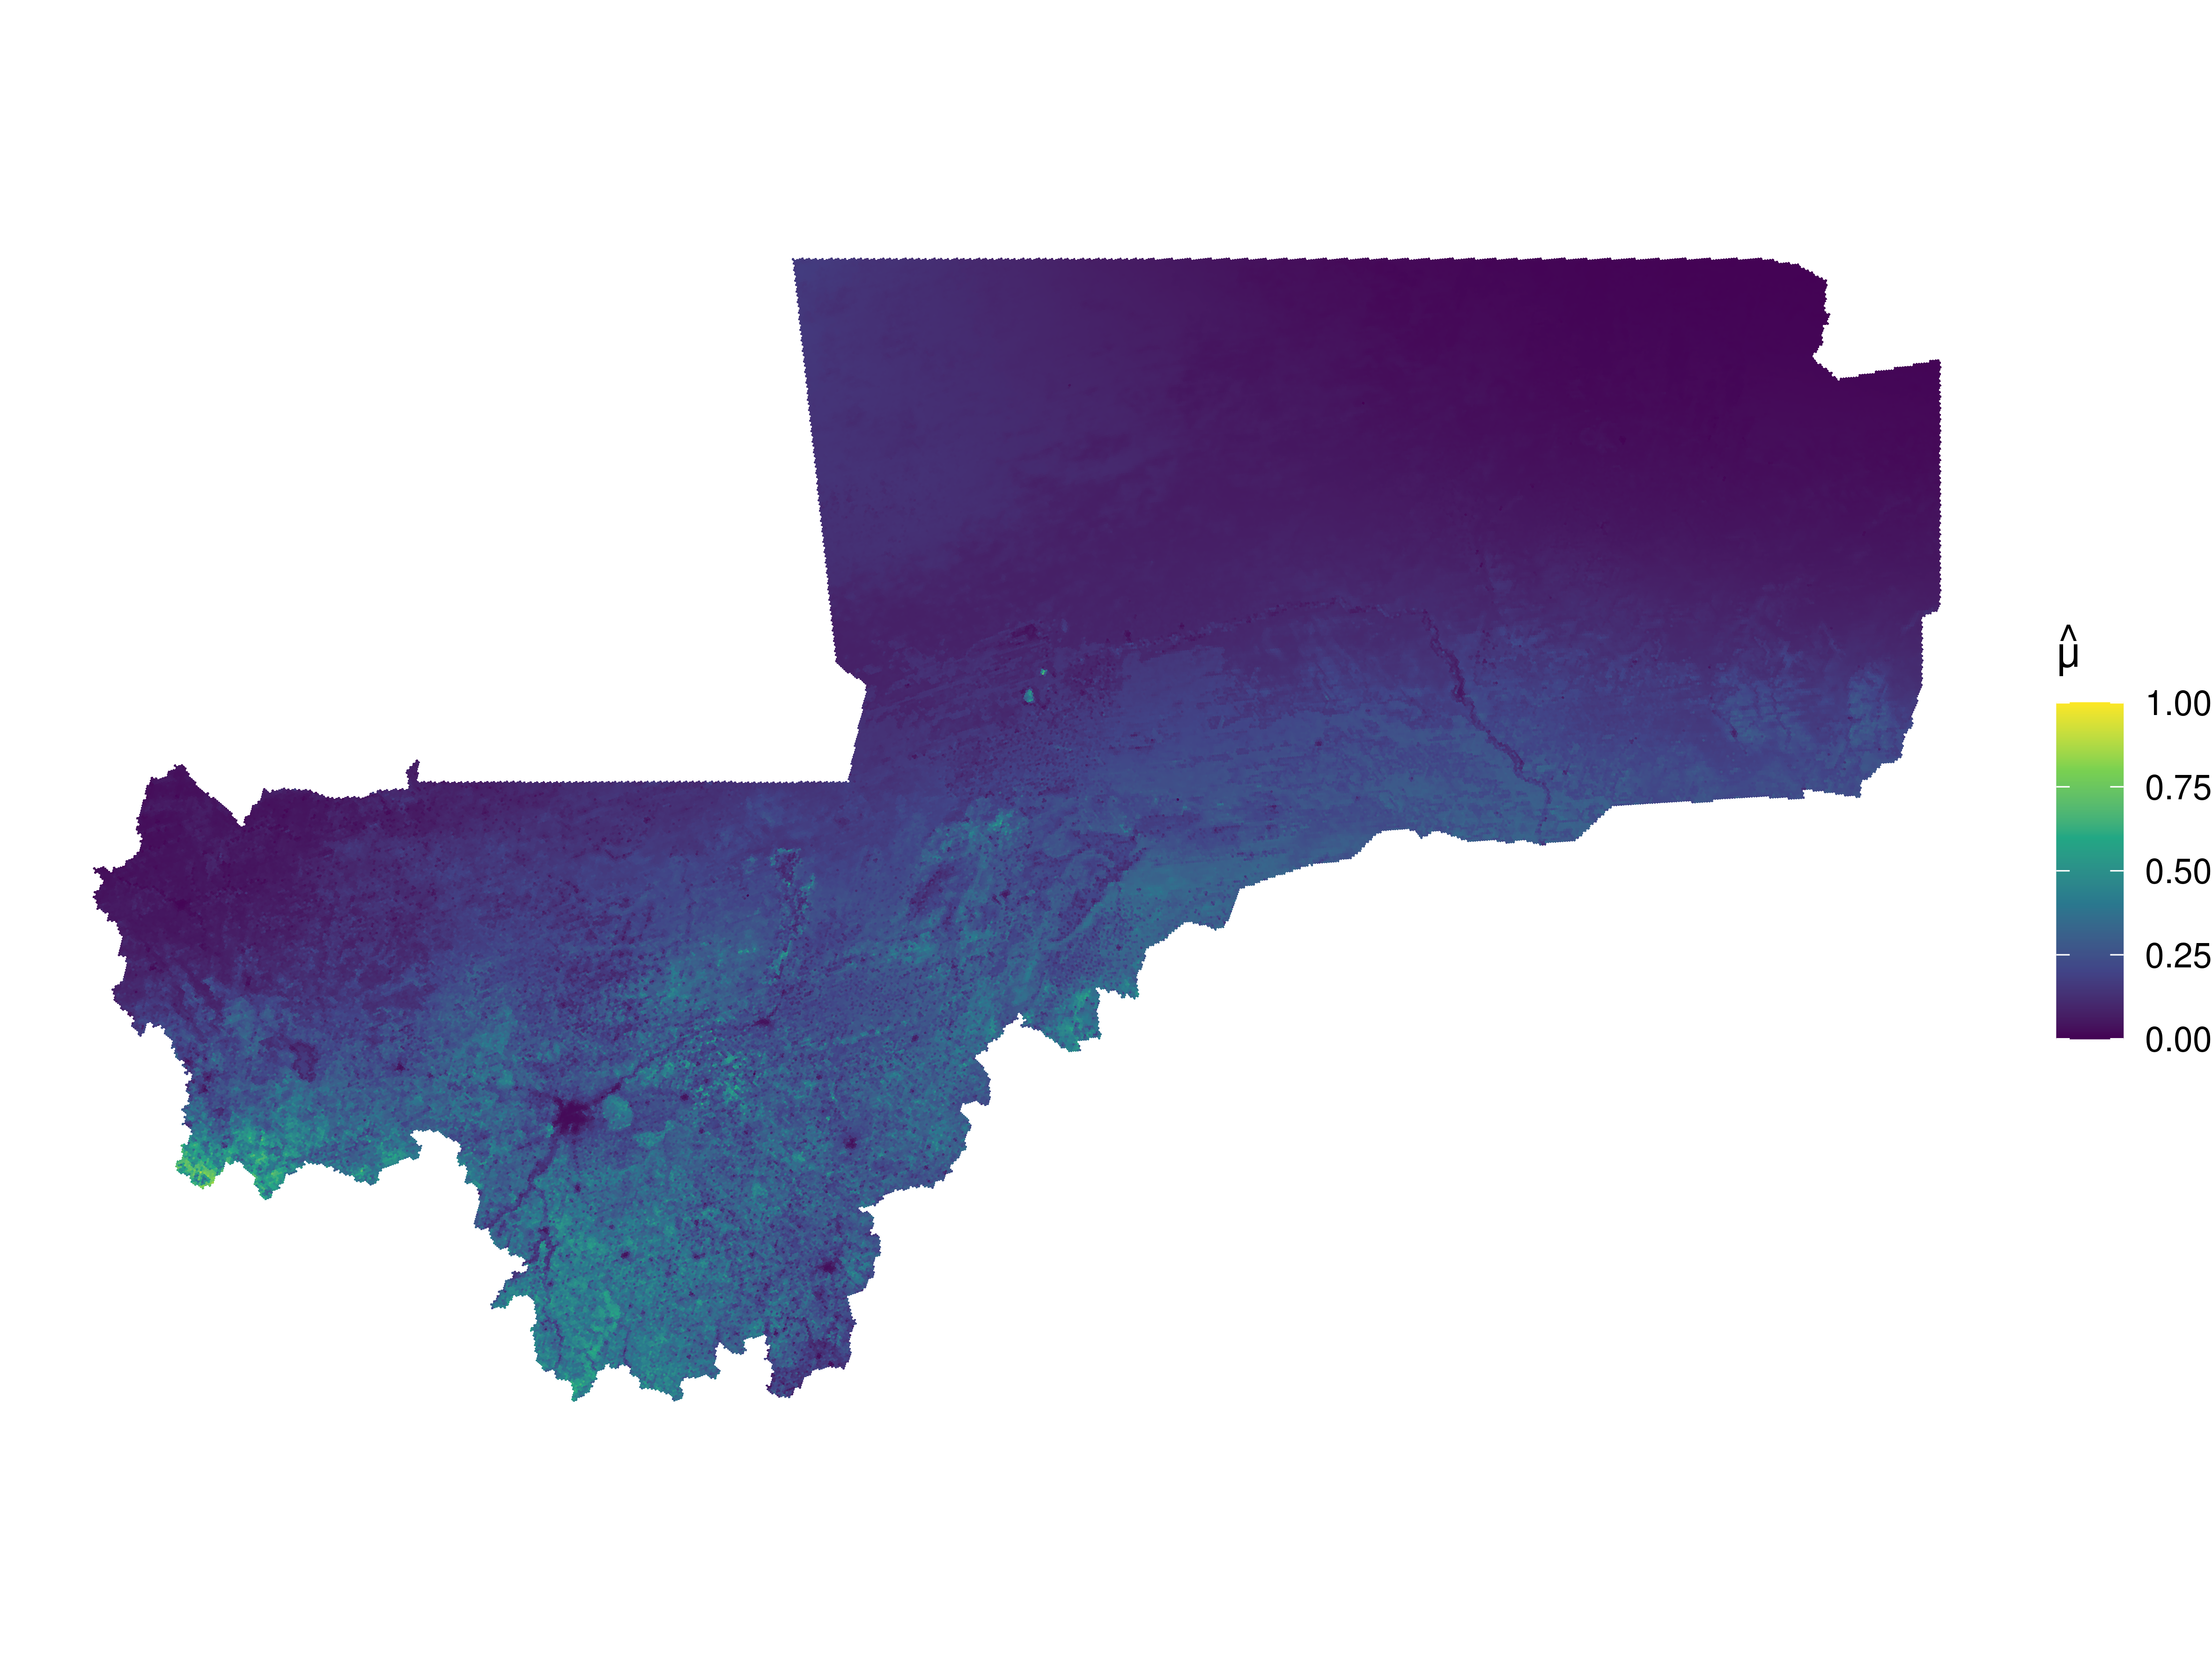
\includegraphics[width=0.9\textwidth, keepaspectratio]{figures/mali_predictions.png}
	\caption{Geographic malaria risk in Mali: predicted risk of malaria for children below the age of five. }
	\label{fig:mali_predictions}
\end{figure}


\subsubsection*{Construction of subnational prevalence estimates}

The predicted grid-level risk estimates can be aggregated to obtain an estimate for the subnational prevalence at the admin level 1 or 2. Assuming a fixed proportion of under five-year-olds to the population throughout the country, the estimate is obtained by the average risk, weighted by the population over the area of interest. To assess how well these estimates compare to the design-based estimates, \autoref{fig:mali_estimatesadmin1} shows the design-based and model-based estimates side-by-side. At the mean, the model-based estimates track closely the design-based estimates for five of the nine regions and recover the design-based estimates. The confidence intervals are the quantiles from the bootstrapped models. Certainly, the confidence intervals of the model-based approach are over-confident and likely provide poor coverage of the true prevalence.

The differences between the estimates for the regions Koulikoro, Mopti, Segoú and Sikasso, nevertheless, demand further investigation. Two possible sources of error are the urban-rural indicator (specifically, if the baseline prevalence in each is substantially different) and the gridded population maps.\footnote{Rather than the GHSL gridded population map employed in this analysis one could have used WorldPop \autocite{bondarenkoCensusProjectiondisaggregatedGridded2020}. However, a complete comparison is beyond the scope of this manuscript.} For example, for Koulikoro, the share of the urban population provided in the survey report is 5.5\% while the estimate based on the gridded population maps is 41.7\%. Though the population census is from 2009, and it is not inconceivable that a fast urbanization process leads to strong differences in urban-rural fractions, the hypothesis of underestimating the rural population is consistent with the strong underestimation of the malaria prevalence in those regions. The dependence of such approaches on gridded population maps warrants further research. Therefore, the estimates for admin 2 should be interpreted with caution and can be accessed in the enclosed code repository.

\begin{figure}[!t]
	\centering
	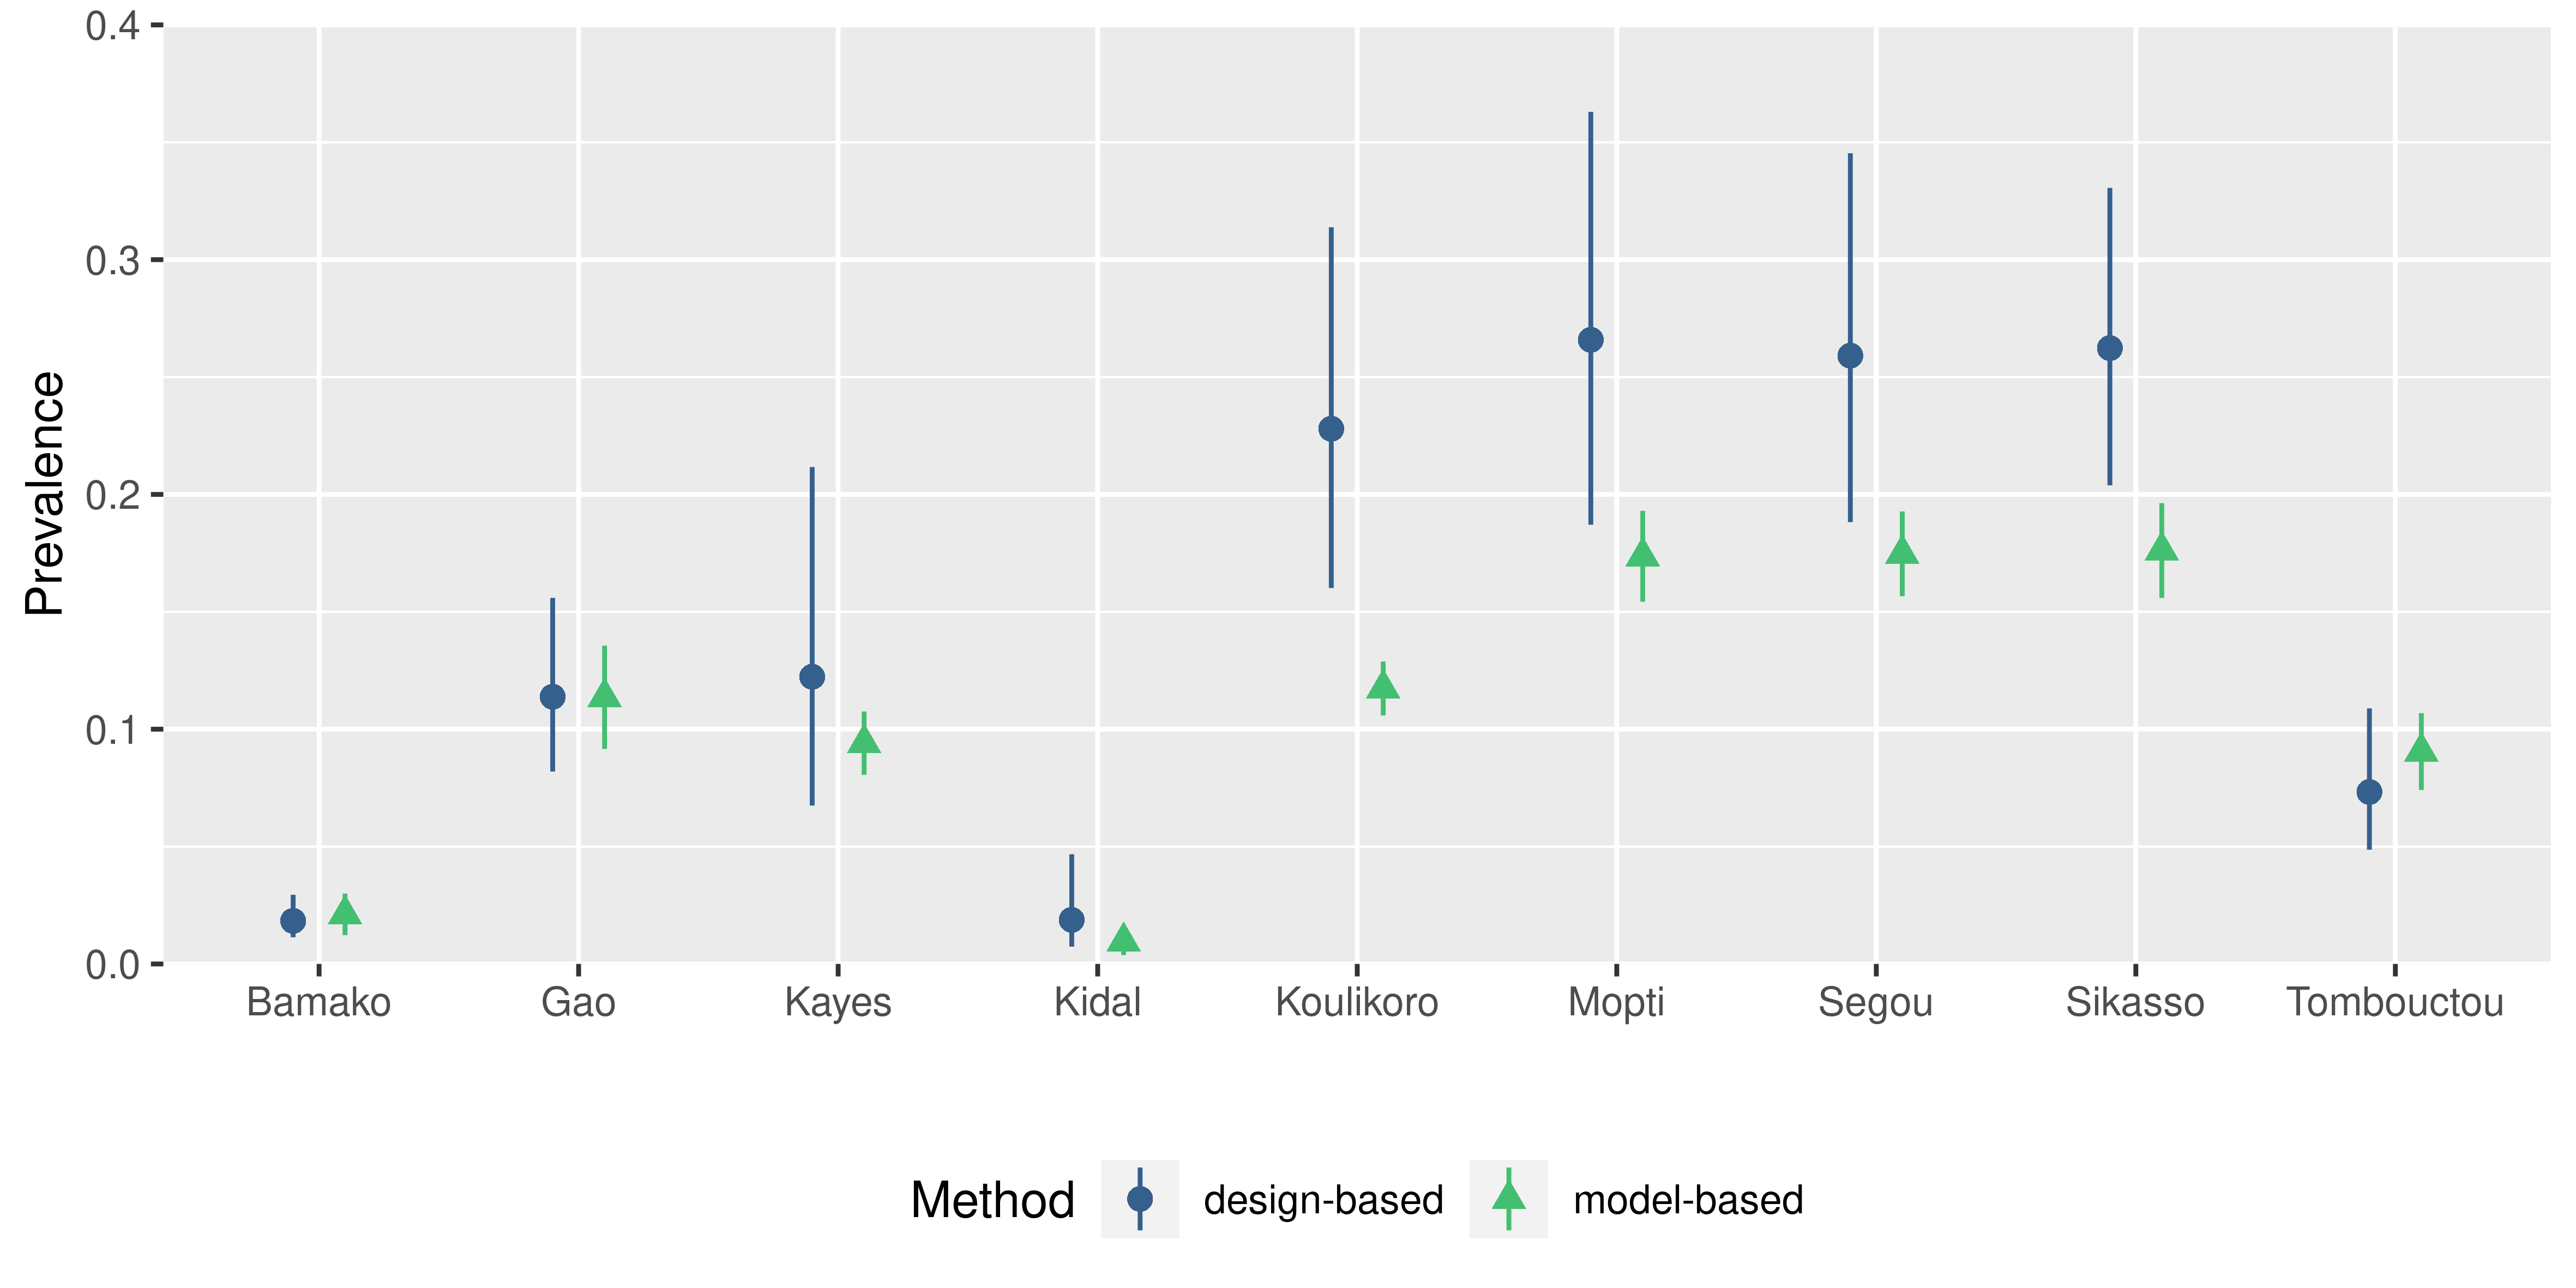
\includegraphics[width=0.9\textwidth, keepaspectratio]{figures/mali_estimatesadmin1.png}
	\caption{Geographic malaria risk in Mali: comparison of design-based estimates and model-based estimates for admin 1. Error bands are 95\% confidence intervals, for the model-based approach based on bootstrap quantiles.}
	\label{fig:mali_estimatesadmin1}
\end{figure}


\subsubsection*{Comparison to alternative approaches}

In a similar malaria mapping study, \textcite{bhattImprovedPredictionAccuracy2017} propose a stacked ensemble approach to improve prediction accuracy. Briefly, the fitted values of different state-of-the-art algorithms (gradient-boosted trees, random forests, etc.) are weighted and included in a geo-statistical model which accommodates spatial variation unaccounted for in the first level. The authors find the approach to be highly competitive in predictive tasks such as malaria prevalence estimation. The specifics can be found in \textcite{bhattImprovedPredictionAccuracy2017}. 

The approach proposed herein can account for non-linear and spatial effects in a single framework without the need for additional calibration of intermediate levels. Furthermore, the data is binomial, provided per cluster $c$ as the number of children $y_c$ that tested positive out of a total number of tested children $n_c$. The authors compute the cluster-level prevalences $\hat{p}_c = y_c / n_c$ and logit transform the estimates to obtain values with continuous support. This allows the use of common software packages for gradient-boosting trees and random forests, however, it does not respect the binomial nature of the data. In the proposed approach, the binomial distribution can be modelled directly as response distribution and allow inference about underlying risk. In addition, we obtain a semi-parametric model that can uncover important ecological correlations. 

Similarly, \textcite{weissReexaminingEnvironmentalCorrelates2015} study environmental correlates of malaria. The authors compile a set of more than 50 million (!) possible predictors by an array of transformations and combinatorial interactions. The set of possible terms was successively reduced using information criteria, to identify relevant risk predictors and the corresponding functional form. Though the authors use binomial GLMs, variable selection based on information criteria is generally considered as unstable \autocite[see, for example, the discussion in][Section 2.2]{mayrGeneralizedAdditiveModels2012}. Employing a component-wise boosting approach such as described herein avoids such pitfalls and allows for competitive predictive performance and effect selection. 


\section{Discussion}\label{sec:discussion}

In this manuscript, I demonstrated the framework of component-wise boosting to identify risk factors of two common prevalent health conditions in sub-Saharan Africa. Boosting, a method stemming originally from the machine learning literature for classification has been continuously developed in the last decade to address a variety of common statistical tasks and provide inference in moderate to high-dimensional regression settings. I have reviewed those in \autoref{sec:methodology}. In particular, boosting compares favourably with other approaches if the variable selection is desired or necessary, either because of the dimensionality induced by covariates or because the understanding of the functional form of effects is crucial.  

In the case study on chronic childhood malnutrition, the analysis underscored the necessity to consider the non-linear effects of potential risk factors, such as the child's age. Studying the environmental correlates of malaria reiterated this point, as the specification outperformed alternative definitions and even boosted trees, a method often employed as the default. In contrast to approaches presented in the literature on disease prediction, the component-wise boosting approach yields an interpretable model and allows for response distributions appropriate for the prevalence data at hand. It would be an interesting task to extend the malaria risk analysis to evaluate the predictive performance on cross-country data sets with multiple survey rounds and an extended set of explanatory variables with comparison to the distributional random forests approach \autocite{schlosserDistributionalRegressionForests2019}. 

Recent research has studied the merits of including 'alternative' data sources in the estimation of poverty or other local development indicators.\footnote{See, for example, \textcite{jeanCombiningSatelliteImagery2016, papeEstimationPovertySomalia2019, aikenMachineLearningPhone2022, ziuluPovertyMappingInnovative2022, aikenProgramTargetingMachine2023}.} For instance, \textcite{steeleMappingPovertyUsing2017} explored embedding mobile operator call detail records (CDRs) for the small area estimation of poverty. Those data are usually provided in a collection of statistics that can be derived from call data and aggregated at the unit of interest. But it is not clear which statistics are informative for the task. In such situations, one obtains tasks that boosting tends to handle very well. While the default approach in predictive modelling usually encompasses nonparametric decision trees, simpler additive models may perform competitively. This has also been shown elsewhere \autocite{kapoorLeakageReproducibilityCrisis2022}. Besides, interpretable models are often desired if policy decisions are based on them \autocite{rahmanPredictiveAnalyticsChildren2021}.

Even so, by employing boosting, one trades off conventional statistical concepts such as the quantification of uncertainty in the estimates by improved generalisation performance and intrinsic effect selection. If this trade-off is useful, will depend on a case-by-case basis. In these case studies, I used subsampling and bootstrap replications to assess variability in the estimates. While these approaches are straightforward to implement, they are computationally very intensive and do not necessarily guarantee coverage of the intervals derived, making statistical inference difficult. If a proper uncertainty quantification of model parameters is required, Bayesian hierarchical models such as those commonly employed in the geo-statistical framework are likely advantageous. Here, a clear conceptualisation of the objective of each research design is imperative, also to maintain trust in decisions derived from complex statistical approaches \textcite{broderickTaxonomyTrustProbabilistic2021}.

The literature on monitoring population health statistics has developed incredibly fast in recent years, providing models for the most followed statistics. But there still seems to be a wider gap in the treatment of data-sparse and conflict settings. The absence of official data has motivated much work in the inclusion of remotely sensed data. Obviously, there is a clear limit on what can be inferred from such data to understand population health statistics. Since the association between predictors and outcomes is likely noisy, much more promising is the merge of multiple data sources, such as household-, high-frequency phone surveys, and local assessments. There, careful modelling of the bias is important to draw correct inferences,\footnote{For a combination of survey data and 'novel data' see, for instance, \textcite{alexanderCombiningSocialMedia2022, hsiaoModelingBiasDigital2023}.} and provides many important avenues for research.

There is a broader case to be made for predictive modelling for development and epidemiological applications \autocite[e.g.,][]{greenoughMappingCaseGeospatial2019}. The component-wise boosting approach discussed herein can make some important contributions in this direction by, for example, employing appropriate response distributions, improving interpretability through model-building, and estimating non-linear and spatial effects of interest, particularly where generalisation performance is crucial. The appropriateness of statistical learning methods, however, will depend on the inferential objective of the research design.



\section*{Acknowledgements}

I would like to express my gratitude to my supervisor, Cornelius Fritz, who guided me throughout this project. I would also like to thank Yanchun Zhang for enabling my internship at the Human Development Report Office, United Nations Development Programme, in the spring of 2022. It was there where I first learned about the literature on the statistics behind monitoring socio-economic development that has inspired much of the work done in this manuscript. Camila and Paul, I would like to thank you for many thoughtful discussions on political science, statistics, and the philosophy of science, I appreciated them very much at this university. Finally, Yaiza, for keeping me sane throughout this period, thank you very much. 


\newpage
\printbibliography[title=References, heading=bibintoc]

\cleardoublepage
\begin{refsection}
\appendix
\addtocontents{toc}{\protect\setcounter{tocdepth}{1}}


\section{Supplementary Material}\label{sec:supplementary-material}

\subsection{Data sources, availability and additional details}\label{sec:data-sources-availability-and-additional-details}

Survey regions and country borders were retrieved from the Spatial Data Repository \autocite{icfinternationalSpatialDataRepository2022} and the Database of Global Administrative Boundaries (GADM) \autocite{globaladministrativeareasGADMDatabaseGlobal2022}. The remotely sensed covariates in \autoref{sec:geographic-malaria-risk-in-mali} are mean values over the year preceding the start date of the survey fieldwork. All raster files are open-access and were retrieved from the Google Earth Engine API \autocite{gorelickGoogleEarthEngine2017} or the respective provider as described in the respective publications at a spatial resolution of 1km x 1km. 

To create a fine-scaled country grid I use the spatial unit indexing system \textit{H3: A Hexagonal Hierarchical Geospatial Indexing System} \autocite{ubertechnologiesH3HexagonalHierarchical2022}. The grid level estimates are produced for a grid of resolution 7, hexagons with an area of approximately 5km$^2$. I extract for each cluster location or hexagon centroid the value interpolated from the values of the four nearest raster cells. One exception is the population data, where exact areal extraction is used to obtain a consistent disaggregation of population totals. 


\subsection{Computational implementation}\label{sec:computational-implementation}

All analyses were conducted in {\tt R} 4.2.2 \autocite{rcoreteamLanguageEnvironmentStatistical2022} and Python 3.9.13. The code files and data requirements to fully replicate this work along with additional results are included in the corresponding GitHub repository.\footnote{See \url{https://github.com/danielseussler/ssahealthriskfactors}.}

The described models were fitted using the {\tt mboost} and {\tt gamboostLSS} packages \autocite{hothornMboostModelBasedBoosting2022, hofnerGamboostLSSPackageModel2016}, see also \textcite{hothornModelbasedBoosting2010} for an introduction. The following {\tt R} packages provided helpful functions for evaluation metrics, raster extraction and survey data analysis: \textcite{hamnerMetricsEvaluationMetrics2018, pfefferMalariaAtlasInterfaceGlobal2018, watsonRdhsPackageInteract2019, lumleySurveyAnalysisComplex2020, hijmansGeodataDownloadGeographic2022, bastonExactextractrFastExtraction2022}. 


\subsection{Distributions}
\label{appendix_distributions}

\subsubsection*{Binomial distribution}

\begin{equation*}
	Y \sim \: \Binomial(n, \mu)
\end{equation*}

For $y = 0, 1, \dots, n$ and $0 < \mu < 1$, the probability density function of the binomial distribution is 
\begin{equation}
	f(y \vert n, \mu) = \frac{n!}{y! (n-y)!} \mu ^y (1 - \mu)^{n-\mu}
\end{equation}
where the first and second moments are
\begin{align*}
	E(Y) &= n\mu, \\
	Var(Y) &= n \mu (1-\mu).
\end{align*}


\subsubsection*{Beta-binomial distribution}

\begin{equation*}
	Y \sim \: BB(n, \mu, \sigma)
\end{equation*}

For $y = 0, 1, \dots, n$, $0 < \mu < 1$, and $\sigma > 0$, the probability density function of the beta-binomial distribution is 
\begin{equation}
	f(y \vert n, \mu, \sigma) = \frac{\Gamma(n + 1)}{\Gamma(y + 1) \Gamma(n - y + 1)}
	\frac{
		\Gamma(\frac{1}{\sigma}) \Gamma(y + \frac{\mu}{\sigma}) \Gamma(n + \frac{(1-\mu)}{\sigma} - y)
	}{
		\Gamma(n + \frac{1}{\sigma}) \Gamma(\frac{\mu}{\sigma}) \Gamma(\frac{1-\mu}{\sigma})
	}.
\end{equation}
The corresponding first and second moments are 
\begin{align*}
	E(Y) &= n \mu, \\
	Var (Y) &= n \mu ( 1- \mu ) [ 1 + \sigma (n - 1) / (1 + \sigma) ].
\end{align*}
See also \textcite{rigbyDistributionsModelingLocation2019} for further information.



\subsection{Additional Results}\label{sec:additional-results}

In this section, I present additional figures and tables for the two case studies.

% latex table generated in R 4.2.2 by xtable 1.8-4 package
% Thu Jan 12 14:45:15 2023
\begin{table}[!p]
	\centering
	
	\begin{tabularx}{0.8\textwidth}{Xl}
		
		Base-learner & Frequency \\ \arrayrulecolor{black!30}\midrule
		cage & 1.00 \\ 
		csex & 1.00 \\ 
		ctwin & 1.00 \\ 
		cbord & 1.00 \\ 
		mbmi & 1.00 \\ 
		mage & 0.74 \\ 
		medu & 1.00 \\ 
		memployed & 0.22 \\ 
		mreligion & 0.98 \\ 
		nodead & 0.86 \\ 
		hmembers & 1.00 \\ 
		watersource & 0.90 \\ 
		sanitation & 0.44 \\ 
		wealth & 1.00 \\ 
		electricity & 0.30 \\ 
		radio & 1.00 \\ 
		television & 1.00 \\ 
		bicycle & 0.28 \\ 
		motorcycle & 0.82 \\ 
		car & 0.70 \\ 
		urban & 0.52 \\ 
		healthaccess & 0.36 \\ 
		cityaccess & 1.00 \\ 
		fews & 0.86 \\ 
		f(cage) & 1.00 \\ 
		f(mage) & 0.90 \\ 
		f(mbmi) & 0.40 \\ 
		f(medu) & 1.00 \\ 
		f(hmembers) & 0.48 \\ 
		f(healthaccess) & 0.68 \\ 
		f(cityaccess) & 0.98 \\ 
		f(dhsregion) & 1.00 \\ 
	\end{tabularx}

	\caption{Childhood malnutrition in Madagascar: selection frequencies of base learners over the 50 replications. The name indicates the linear effect only, f($\cdot$) is the non-linear deviation from the linear effect.}
	\label{tab:madagascar_selectionfreq}

\end{table}


\begin{figure}[!p ]
	\centering
	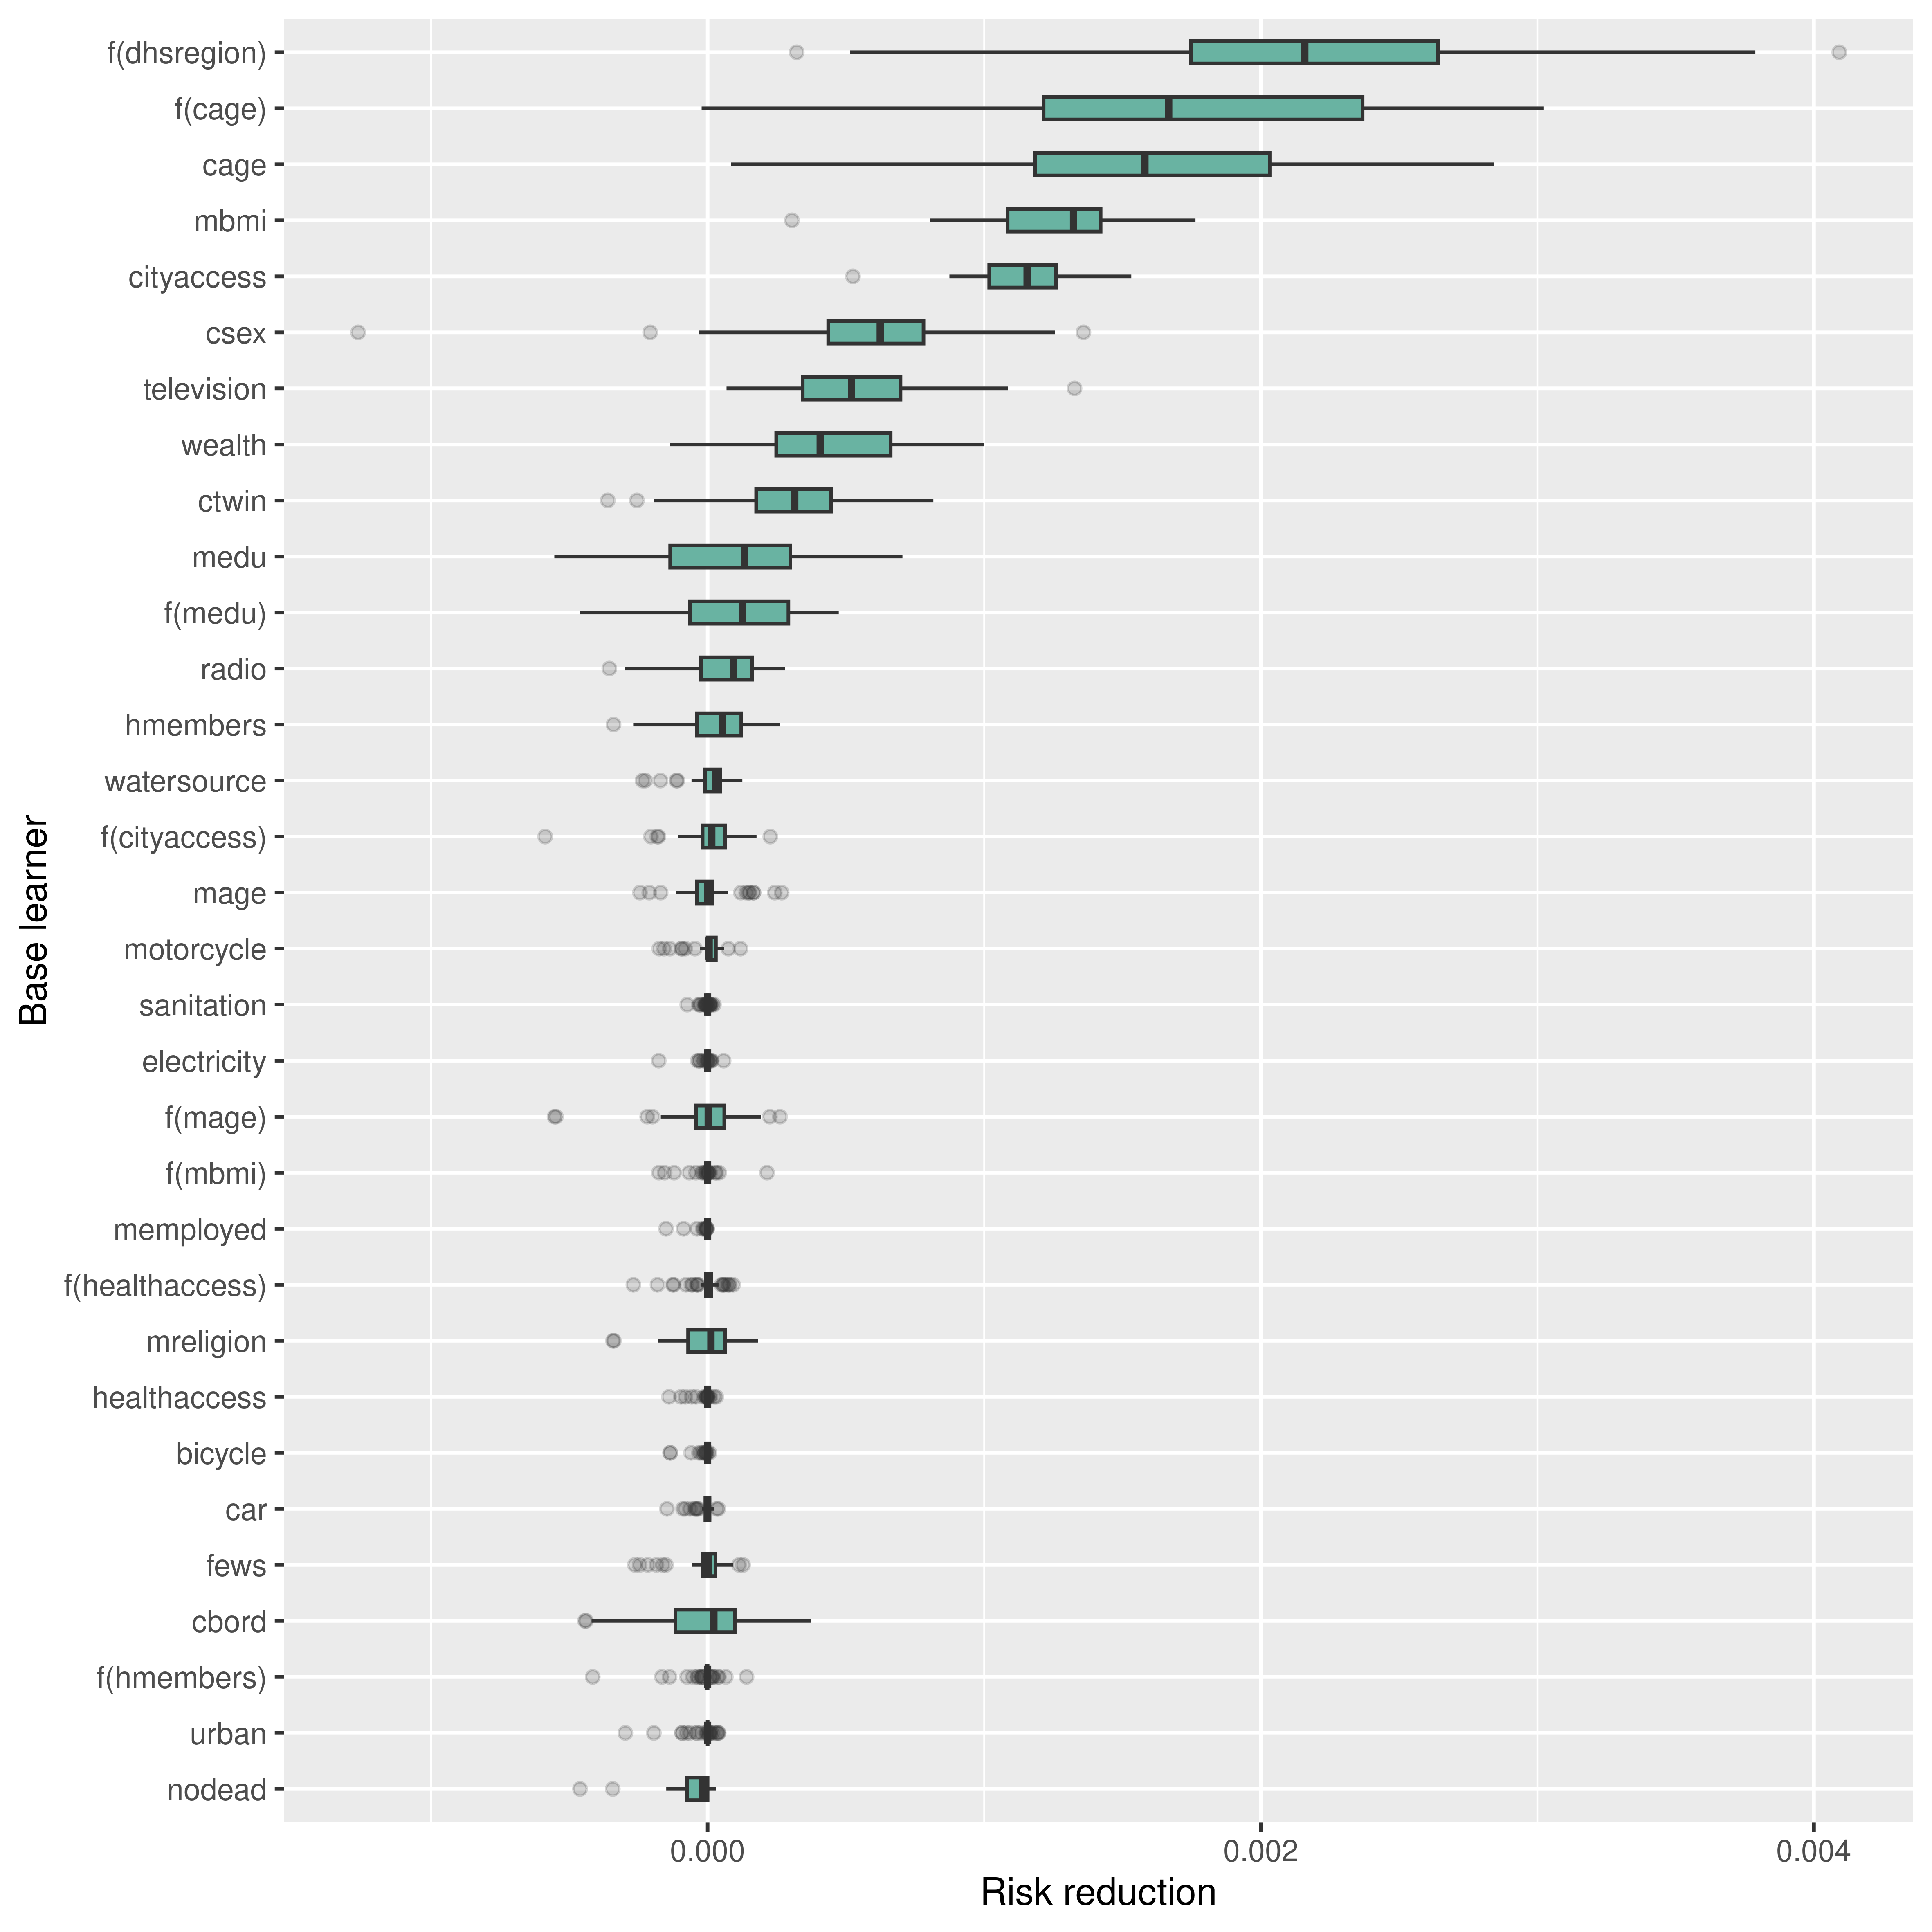
\includegraphics[width=0.9\textwidth, keepaspectratio]{figures/madagascar_variableimportance.png}
	\caption{Childhood malnutrition in Madagascar: empirical distributions of the variable importance of each base-learner by attributed risk reduction over 50 replications. Note, (small) negative risk reduction can be obtained as a fitting artefact if boosting iterations are extended beyond the maximum likelihood estimates.}
	\label{fig:madagascar_variableimportance}
\end{figure}

\begin{figure}[!p]
	\centering
	\includegraphics[width=0.9\textwidth, keepaspectratio]{figures/mali_predictionuncertainty.png}
	\caption{Geographic malaria risk in Mali: lower, upper quantiles and standard error of the predicted risk $\hat{\mu}$ based on 50 bootstrap samples.}
	\label{fig:mali_predictionuncertainty}
\end{figure}

\printbibliography[title=References]
\end{refsection}

\cleardoublepage
\section*{Declaration of Authorship}

\vspace{1cm}

I hereby certify that I have written the present thesis entitled \textit{Identification of Health Risk Factors in Developing Countries using Intrinsic Model Selection Approaches} independently and that the work contained herein is my own. All formulations and concepts taken verbatim or in substance from printed or unprinted material or the Internet have been cited according to the rules of good scientific practice and indicated by exact references to the original source. The same applies to all illustrations. The present thesis has not been submitted to another university for the award of an academic degree in this form. I understand that the provision of incorrect information may have legal consequences.

\vspace{2.5cm}
\begin{flushright}
    \hspace{10cm} Date, \ Signature 
\end{flushright}


\end{document}